% ------------------------------------------------------------------------------
% Este fichero es parte de la plantilla LaTeX para la realización de Trabajos
% Final de Grado 
% Adecuado para proyectos de desarrollo de software del Grado en Ing. Informática
% Copyright (C) Universidad de Cádiz
%% Imágenes obtenidas de Freepik (https://www.freepik.es/)
% ------------------------------------------------------------------------------


\documentclass[12pt, twoside, openright]{report}

% Paquetes LaTeX y estilos globales
\input{config/packages}
% Evita que LaTeX estire el espacio vertical para llenar páginas
\raggedbottom

% Formato del título de capítulos y secciones
% \titleformat{\chapter}[block]{\titlerule[0.8pt]\normalfont\huge\bfseries}{\thechapter.}{.5em}{\Huge}[{\titlerule[0.8pt]}]
% \titlespacing*{\chapter}{0pt}{-19pt}{25pt}
% \titleformat{\section}[block]{\normalfont\Large\bfseries}{\thesection.}{.5em}{\Large}

\titleformat{\chapter}[block]{\normalfont\huge\bfseries}{\thechapter.}{.5em}{\Huge}[{\titlerule[0.8pt]}]
\titlespacing*{\chapter}{0pt}{-19pt}{25pt}
\titleformat{\section}[block]{\normalfont\Large\bfseries}{\thesection.}{.5em}{\Large}

% Formato del código fuente con lstlisting
\lstset{
  basicstyle=\ttfamily,
  breaklines=true,
}

% Márgenes
\geometry{
    a4paper,
    margin=2.75cm
}

% Limite de profundidad del índice
\setcounter{tocdepth}{2}

% Indentación de párrafos
\setlength{\parindent}{1cm}

\renewcommand{\lstlistingname}{Extracto de código}
\renewcommand*{\lstlistlistingname}{Índice de extractos de código}

%------------ Caption debajo de las tablas
\DeclareCaptionLabelSeparator*{spaced}{\\[1.5ex]}
\captionsetup[table]{textfont=it,format=plain,justification=justified,
  singlelinecheck=false,labelsep=spaced,skip=0pt}

% Placeholder para figuras pendientes. Sustituir por \includegraphics cuando exista la captura.
\newcommand{\placeholderfigura}[2][0.55\textwidth]{%
    \fcolorbox{black!40}{gray!15}{%
        \begin{minipage}[c][#2][c]{#1}
            \centering
            \large\textit{[figura pendiente]}
        \end{minipage}%
    }%
} 

% Con \hypersetup podremos introducir los metadatos para la descripción del documento PDF. Recuerda modificarlo cuando transformes el documento.
\hypersetup{
    pdfauthor={Jesús Lagares Galán},
    pdftitle={Desarrollo de un sistema aumentativo y alternativo de comunicación con síntesis de voz para personas con dificultades del habla},
    pdfsubject={Trabajo Final de Grado, Universidad de Cádiz},
    pdfkeywords={CAA, comunicación aumentativa y alternativa, síntesis de voz, accesibilidad},
    pdflang={es-ES},
    pdfcreator={LaTeX}
}

% Comienzo del documento
\begin{document}

    % FRONTMATTER: portadas y secciones no numeradas
    \input{sections/1-frontmatter}
 
     \setcounter{page}{1} % Comienza a incluir números de página a partir de aquí
     % Cambia el estilo de números de página a normal
    \clearpage\pagenumbering{arabic}
    
    % PROLEGÓMENO
    \part{Prolegómeno}
    \chapter{Introducción}
\label{cap:introduccion}
% Capítulo 1: Prolegómenos
% Versión revisada tras la revisión del estado del arte

A continuación, se describe la motivación del presente proyecto y su alcance. También se incluye un glosario de términos y la organización del resto de la presente documentación.

\section{Motivación}

La comunicación es una de las actividades que definen a la especie humana. Ya que nos permite construir relaciones, expresar necesidades, compartir ideas y, en última instancia, participar en sociedad. Sin embargo, para un porcentaje significativo de la población, esta capacidad natural representa un desafío diario.

Las personas con Trastorno del Espectro Autista (TEA), entre otras condiciones, encuentran a menudo dificultades importantes para comunicarse verbalmente. Según la Organización Mundial de la Salud, aproximadamente 1 de cada 127 personas presenta autismo a nivel mundial~\cite{who2025autism}, y en España se estima que existen más de 450.000 personas con esta condición~\cite{autismoespana2024}. Estas condiciones hacen que su comunicación se vea afectada, y que su día a día esté profundamente condicionado.

¿Qué abordan estos sistemas tecnológicos versus generaciones humanas? Mediante los llamados Sistemas Aumentativos y Alternativos de Comunicación (SAAC). Estos sistemas permiten a las personas con dificultades del habla expresarse por vías alternativas, y entre los más utilizados están los basados en pictogramas: símbolos gráficos que representan conceptos, acciones u objetos de forma visual.

El problema es que las aplicaciones disponibles hoy en el mercado, aunque funcionales, tienen sus limitaciones. Herramientas como \textit{LetMeTalk}~\cite{letmetalk2024} o \textit{Proloquo2Go}~\cite{proloquo2go2024} ofrecen tableros de pictogramas con síntesis de voz básica, pero sus interfaces pueden resultar confusas y poco intuitivas. Aunque el problema va más allá de lo visual. Además, estas herramientas en muchos casos se dedican a concatenar palabras. Si un usuario selecciona los pictogramas ``yo'', ``querer'' y ``agua'', el sistema reproduce exactamente eso: ``yo querer agua''. Una construcción artificial, que obliga al interlocutor a hacer el trabajo de interpretación, y puede generar frustración en el emisor por no poder comunicarse como le gustaría.

Otro de los problemas de los sistemas actuales es el siguiente: mientras el habla natural alcanza entre 125 y 185 palabras por minuto, los sistemas AAC actuales raramente superan las 8-15~\cite{elsahar2019aac}. Esta diferencia de un orden de magnitud no es solo una cuestión de eficiencia; condiciona el tipo de comunicación posible, relegando a los usuarios a intercambios transaccionales cuando lo que necesitan es poder mantener conversaciones reales.

Más allá de lo técnico, este Trabajo de Fin de Grado parte de una premisa fundamental: la comunicación es fundamental en todo lo que hacemos. Es el medio a través del cual se construyen relaciones, se emprenden proyectos y se participa plenamente en la vida social. Poder comunicarse ---y hacerlo de forma efectiva--- no constituye un lujo, sino un elemento central del bienestar y la realización personal. Limitar esta capacidad en una persona supone restringir su desarrollo de formas que trascienden lo meramente práctico.

A estas limitaciones ya mencionadas se suma otra carencia significativa en las soluciones actuales: no aprovechan los avances recientes en inteligencia artificial. Ni los modelos de lenguaje que podrían generar frases naturales a partir de pictogramas, ni los motores de síntesis de voz neuronal que hoy pueden producir locuciones prácticamente indistinguibles de una voz humana.

Sin embargo, el momento actual resulta especialmente interesante para abordar estas carencias. Los modelos de lenguaje han alcanzado un nivel de madurez que permite generar texto natural de alta calidad, y la síntesis de voz ha experimentado avances comparables. Estas tecnologías, combinadas adecuadamente, ofrecen una oportunidad real de transformar la comunicación aumentativa.

En este contexto surge el presente proyecto, cuyo objetivo es desarrollar una aplicación que permita construir frases mediante pictogramas y convertirlas en habla natural. Para ello, se implementarán y compararán distintos enfoques de generación de lenguaje ---desde gramáticas formales hasta modelos de lenguaje de gran escala--- y se integrará un motor de síntesis de voz neuronal. El prototipo resultante se validará con usuarios reales para garantizar que el impacto trascienda el ámbito teórico.

\section{Alcance y objetivos}

El objetivo principal de este proyecto es desarrollar una aplicación multiplataforma que permita a personas con dificultades del habla construir frases seleccionando pictogramas y convertirlas en voz de forma natural. Para ello, el tiene los siguientes objetivos específicos:

\begin{enumerate}
    \item Análisis del estado del arte en sistemas SAAC y técnicas de generación de lenguaje natural aplicadas a comunicación aumentativa.
    \item Selección y preparación de una base de datos de pictogramas y frases frecuentes, orientada al dominio de comunicación cotidiana de personas con TEA.
    \item Implementación y evaluación comparativa de tres enfoques de IA para la generación de oraciones: gramáticas formales, representaciones mediante \textit{embeddings} y modelos de lenguaje de gran escala (LLM).
    \item Integración de un motor de síntesis de voz (TTS) que reproduzca las frases generadas de forma clara y natural.
    \item Diseño e implementación de una interfaz accesible e intuitiva, pensada específicamente para las necesidades de los usuarios objetivo.
    \item Validación del prototipo con usuarios reales.
    \item Documentación técnica y manual de uso.
\end{enumerate}

El sistema está pensado principalmente para personas con TEA que presentan dificultades en la comunicación verbal, sin restricción de edad. La validación con usuarios reales se realizará en colaboración con profesionales o entidades del ámbito (TODO: Incluir aquí las diversas entidades conforme vayamos contactando con ellas).

\section{Glosario de términos}

\begin{description}
    \item[ARASAAC] Centro Aragonés para la Comunicación Aumentativa y Alternativa. Ofrece pictogramas y recursos de forma gratuita bajo licencia Creative Commons. Es la referencia más utilizada en el mundo hispanohablante.
    
    \item[\textit{Embedding}] Representación de palabras o conceptos como vectores numéricos en un espacio donde elementos similares quedan cerca entre sí. Permite a los algoritmos trabajar con el significado de las palabras.
    
    \item[GLN / NLG] Generación de Lenguaje Natural (\textit{Natural Language Generation}). Subcampo del PLN enfocado en producir texto a partir de datos o representaciones estructuradas.
    
    \item[Gramática formal] Conjunto de reglas que definen cómo construir oraciones válidas en un lenguaje. En este proyecto, se usa para generar frases correctas a partir de pictogramas.
    
    \item[LLM (\textit{Large Language Model})] Modelo de lenguaje de gran escala, basado en redes neuronales, capaz de generar y comprender texto natural. Ejemplos conocidos son GPT o LLaMA.
    
    \item[Pictograma] Símbolo gráfico que representa un concepto, acción u objeto. Es el elemento básico de muchos sistemas de comunicación aumentativa.
    
    \item[PLN] Procesamiento del Lenguaje Natural. Área de la inteligencia artificial que trabaja con la comprensión y generación de lenguaje humano por parte de máquinas.
    
    \item[Realización superficial] (\textit{Surface realization}) Etapa final de la generación de lenguaje natural donde una representación abstracta se convierte en texto gramaticalmente correcto.
    
    \item[SAAC] Sistema Aumentativo y Alternativo de Comunicación. Herramientas y estrategias que facilitan la comunicación a personas con dificultades en el habla.
    
    \item[TEA] Trastorno del Espectro Autista. Condición del desarrollo que afecta a la comunicación e interacción social, con un amplio rango de manifestaciones.
    
    \item[TTS (\textit{Text-to-Speech})] Tecnología que convierte texto en voz sintetizada.
\end{description}

\section{Organización del documento}

\textit{TODO: Esta sección se completará conforme avance el documento.}

\cleardoublepage

\chapter{Antecedentes}
\label{cap:contexto}
Este capítulo revisa los antecedentes tecnológicos relevantes para el desarrollo del proyecto: las bases de datos de pictogramas disponibles, las técnicas existentes para generar texto natural a partir de palabras, las aplicaciones actuales de comunicación aumentativa y los motores de síntesis de voz.

\section{Bases de datos de pictogramas}

\textit{TODO: Esta sección requiere investigación adicional para comparar las bases de datos de pictogramas disponibles (ARASAAC, Mulberry, Sclera, etc.) y justificar la elección de ARASAAC.}

Desde la perspectiva de los recursos, varios trabajos han abordado la integración de pictogramas con recursos lingüísticos computacionales. Schwab et al.~\cite{schwab2020arasaac} propusieron vincular los pictogramas de ARASAAC con WordNet, creando una base de datos que relaciona símbolos con definiciones semánticas estructuradas. Este tipo de integración es fundamental para sistemas que necesitan razonar sobre el significado de los pictogramas, aunque los autores identificaron desafíos como la polisemia y la dependencia contextual de ciertas palabras.

\section{Técnicas de generación de texto natural}

El problema central que aborda este proyecto ---transformar secuencias de pictogramas en oraciones naturales--- ha sido estudiado desde múltiples perspectivas en la literatura. Este proceso involucra decisiones complejas: conjugación verbal, concordancia, inserción de artículos y preposiciones, e incluso reformulación semántica para producir expresiones más naturales.

Es importante señalar que los pictogramas en sistemas SAAC llevan asociada una etiqueta textual (por ejemplo, el pictograma de una casa tiene asociada la palabra ``casa''). Por tanto, el problema de generación \textit{picto-to-text} se reduce, en la práctica, a generar oraciones naturales a partir de una secuencia de palabras. Esta observación permite ampliar el alcance de la revisión a técnicas de generación de lenguaje natural que, aunque no hayan sido diseñadas específicamente para pictogramas, resuelven el mismo problema subyacente.

La literatura distingue dos tareas relacionadas pero distintas. Por un lado, la traducción de texto a pictogramas (\textit{text-to-picto}), que permite a una persona sin dificultades comunicativas expresarse en un formato comprensible para usuarios de SAAC. Por otro, la generación de texto a partir de pictogramas (\textit{picto-to-text}), que es el foco de este trabajo. La iniciativa ImageCLEF ToPicto~\cite{imageclef2024topicto}, por ejemplo, propuso en 2024 un desafío específico para la traducción de texto y voz a secuencias de pictogramas en francés, evidenciando el interés creciente en este campo.

\subsection{Técnicas basadas en gramáticas}

La solución más simple consiste en concatenar las etiquetas de los pictogramas seleccionados, sin procesamiento lingüístico alguno. Esta aproximación tiene ventajas evidentes: es predecible, fácil de implementar y no introduce errores de procesamiento. Sin embargo, produce secuencias como ``yo querer ir parque'' que, aunque comprensibles, imponen al interlocutor la tarea de reconstruir mentalmente la oración correcta.

Un paso intermedio lo constituyen los sistemas basados en plantillas. Estas aproximaciones definen estructuras predefinidas (por ejemplo, \texttt{[SUJETO] quiere [OBJETO]}) y rellenan los huecos con las palabras correspondientes. Las plantillas garantizan corrección gramatical dentro de su ámbito, pero adolecen de rigidez: cubren solo las estructuras anticipadas por los diseñadores, y cualquier combinación no prevista produce resultados pobres o nulos.

Una aproximación más sofisticada consiste en definir gramáticas formales que capturen las reglas de construcción de oraciones. El sistema puede entonces generar texto aplicando estas reglas a las palabras de entrada, tratando el problema como una tarea de realización superficial (\textit{surface realization}) en el campo de la Generación de Lenguaje Natural (GLN). La biblioteca SimpleNLG~\cite{gatt2009simplenlg}, originalmente desarrollada para inglés, ha sido adaptada a múltiples idiomas incluyendo español~\cite{ramos2017simplenlg, garciamendez2019spanish}. Para el ámbito de la comunicación aumentativa, García-Méndez et al.~\cite{garciamendez2018elsa} desarrollaron ELSA, el primer léxico español con información morfológica, sintáctica y semántica derivada de pictogramas ARASAAC. Combinado con SimpleNLG-ES, este recurso permite expandir selecciones de pictogramas a oraciones correctas, gestionando automáticamente la inserción de artículos, la selección de preposiciones y la conjugación verbal. El enfoque gramatical produce resultados predecibles y permite control fino sobre la generación, aunque su cobertura se limita a las estructuras previstas por las reglas.

Estas gramáticas operan en el plano sintáctico: garantizan que una oración esté bien formada, pero no verifican si tiene sentido. Para abordar esta limitación existen las restricciones de selección (\textit{selectional restrictions}), que asocian a cada predicado condiciones sobre el tipo semántico de sus argumentos~\cite{resnik1996selectional}. Por ejemplo, el verbo ``comer'' requiere un sujeto animado y un objeto comestible, lo que permite aceptar ``el niño come pan'' pero rechazar ``la mesa come pan''. La combinación de una gramática formal con restricciones de selección produce un sistema que verifica tanto la corrección sintáctica como la plausibilidad semántica de las oraciones generadas.

Algunos trabajos han aplicado estos principios al diseño de gramáticas específicas para comunicación aumentativa. Martínez-Santiago et al.~\cite{martinez2016pictogrammar} propusieron Pictogrammar, un sistema centrado en español que combina una ontología formal con la biblioteca Grammatical Framework para la realización morfosintáctica, restringiendo la salida a oraciones sintáctica y semánticamente válidas. Pereira et al.~\cite{pereira2020semanticgrammar} desarrollaron una gramática semántica para SAAC basada en \textit{Colourful Semantics} ---un marco terapéutico que codifica roles temáticos mediante colores (naranja para el agente, amarillo para la acción, verde para el objeto)--- combinada con análisis de dependencias y etiquetado de roles semánticos. Su evaluación sobre más de 1.200 oraciones sujeto-verbo-objeto alcanzó una precisión media del 90\% en la reconstrucción de oraciones a partir de pictogramas.

\subsection{Técnicas basadas en aprendizaje automático}

\textit{TODO: Esta sección se desarrollará tras la investigación de técnicas basadas en embeddings y modelos de lenguaje (LLMs) para generación de oraciones naturales a partir de palabras clave.}

\section{Aplicaciones actuales de comunicación aumentativa}

\textit{TODO: Esta sección revisará las aplicaciones SAAC disponibles actualmente para identificar sus deficiencias y oportunidades de mejora.}

Aplicaciones comerciales como \textit{LetMeTalk}~\cite{letmetalk2024} o \textit{Proloquo2Go}~\cite{proloquo2go2024} ofrecen tableros de pictogramas con síntesis de voz, permitiendo al usuario seleccionar símbolos que el sistema convierte en audio. Sin embargo, se limitan a concatenar las etiquetas sin procesamiento lingüístico.

El sistema Araboard~\cite{baldassarri2014aac}, desarrollado en la Universidad de Zaragoza, explora el enfoque de plantillas para el español en el contexto de comunicación aumentativa.

García-Méndez et al.~\cite{garciamendez2018aac} propusieron un sistema basado en SimpleNLG orientado específicamente a comunicación aumentativa, capaz de inferir automáticamente preposiciones y otros elementos a partir de información semántica, alcanzando una precisión del 77\% en la generación correcta de oraciones. El proyecto COMPANSION~\cite{demasco1992compansion}, desarrollado en los años 90, ya exploraba la expansión de mensajes comprimidos a oraciones completas mediante gramáticas de unificación, aunque su dependencia de marcadores léxicos explícitos y su elevado coste computacional limitaron su aplicabilidad práctica.

Hervás et al.~\cite{hervas2020predictivecomposition} presentan \textit{PictoEditor}, una aplicación en tablet que incorpora predicción en tableros pictográficos. En lugar de intentar ``traducir'' la frase completa, el sistema optimiza el flujo de selección de pictogramas anticipando qué símbolos son más probables a continuación. Sus resultados sugieren que la predicción basada en frecuencia mejora la disponibilidad inmediata del pictograma deseado, reduciendo la fricción de interacción~\cite{curtis2022stateofart}.

\section{Motores de síntesis de voz}

La generación de texto es solo una parte del problema; convertir ese texto en voz natural es igualmente importante para que el usuario pueda comunicarse de forma efectiva con su entorno.

Los primeros sistemas AAC utilizaban voces sintetizadas mediante concatenación de fonemas, produciendo un habla robótica e impersonal. Los usuarios frecuentemente reportaban que estas voces no les representaban, generando resistencia a su uso.

Los avances recientes en síntesis neuronal de voz han transformado este panorama. Motores como los ofrecidos por Google, Amazon u OpenAI producen locuciones que, en muchos contextos, resultan prácticamente indistinguibles del habla humana. Además, permiten personalización de parámetros como tono, velocidad y estilo, ofreciendo a los usuarios mayor capacidad de expresión~\cite{xu2025speakease}.

\textit{TODO: Comparativa de motores TTS disponibles (Google Cloud TTS, Amazon Polly, OpenAI TTS, etc.) para seleccionar el más adecuado para el proyecto.}


\cleardoublepage

\chapter{Plan de gestión de proyecto}
\label{cap:planificación}
Este capítulo describe la gestión del proyecto: la metodología de desarrollo adoptada, las tecnologías y herramientas empleadas, la planificación temporal, los costes estimados, los riesgos identificados, la gestión de la configuración y las prácticas de aseguramiento de la calidad.

\section{Metodología de desarrollo}
\label{sec:metodologia}

El desarrollo del proyecto sigue un modelo incremental organizado en bloques de trabajo secuenciales. Cada bloque produce un entregable funcional que se integra con los anteriores: primero los motores de generación de oraciones, después la evaluación comparativa, a continuación la aplicación móvil y, en paralelo, la redacción de la memoria.

Al tratarse de un trabajo individual sin equipo de desarrollo, las metodologías ágiles basadas en equipos multidisciplinares (Scrum, Kanban) resultan artificiales: no hay \textit{daily standups} cuando el equipo es una sola persona, ni tiene sentido definir roles de \textit{product owner} y \textit{scrum master} cuando recaen en el mismo individuo.

El modelo incremental, en cambio, permite avanzar de forma ordenada sin la sobrecarga ceremonial de un \textit{framework} ágil, manteniendo la flexibilidad necesaria para incorporar cambios a medida que se obtienen resultados.

Las revisiones periódicas con las tutoras del TFG funcionan como puntos de control. Cada revisión evalúa el trabajo completado hasta la fecha, identifica problemas y reorienta las siguientes fases si es necesario. Se han planificado cuatro hitos de revisión a lo largo del proyecto:

\begin{enumerate}
    \item Revisión del prolegómeno de la memoria (enero de 2026).
    \item Revisión de la memoria sobre el desarrollo de los motores de generación de oraciones (marzo de 2026).
    \item Revisión de la memoria sobre el desarrollo de la aplicación móvil (abril de 2026).
    \item Revisión de la memoria final completa (mayo de 2026).
\end{enumerate}

\section{Herramientas de gestión y soporte}
\label{sec:tecnologias-herramientas}

Las tecnologías empleadas en cada una de las implementaciones se describen en los capítulos de desarrollo correspondientes. Para la gestión y el soporte del proyecto se utilizan cuatro herramientas. GitHub aloja los repositorios del código fuente, organizados de forma independiente por componente. Google Sheets se emplea como cronograma de seguimiento, donde se registran las tareas planificadas, sus fechas estimadas y su estado. Overleaf es el entorno de edición de la memoria en LaTeX, con sincronización automática contra un repositorio Git. Claude Code actúa como asistente de desarrollo con inteligencia artificial durante la implementación y la redacción.

\section{Planificación temporal}
\label{sec:planificacion}

El proyecto se desarrolla entre diciembre de 2025 y julio de 2026, con dos posibles convocatorias de defensa (junio y julio). La distribución de las tareas y los solapamientos entre los distintos bloques de trabajo se recogen en el diagrama de la Figura~\ref{fig:gantt}.

\begin{figure}[ht]
    \centering
    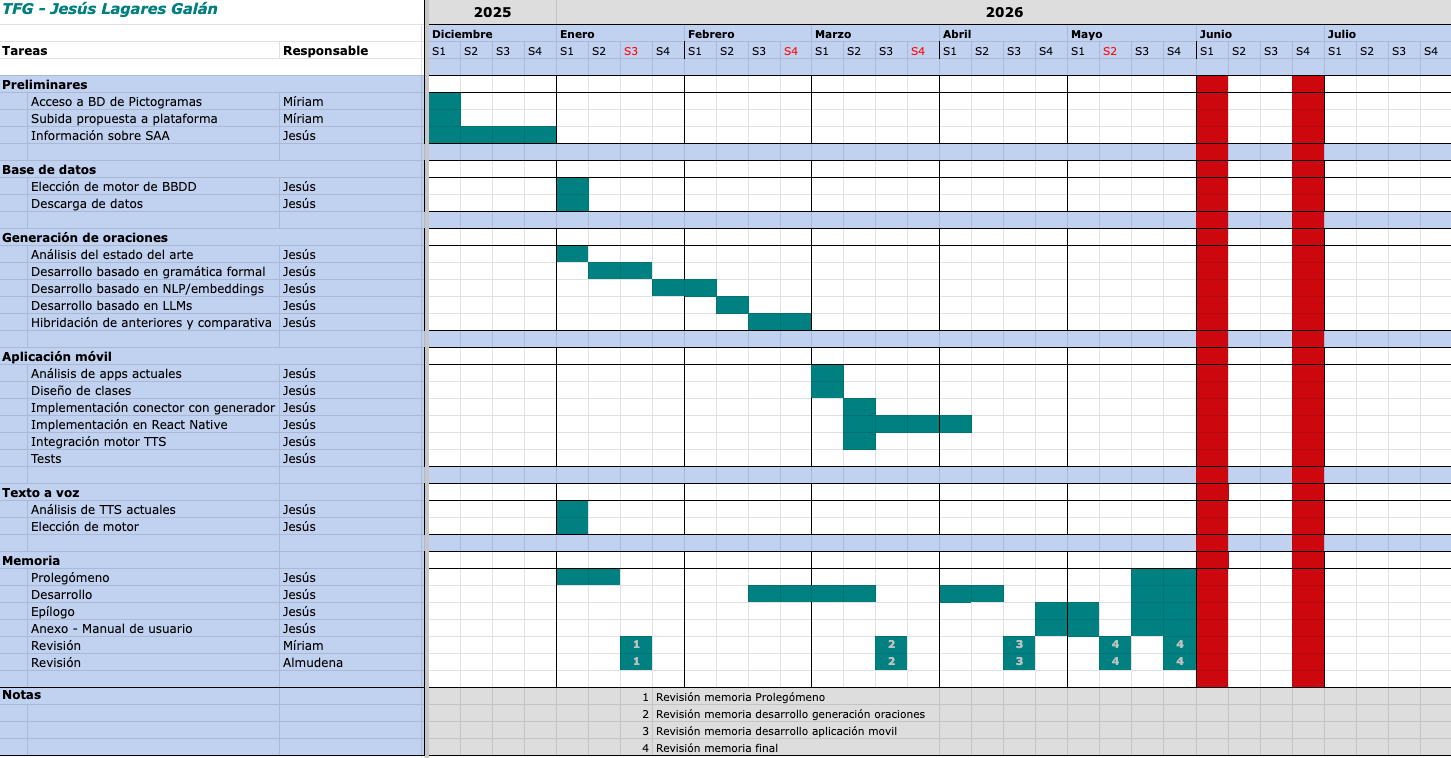
\includegraphics[width=\textwidth]{figures/gantt.png}
    \caption{Diagrama de Gantt con la planificación temporal del proyecto. Las franjas rojas marcan las dos convocatorias de defensa (junio y julio de 2026) y los números sobre las filas inferiores identifican los cuatro hitos de revisión de la memoria.}
    \label{fig:gantt}
\end{figure}

\section{Estimación de costes}
\label{sec:costes}

Al tratarse de un Trabajo de Fin de Grado, la estimación de costes se limita a los servicios externos que el sistema consume en ejecución. El trabajo del alumno, la supervisión de las tutoras y el equipo de desarrollo no se computan como gasto al formar parte de la dedicación académica propia del TFG, y el resto de herramientas empleadas son gratuitas o de código abierto.

La API de OpenAI~\cite{openai2024pricing} se utiliza en el motor de modelos de lenguaje y en las hibridaciones que lo incorporan. A precios de abril de 2026, GPT-4o factura \$2.50 por millón de tokens de entrada y \$10.00 por millón de salida, mientras que GPT-4o-mini se queda en \$0.15 y \$0.60 respectivamente; el desglose del coste por consulta aparece en la sección~\ref{ch:modelos-lenguaje}.

La API de ElevenLabs~\cite{elevenlabs2026pricing}, prevista para la síntesis de voz neuronal en la aplicación móvil, factura por caracteres: \$0.06 por cada 1.000 caracteres con los modelos \textit{Flash} y \textit{Turbo}, y \$0.12 con los modelos \textit{Multilingual v2} y \textit{v3}.

\section{Gestión de riesgos}
\label{sec:riesgos}

El desarrollo del proyecto está condicionado por cinco riesgos relevantes.

El tamaño del modelo de FastText utilizado por el enfoque de embeddings condiciona el despliegue. El modelo preentrenado sobre el corpus \textit{Spanish Billion Words} ocupa 6,7 GB en disco, lo que descarta funciones \textit{serverless} y servicios con restricciones de memoria. La mitigación consiste en desplegar el servidor mediante contenedores Docker con disco suficiente, lo que restringe la infraestructura pero no impide el funcionamiento.

La dependencia de la API de OpenAI afecta al motor de modelos de lenguaje y a las dos hibridaciones que lo incorporan: sin acceso a Internet, la mitad de las técnicas deja de operar. El servidor implementa \textit{fallback} automático a la gramática formal y a la gramática enriquecida con embeddings, que funcionan en local y permiten seguir dando servicio.

El vocabulario cerrado del sistema, limitado a 232 pictogramas de ARASAAC, deja fuera cualquier concepto no representado. La mitigación se abordó en la fase de selección, priorizando los conceptos más frecuentes en la comunicación cotidiana de usuarios de CAA y cubriendo nueve categorías semánticas.

La evaluación comparativa podría producir resultados inconcluyentes y comprometer las conclusiones del proyecto. Para minimizar este riesgo se combinan métricas automáticas (BLEU, ROUGE, BERTScore, perplejidad) con evaluación humana mediante encuestas, y se aplica el test de Wilcoxon~\cite{wilcoxon1945individual} con corrección para comparaciones múltiples, que permite discriminar qué diferencias entre técnicas son estadísticamente significativas.

La compatibilidad multiplataforma de la aplicación móvil introduce diferencias de comportamiento entre iOS y Android en renderizado, animaciones y acceso a APIs nativas. Se mitiga apoyándose en Expo como capa de abstracción, que unifica las APIs para la mayoría de funcionalidades que la aplicación necesita.

\section{Aseguramiento de la calidad}
\label{sec:calidad}

Las prácticas de aseguramiento de la calidad del proyecto abarcan cuatro niveles: verificación unitaria de los motores, evaluación comparativa automatizada, evaluación humana y verificación del servidor y la aplicación.

Los motores de generación de oraciones incorporan tests unitarios que verifican el comportamiento de cada componente de forma aislada: concordancias de género y número, inserción de determinantes y preposiciones, conjugación verbal, restricciones de selección semánticas e inferencia de elementos faltantes, entre otros. Estos tests permiten detectar regresiones cuando se modifican las reglas o los parámetros de los motores.

La evaluación comparativa automatizada constituye el segundo nivel de verificación. Un \textit{pipeline} ejecuta los seis motores sobre un conjunto de 130 casos de prueba y calcula para cada uno las métricas BLEU~\cite{papineni2002bleu}, ROUGE~\cite{lin2004rouge}, BERTScore~\cite{zhang2020bertscore} y perplejidad, entre otras. Los resultados se someten a tests de significancia estadística (Wilcoxon~\cite{wilcoxon1945individual} con corrección de Holm) para determinar si las diferencias entre técnicas son estadísticamente significativas. Los detalles de este proceso se describen en la sección~\ref{ch:evaluacion-comparativa}.

La evaluación humana complementa las métricas automáticas con la percepción de personas reales. Se diseñaron encuestas con escalas Likert de 7 puntos para medir la naturalidad percibida de las oraciones generadas y su proximidad a una referencia \textit{gold standard}. Este proceso, junto con sus resultados, se detalla en la sección~\ref{ch:evaluacion-comparativa}.

En la aplicación móvil, el uso de TypeScript como lenguaje de desarrollo proporciona tipado estático que detecta inconsistencias de tipos en tiempo de compilación. El servidor REST implementa \textit{endpoints} de salud (\textit{liveness} y \textit{readiness}) que permiten verificar automáticamente si el servicio está operativo y si los motores de generación están cargados y listos para procesar peticiones.



  
    % DESARROLLO
    \part{Desarrollo}
    \chapter{Introducción}
\label{ch:intro-generacion}
Antes de describir cada técnica de generación de lenguaje natural, conviene establecer el marco experimental que las tres comparten. Este capítulo define la arquitectura general del sistema, el conjunto de datos con el que se evalúan, las métricas que cuantifican su rendimiento y el entorno tecnológico en el que operan. De este modo, los capítulos siguientes pueden centrarse exclusivamente en las decisiones de diseño y los detalles de implementación de cada enfoque, sin repetir el contexto experimental.

\section{Descripción general del sistema}
\label{sec:descripcion-sistema}

El sistema Dixi transforma secuencias de pictogramas ARASAAC en oraciones naturales en español. Su arquitectura sigue un diseño modular donde la entrada ---una lista ordenada de etiquetas de pictogramas--- atraviesa un motor de generación de lenguaje natural y produce como salida una oración gramaticalmente correcta que, opcionalmente, un motor de síntesis de voz convierte en audio.

El aspecto central de este trabajo es el motor de generación. En lugar de implementar un único enfoque, se han desarrollado tres motores independientes que resuelven el mismo problema con técnicas de complejidad creciente:

\begin{itemize}
    \item La \textit{Fase 1} emplea una gramática formal extendida con restricciones de selección semánticas. Opera mediante pattern-matching sobre categorías gramaticales y reglas deterministas de inferencia contextual, sin dependencias externas de aprendizaje automático.
    \item La \textit{Fase 2} combina reglas gramaticales con embeddings de palabras. Utiliza vectores FastText para tomar decisiones semánticas ---como la predicción de preposiciones--- que una gramática puramente simbólica no puede resolver de forma general.
    \item La \textit{Fase 3} delega la generación lingüística a modelos de lenguaje grandes (GPT-4o y GPT-4o-mini) mediante ingeniería de prompts, prescindiendo de reglas explícitas.
\end{itemize}

Los tres motores reciben exactamente la misma entrada y producen el mismo tipo de salida, lo que permite una comparación directa. Esta progresión ---de lo simbólico a lo neuronal, de lo determinista a lo probabilístico--- no es casual: cada fase surge de las limitaciones observadas en la anterior y representa un compromiso diferente entre control, cobertura, coste y flexibilidad.

\section{Conjunto de datos de evaluación}
\label{sec:dataset}

La evaluación de los tres motores se realiza sobre un corpus de 115 casos de prueba diseñado específicamente para este proyecto. Cada caso consiste en una secuencia de pictogramas de entrada y la oración de referencia esperada como salida.

\subsection{Estructura y categorías}

Los 115 casos se distribuyen en ocho categorías semánticas que cubren los principales patrones comunicativos de un usuario de CAA:

\begin{table}[H]
\centering
\begin{tabular}{l l r}
\hline
Categoría & Descripción & Casos \\
\hline
Necesidad & Expresiones de deseo o necesidad & 25 \\
Movimiento & Desplazamiento a lugares & 15 \\
Estado & Estados físicos o emocionales & 15 \\
Descripción & Atributos de personas u objetos & 15 \\
Negativa & Oraciones con negación & 10 \\
Interrogativa & Preguntas con partícula interrogativa & 15 \\
Compuesta & Coordinación de elementos & 10 \\
Concordancia & Concordancia de género y número & 10 \\
\hline
\textit{Total} & & \textit{115} \\
\hline
\end{tabular}
\caption{Distribución de los casos de prueba por categoría semántica.}
\label{tab:dataset-categorias}
\end{table}

Cada categoría presenta desafíos lingüísticos específicos. Las oraciones de necesidad requieren inferir el verbo modal \textit{querer} cuando el usuario omite la intención; las de movimiento exigen seleccionar la preposición correcta según el lugar de destino; las interrogativas demandan invertir el orden sujeto-verbo; y las compuestas necesitan coordinación con conjunciones.

\subsection{Formato de los casos}

Cada caso de prueba se define como un par (entrada, referencia). La entrada es una lista de cadenas que representan las etiquetas de los pictogramas seleccionados por el usuario, y la referencia es la oración esperada en español natural. Por ejemplo:

\begin{lstlisting}[language={},caption={Ejemplo de caso de prueba del corpus de evaluación.}]
Entrada:    ["agua"]
Referencia: "Quiero agua"

Entrada:    ["yo", "querer", "comer", "manzana"]
Referencia: "Yo quiero comer una manzana"

Entrada:    ["donde", "estar", "mama"]
Referencia: "¿Donde esta mama?"
\end{lstlisting}

Nótese que la entrada puede variar en longitud desde un solo pictograma ---caso en el que el sistema debe inferir elementos omitidos--- hasta secuencias de cuatro o más pictogramas donde la tarea consiste principalmente en añadir los elementos funcionales (artículos, preposiciones, conjugaciones) que los pictogramas no codifican.

\subsection{Criterios de diseño del corpus}

El corpus se ha construido siguiendo tres criterios. En primer lugar, representatividad: las categorías reflejan las necesidades comunicativas más frecuentes de los usuarios de CAA, priorizando las expresiones de necesidad y deseo que constituyen la base de la comunicación funcional. En segundo lugar, gradualidad: dentro de cada categoría se incluyen casos de complejidad creciente, desde entradas mínimas que exigen máxima inferencia hasta secuencias completas donde el sistema solo debe aplicar morfología. En tercer lugar, cobertura gramatical: el conjunto abarca los principales fenómenos del español relevantes para CAA ---concordancia de género, contracciones, selección de preposiciones, interrogativas, negación y coordinación.

\section{Métricas de evaluación}
\label{sec:metricas}

Se emplean cinco métricas principales para evaluar la calidad de las oraciones generadas, complementadas con medidas de rendimiento operativo.

\subsection{Exact Match}

La métrica más estricta: compara la predicción con la referencia carácter a carácter, tras normalizar a minúsculas y eliminar espacios sobrantes. Devuelve 1 si la oración generada es idéntica a la referencia y 0 en cualquier otro caso. Su valor reside en que una coincidencia exacta garantiza corrección completa, pero su limitación es que penaliza por igual una variación menor (un artículo de más) y una oración completamente incorrecta.

$$\text{EM}(p, r) = \begin{cases} 1 & \text{si } \text{lower}(\text{strip}(p)) = \text{lower}(\text{strip}(r)) \\ 0 & \text{en otro caso} \end{cases}$$

\subsection{BLEU}

BLEU (\textit{Bilingual Evaluation Understudy}) mide la precisión de n-gramas entre la predicción y la referencia. Se calculan BLEU-1 (unigramas) y BLEU-4 (hasta 4-gramas), este último con suavizado +1 para evitar valores nulos en oraciones cortas donde no existen coincidencias de n-gramas de orden alto.

La precisión para n-gramas de orden $n$ se define como:

$$\text{precisión}_n = \frac{\text{coincidencias}_n + 1}{|\text{ngramas\_pred}_n| + 1}$$

El suavizado aditivo es necesario porque las oraciones de CAA son típicamente cortas (3-7 palabras), lo que hace frecuente la ausencia de 4-gramas compartidos incluso entre predicciones razonables.

BLEU-1 captura la adecuación léxica ---si las palabras correctas están presentes---, mientras que BLEU-4, al considerar secuencias más largas, refleja también la fluidez y el orden de las palabras. Ambas métricas se complementan: una predicción puede obtener BLEU-1 alto pero BLEU-4 bajo si contiene las palabras correctas en un orden incorrecto.

\subsection{ROUGE-L}

ROUGE-L se basa en la subsecuencia común más larga (\textit{Longest Common Subsequence}, LCS) entre la predicción y la referencia. A diferencia de BLEU, que requiere n-gramas consecutivos, ROUGE-L permite omisiones entre las palabras coincidentes, lo que la hace más tolerante con variaciones en el orden.

A partir de la longitud de la LCS se calculan precisión, recall y su media armónica $F_1$:

$$\text{precisión} = \frac{\text{LCS}}{|\text{pred}|}, \quad \text{recall} = \frac{\text{LCS}}{|\text{ref}|}$$

$$F_1 = \frac{2 \cdot \text{precisión} \cdot \text{recall}}{\text{precisión} + \text{recall}}$$

ROUGE-L resulta especialmente útil en este contexto porque captura la estructura secuencial de la oración sin penalizar la inserción de elementos adicionales (como artículos que el sistema añade correctamente pero que no figuran en la referencia de la misma forma).

\subsection{Cobertura}

La cobertura mide el porcentaje de casos del corpus para los que el sistema produce una salida válida, frente a los que rechaza o falla. Esta métrica es relevante porque la Fase 1, al operar con pattern-matching, solo puede procesar secuencias que coincidan con alguno de sus patrones sintácticos predefinidos, rechazando el resto.

$$\text{Cobertura} = \frac{\text{casos con salida válida}}{\text{total de casos}} \times 100$$

Las Fases 2 y 3, por su diseño, alcanzan cobertura del 100\%: la Fase 2 dispone de un mecanismo de fallback y la Fase 3 delega al LLM, que siempre genera alguna respuesta.

\subsection{BERTScore}

BERTScore evalúa la similitud semántica entre la predicción y la referencia utilizando embeddings contextuales de un modelo BERT. A diferencia de las métricas anteriores, que operan a nivel de tokens o n-gramas, BERTScore captura equivalencias semánticas ---por ejemplo, reconoce que \textit{deseo} y \textit{quiero} expresan significados cercanos aunque no compartan tokens.

Esta métrica se emplea exclusivamente en la evaluación de la Fase 3, donde el modelo de lenguaje puede generar paráfrasis válidas que las métricas de coincidencia exacta penalizarían. Para las Fases 1 y 2, cuyas salidas son deterministas y predecibles, las métricas de n-gramas resultan suficientes.

\subsection{Métricas operativas}

Además de la calidad lingüística, se miden dos aspectos operativos relevantes para un sistema de CAA:

\begin{itemize}
    \item \textit{Latencia}: tiempo de procesamiento por consulta, medido con temporizadores de alta resolución. En un sistema de comunicación, la latencia percibida por el usuario afecta directamente la fluidez de la interacción.
    \item \textit{Coste}: aplicable únicamente a la Fase 3, que utiliza una API comercial de pago. Se estima a partir del número de tokens procesados por consulta y las tarifas del proveedor.
\end{itemize}

\section{Entorno tecnológico}
\label{sec:entorno}

Los tres motores se implementan en Python 3.10+ y comparten la estructura de evaluación, pero difieren sustancialmente en sus dependencias:

\begin{table}[H]
\centering
\begin{tabular}{l l l}
\hline
Fase & Dependencias principales & Requisitos de hardware \\
\hline
Fase 1 & Ninguna (biblioteca estándar) & CPU \\
Fase 2 & FastText (modelo cc.es.300.bin, 4 GB) & CPU, 6 GB RAM \\
Fase 3 & API OpenAI (GPT-4o / GPT-4o-mini) & Conexión a Internet \\
\hline
\end{tabular}
\caption{Dependencias y requisitos por fase.}
\label{tab:dependencias}
\end{table}

La progresión en dependencias refleja un compromiso recurrente en el diseño del sistema: la Fase 1 funciona en cualquier entorno con Python instalado, la Fase 2 requiere descargar un modelo de embeddings de 4 GB y disponer de memoria suficiente para cargarlo, y la Fase 3 necesita conexión a Internet y una clave de API con coste asociado. Esta gradación en requisitos es relevante para el despliegue real en dispositivos de CAA, donde la conectividad no siempre está garantizada.

La evaluación se ejecuta en un entorno unificado para garantizar la comparabilidad: un equipo con procesador Apple M1, 16 GB de RAM y macOS, utilizando Python 3.12. Las mediciones de latencia se realizan en condiciones equivalentes, con la salvedad de que la Fase 3 incluye el tiempo de red de la llamada a la API.


\newpage{\ }
\cleardoublepage

\chapter{Gramática Formal}
\label{ch:gramatica-formal}
Una gramática formal es un conjunto de reglas que definen cómo se construyen las oraciones válidas de un lenguaje. En lingüística computacional, las gramáticas libres de contexto (CFG) describen la estructura sintáctica de las oraciones mediante reglas de producción que descomponen cada oración en constituyentes (sujeto, verbo, complemento) y estos a su vez en palabras. A partir de estas reglas, un sistema puede generar automáticamente oraciones correctas dada una entrada estructurada.

En este proyecto, la gramática formal se aplica al problema de CAA: dada una secuencia de pictogramas seleccionados por el usuario, las reglas de producción determinan qué tipo de oración construir (afirmativa, interrogativa, negativa), conjugan los verbos, insertan los artículos y preposiciones necesarios, y producen una oración gramaticalmente correcta en español. La gramática se ha extendido con restricciones de selección semánticas que verifican la compatibilidad entre verbos y argumentos (por ejemplo, que ``comer'' requiere un objeto comestible) y con reglas de inferencia contextual que completan la oración cuando la entrada del usuario es incompleta.

\section{Planteamiento del enfoque}
\label{sec:f1-planteamiento}

La decisión de comenzar con una gramática formal responde a una motivación práctica: establecer un modelo base determinista donde la misma entrada produce siempre la misma salida, facilitando la evaluación. Una gramática ofrece control total sobre la generación, ya que cada transformación lingüística está codificada explícitamente, e independencia de dependencias externas.

La filosofía de diseño prioriza la corrección gramatical sobre la cobertura: en un contexto de CAA, donde el usuario depende del sistema para comunicarse, es preferible rechazar una entrada no soportada a generar una frase incorrecta que distorsione su intención comunicativa.

El sistema no emplea una gramática libre de contexto (CFG) pura en el sentido de Chomsky~\cite{chomsky1957syntactic}. En lugar de reglas de producción clásicas del tipo $S \rightarrow NP\ VP$, implementa una CFG extendida mediante tres mecanismos complementarios.

La gramática se define formalmente con Lark~\cite{lark2024}, un \textit{toolkit} de \textit{parsing} para Python que acepta gramáticas en notación EBNF. Las producciones principales describen la jerarquía de tipos oracionales y las estructuras sintagmáticas que el sistema reconoce.

\begin{lstlisting}[caption={Producciones principales de la gramática CFG (notación EBNF/Lark).},label={lst:cfg-producciones},basicstyle=\ttfamily\small,xleftmargin=1cm]
oracion: oracion_compuesta | oracion_simple

oracion_simple: oracion_interrogativa
              | oracion_negativa
              | oracion_afirmativa

oracion_afirmativa: oracion_necesidad | oracion_accion
                  | oracion_estado | oracion_descripcion
                  | oracion_locativa

oracion_necesidad: sujeto? verbo_necesidad complemento_necesidad
oracion_accion:    sujeto? verbo_accion complemento_verbal?
oracion_estado:    sujeto? verbo_estado predicado_estado
oracion_descripcion: sujeto verbo_copulativo predicado_descripcion
oracion_locativa:  sujeto? verbo_movimiento sintagma_preposicional

oracion_negativa:  NEGACION oracion_afirmativa

oracion_interrogativa: pregunta_con_interrogativo
                     | pregunta_si_no

oracion_compuesta: oracion_temporal | oracion_coordinada
oracion_temporal:  marcador_temporal oracion_simple
oracion_coordinada: oracion_simple conjuncion oracion_simple

sintagma_nominal:       determinante? sustantivo adjetivo?
sintagma_preposicional: preposicion sintagma_nominal
objeto_con_modificador: determinante? objeto adjetivo?
\end{lstlisting}

La gramática completa incluye además las definiciones de los terminales léxicos (pronombres, verbos por subcategoría, objetos, lugares, personas, adjetivos, interrogativos, marcadores temporales y modificadores), que en conjunto conforman las 646 entradas del léxico descrito en la sección~\ref{sec:f1-lexico}.

Lark permitió especificar estas reglas de forma declarativa y verificar su coherencia, pero el motor de generación no utiliza el \textit{parser} Earley ni el árbol de sintaxis que Lark produce. Las entradas de CAA son secuencias cortas (entre una y cinco palabras) extraídas de un vocabulario cerrado de 232 pictogramas, lo que hace que el conjunto de patrones válidos sea finito y enumerable. En este escenario, un \textit{parser} formal resulta sobredimensionado: la implementación traduce la gramática a 48 patrones sintácticos codificados como secuencias de categorías gramaticales y los reconoce por \textit{matching} directo. El resultado es más simple de depurar, determinista por construcción y suficiente para la complejidad del dominio.

Los tres mecanismos que extienden la CFG operan sobre estos patrones. El \textit{pattern-matching} sobre categorías gramaticales define cada patrón sintáctico como una secuencia ordenada de categorías (por ejemplo, verbo de necesidad seguido de verbo de acción y objeto), y se selecciona el primer patrón que coincide con la clasificación categorial de la entrada. Las restricciones de selección semánticas~\cite{resnik1996selectional} validan que los argumentos de cada verbo cumplan rasgos específicos (``comer'' requiere un objeto comestible, ``ir'' requiere un complemento de lugar). Las reglas de inferencia contextual completan la oración cuando la entrada del usuario es incompleta: por ejemplo, la entrada ``agua'' activa la inferencia del verbo ``quiero'', produciendo ``Quiero agua''.

Esta combinación permite manejar la ambigüedad inherente a la entrada abreviada de CAA sin recurrir a modelos estadísticos o neuronales.

\section{Decisiones de diseño específicas}
\label{sec:f1-postprocesamiento}

El postprocesador transforma la secuencia tokenizada en una oración natural. Tres de sus etapas incorporan decisiones de diseño específicas de este proyecto que van más allá de lo que una gramática formal estándar resolvería.

\subsection{Inferencia de elementos faltantes}

Esta etapa detecta elementos implícitos en la entrada del usuario y los añade explícitamente, siguiendo reglas que priorizan la inferencia conservadora:

\begin{itemize}
    \item Un solo objeto (``agua'') activa la inserción de ``quiero''.
    \item Un solo lugar (``baño'') activa la inserción de ``quiero'' e ``ir''.
    \item Un infinitivo sin verbo modal (``comer manzana'') recibe ``quiero'' como prefijo.
\end{itemize}

La inferencia opera exclusivamente en primera persona y no se activa en interrogativas, evitando asumir la intención del usuario cuando pregunta sobre terceros. Esta lógica es específica del dominio de CAA: en la comunicación aumentativa, el usuario selecciona los pictogramas mínimos necesarios y el sistema debe completar la intención comunicativa implícita.

\subsection{Inserción de determinantes}

La decisión de qué determinante acompaña a cada sustantivo depende de reglas específicas del dominio. Los sustantivos incontables (agua, pan, leche) no reciben determinante tras verbos de necesidad. Los objetos con artículo definido (televisión, teléfono, música) usan ``el/la'' en lugar de ``un/una''. En interrogativas se utiliza artículo definido (``¿Dónde está el perro?''). En coordinaciones, la coherencia entre los miembros determina el tratamiento: si un elemento es incontable, el otro también omite el determinante.

\subsection{Inserción de preposiciones}

La selección de la preposición correcta para complementos de lugar utiliza tres diccionarios construidos manualmente: preposiciones por verbo de movimiento (9 verbos: ``ir'' $\rightarrow$ ``a'', ``venir'' $\rightarrow$ ``de''), preposiciones por lugar con verbos de movimiento (35 lugares: ``baño'' $\rightarrow$ ``al'', ``escuela'' $\rightarrow$ ``a la'') y preposiciones de ubicación para verbos de estado (19 lugares: ``colegio'' $\rightarrow$ ``en el''). La lógica busca hacia atrás desde el lugar hasta encontrar el verbo que lo rige, y selecciona el diccionario apropiado según el tipo de verbo.

\section{Limitaciones}
\label{sec:f1-limitaciones}

Las gramáticas formales presentan limitaciones inherentes al enfoque simbólico. En primer lugar, operan sobre un vocabulario cerrado: toda palabra no incluida en el léxico se rechaza, lo que impide al sistema adaptarse a vocabulario nuevo sin intervención manual. En segundo lugar, las reglas de producción capturan la estructura sintáctica pero no el significado ni el contexto pragmático: una gramática no puede distinguir entre dos oraciones sintácticamente idénticas pero semánticamente diferentes, ni resolver ambigüedades que dependen del contexto comunicativo. En tercer lugar, la cobertura lingüística depende enteramente de las reglas codificadas: cada nueva estructura oracional, tiempo verbal o fenómeno morfológico requiere añadir reglas explícitamente, un esfuerzo de mantenimiento que crece con la complejidad del dominio. Por último, y quizá la limitación más relevante, las reglas son específicas de un idioma y un dominio concretos: las decisiones sobre inferencia de verbos modales, selección de preposiciones o inserción de determinantes están codificadas para el español y para el vocabulario de CAA de este proyecto. Extender el sistema a otro idioma o a un dominio comunicativo diferente requeriría reescribir la práctica totalidad de las reglas, ya que ninguna de ellas es transferible. Esta falta de portabilidad es inherente a las gramáticas formales aplicadas a la generación de lenguaje natural, y es precisamente lo que motiva y justifica la exploración de técnicas complementarias (embeddings semánticos, modelos de lenguaje) que puedan generalizar más allá del dominio para el que fueron diseñadas.


\newpage{\ }
\cleardoublepage

\chapter{Gramática Formal Enriquecida con Embeddings}
\label{ch:enfoque-hibrido}
La segunda técnica surge de una limitación concreta de la gramática formal: su cobertura del 88,46\% implica que una de cada nueve entradas no produce salida alguna. Este capítulo describe un enfoque híbrido que combina reglas gramaticales con embeddings de palabras para superar ese techo sin abandonar el control sobre la generación.

\section{Planteamiento del enfoque}
\label{sec:f2-planteamiento}

La motivación para esta segunda fase es precisa: la gramática formal alcanza el 100\% de Exact Match en los casos que reconoce, pero rechaza toda entrada cuya secuencia de categorías no coincida con alguno de sus 46 patrones predefinidos. Ampliar la cobertura añadiendo más patrones es posible pero no escalable ---cada nuevo patrón comunicativo exige definir explícitamente su regla, y la combinatoria de posibles secuencias crece rápidamente---.

La solución adoptada es una arquitectura híbrida que asigna cada decisión lingüística al mecanismo más adecuado para ella. Las reglas gramaticales se encargan de las operaciones deterministas: conjugación verbal, selección de artículos, contracciones y concordancia de género. Los embeddings semánticos intervienen en las decisiones que dependen del significado y que una gramática simbólica no puede resolver de forma general: la predicción de preposiciones (¿\textit{ir al colegio} o \textit{ir en el colegio}?), la validación de combinaciones verbo-argumento y la clasificación de roles semánticos.

Antes de llegar a este diseño se exploró y descartó un enfoque de recuperación semántica (\textit{retrieval}). Dado un conjunto de pictogramas, el sistema buscaba en el corpus de referencia la frase cuya representación vectorial fuese más similar a la composición de los embeddings de entrada. Este enfoque fue abandonado porque el corpus de evaluación era la misma fuente de la que se recuperaban las frases, produciendo métricas artificialmente infladas que no reflejaban capacidad real de generalización: el sistema no generaba frases sino que las copiaba.

\section{Modelo de embeddings}
\label{sec:f2-embeddings}

El sistema utiliza el modelo preentrenado FastText \texttt{cc.es.300.bin}, entrenado sobre Common Crawl en español. Cada palabra se representa como un vector de 300 dimensiones, y la similitud entre palabras se mide mediante similitud coseno.

La elección de FastText frente a alternativas como Word2Vec, GloVe o BERT responde a una ventaja crítica para el español: el manejo nativo de palabras fuera de vocabulario (\textit{out-of-vocabulary}, OOV). FastText representa cada palabra como la suma de los vectores de sus n-gramas de caracteres, lo que permite generar embeddings razonables para formas morfológicas no vistas durante el entrenamiento ---conjugaciones, diminutivos, formas de género--- sin necesidad de un vocabulario exhaustivo. Word2Vec y GloVe carecen de esta capacidad, devolviendo un vector nulo para cualquier palabra no presente en su vocabulario. BERT ofrece embeddings contextuales superiores pero su latencia ($\sim$50 ms por consulta frente a $\sim$0,01 ms de FastText) y sus dependencias (PyTorch, GPU recomendada) no se justifican para un sistema de consulta puntual sobre palabras individuales.

Para representar una secuencia de pictogramas como un único vector, el sistema implementa tres estrategias de composición vectorial: promedio simple, promedio ponderado ---donde las palabras de contenido reciben peso 1,0 y las palabras funcionales 0,3--- y SIF (\textit{Smooth Inverse Frequency}), que pondera cada palabra inversamente a su frecuencia estimada en el idioma. La estrategia utilizada por defecto es el promedio ponderado, que equilibra sencillez y sensibilidad al contenido semántico relevante.

\section{Léxico}
\label{sec:f2-lexico}

El léxico de esta fase contiene 355 entradas exportadas directamente desde la Fase 1 mediante un script de conversión. Cada entrada se almacena como un objeto JSON con campos que varían según la categoría: los verbos incluyen conjugaciones completas por pronombre, los lugares incluyen preposiciones de movimiento y ubicación, los adjetivos incluyen formas de género, y los objetos incluyen rasgos como \texttt{uncountable} y \texttt{definite\_article}.

La decisión de reutilizar el léxico de la Fase 1 ---en lugar de construir uno independiente--- responde a tres razones: la información lingüística ya estaba validada, se garantiza consistencia entre ambas fases al evaluar sobre el mismo conjunto de conceptos, y se evita duplicar un esfuerzo considerable de etiquetado manual. El script de exportación (\texttt{export\_lexicon.py}) importa las clases de la Fase 1, itera sobre todas las categorías de palabras, genera las conjugaciones verbales y enriquece las entradas con información adicional del postprocesador (sustantivos incontables, artículos definidos, preposiciones por lugar). La diferencia fundamental con el léxico de la Fase 1 es el formato: mientras que aquella lo codifica como estructuras Python en memoria, esta fase lo serializa a JSON para independizar el léxico del código.

\section{Analizador semántico}
\label{sec:f2-analizador}

El analizador semántico es el módulo central del sistema, con 608 líneas que constituyen el componente más complejo. Su función es transformar una lista de etiquetas de pictogramas en un análisis estructurado que contenga el sujeto, los verbos, los argumentos con sus roles semánticos, las preposiciones predichas y los modificadores.

El análisis se realiza en ocho pasadas secuenciales sobre la entrada.

\subsection{Clasificación de pictogramas}

La primera pasada clasifica cada pictograma consultando el léxico y los índices de búsqueda. El sistema mantiene tres índices: un mapa directo palabra $\rightarrow$ entrada léxica, un mapa de formas de género (\textit{bonita} $\rightarrow$ \textit{bonito}) y un mapa inverso de conjugaciones (\textit{quiero} $\rightarrow$ \textit{querer}). Para palabras ambiguas ---como \textit{cocina}, que puede ser verbo o lugar, o \textit{ayuda}, que puede ser verbo o sustantivo--- el sistema aplica conjuntos de \textit{overrides} que fuerzan la clasificación correcta según el contexto de CAA.

\subsection{Detección de sujetos}

La segunda pasada identifica el sujeto de la oración. Los pronombres se reconocen directamente; para sujetos no pronominales (personas como \textit{mamá} o \textit{papá}), el sistema verifica que la palabra preceda a un verbo copulativo o de estado, lo que indica función de sujeto y no de complemento.

\subsection{Inferencia de elementos implícitos}

La tercera pasada implementa la inferencia de elementos que el usuario omite. Cuando la entrada contiene solo objetos o lugares sin verbos, el sistema inserta \textit{querer} y, si hay lugares, también \textit{ir}. Esta inferencia opera exclusivamente en primera persona y se desactiva en oraciones interrogativas, evitando asumir la intención del usuario cuando pregunta sobre terceros. La lógica es más conservadora que la de la Fase 1: al disponer de embeddings para resolver ambigüedades, el sistema puede permitirse inferir menos elementos y delegar más decisiones al análisis semántico.

\subsection{Asignación de roles verbales y clasificación de argumentos}

Las pasadas cuarta a sexta determinan la categoría del verbo principal, identifican la persona gramatical en interrogativas, y clasifican los argumentos restantes (sustantivos, adjetivos, lugares) según su función sintáctica. La clasificación de argumentos distingue entre objetos directos, complementos de lugar, adjetivos atributivos y sustantivos de estado, utilizando tanto la categoría léxica como, cuando es ambigua, la similitud de embeddings entre el verbo y el argumento candidato.

\subsection{Desambiguación de roles y predicción de preposiciones}

La séptima pasada resuelve las asignaciones ambiguas de roles y predice las preposiciones. Para cada argumento clasificado como complemento, el sistema aplica un predictor de preposiciones de tres niveles (descrito en la sección siguiente). Para la desambiguación de roles, compara la similitud coseno entre el verbo y cada argumento candidato, asignando el rol de objeto directo al más similar y los restantes como complementos preposicionales.

\subsection{Coordinación}

La octava pasada detecta y procesa la coordinación de elementos: objetos coordinados (\textit{agua y pan}), verbos coordinados (\textit{comer y beber}) y adjetivos coordinados. La presencia de una conjunción en la entrada activa esta pasada, que agrupa los elementos coordinados para que la plantilla los trate como una unidad.

\section{Predicción de preposiciones}
\label{sec:f2-preposiciones}

La predicción de preposiciones es una de las contribuciones principales del componente de embeddings. El sistema implementa un predictor de tres niveles con degradación progresiva de confianza.

\subsection{Nivel 1: reglas por lugar}

Cuando el sustantivo es un lugar con preposiciones codificadas en el léxico, el sistema aplica directamente la regla. Si el verbo es de movimiento, utiliza la preposición de movimiento del lugar (\textit{ir al colegio}); si no lo es, utiliza la de ubicación (\textit{estar en el colegio}). La confianza de este nivel es 1,0.

\subsection{Nivel 2: prototipos vectoriales}

Si no existe regla de lugar, el sistema recurre a prototipos vectoriales construidos offline a partir del corpus SBWCE (\textit{Spanish Billion Word Corpus and Embeddings}). Para cada preposición, el prototipo es la media de los vectores de contexto (suma de embedding del verbo y del sustantivo) extraídos de las tripletas \textit{(palabra\_antes, preposición, palabra\_después)} del corpus:

$$\vec{p}_k = \frac{1}{|C_k|} \sum_{(w_a, w_d) \in C_k} (\vec{w}_a + \vec{w}_d)$$

En tiempo de ejecución, dado un par (verbo, sustantivo), se calcula el vector de contexto $\vec{c} = \vec{v} + \vec{n}$ y se selecciona la preposición cuyo prototipo tiene mayor similitud coseno con $\vec{c}$, siempre que supere un umbral mínimo de confianza (0,15). Los prototipos se calculan una sola vez y se almacenan en caché como un archivo JSON.

\subsection{Nivel 3: reglas por verbo}

Como fallback final, si los prototipos no superan el umbral, el sistema consulta la preposición por defecto del verbo codificada en el léxico (\textit{ir} $\rightarrow$ \textit{a}, \textit{venir} $\rightarrow$ \textit{de}).

Este diseño de tres niveles ejemplifica la filosofía híbrida del sistema: las reglas codificadas cubren los casos conocidos con certeza, los embeddings extienden la cobertura a combinaciones no anticipadas, y un fallback determinista garantiza que siempre se produce alguna salida.

\section{Selector de plantillas y realizador morfológico}
\label{sec:f2-plantillas}

Una vez completado el análisis semántico, el selector de plantillas evalúa el resultado contra 15 plantillas sintácticas y selecciona la más específica que se ajusta a los elementos presentes. Las plantillas están ordenadas por especificidad descendente: \texttt{S\_Vmodal\_Vinf\_OD} (sujeto + verbo modal + infinitivo + objeto directo, como \textit{Yo quiero comer una manzana}) tiene prioridad sobre \texttt{SVO} (sujeto + verbo + objeto, como \textit{Yo como una manzana}), que a su vez tiene prioridad sobre \texttt{VO} (verbo + objeto, como \textit{Quiero agua}). La plantilla \texttt{FALLBACK} actúa como último recurso, concatenando las palabras sin estructura sintáctica.

El realizador morfológico rellena los slots de la plantilla seleccionada con las formas flexionadas correctas. Conjuga el verbo principal según la persona del sujeto, selecciona el artículo apropiado para cada sustantivo (indefinido, definido o ausente según las propiedades del léxico), aplica las contracciones (\textit{a el} $\rightarrow$ \textit{al}), resuelve la concordancia de género de los adjetivos y capitaliza la primera letra. Para interrogativas, invierte el orden sujeto-verbo y envuelve la oración con los signos \textit{¿...?}.

\section{Organización del código}
\label{sec:f2-codigo}

El sistema se implementa en nueve módulos Python, con FastText como única dependencia de aprendizaje automático.

\begin{table}[H]
\centering
\begin{tabular}{l r l}
\hline
Módulo & Líneas & Propósito \\
\hline
\texttt{semantic\_analyzer.py} & 608 & Análisis semántico en 8 pasadas \\
\texttt{vector\_composer.py} & 181 & 3 estrategias de composición vectorial \\
\texttt{morphological\_realizer.py} & 170 & Conjugación, artículos, concordancia \\
\texttt{preposition\_builder.py} & 154 & Prototipos vectoriales desde corpus \\
\texttt{hybrid\_generator.py} & 139 & Orquestador del pipeline \\
\texttt{template\_selector.py} & 130 & 15 plantillas sintácticas \\
\texttt{text\_preprocessor.py} & 107 & Normalización y tokenización \\
\texttt{config.py} & 65 & Constantes y umbrales \\
\texttt{embedding\_loader.py} & 48 & Interfaz con FastText \\
\texttt{similarity\_engine.py} & 55 & Similitud coseno individual y batch \\
\hline
\end{tabular}
\caption{Estructura del código del motor híbrido.}
\label{tab:f2-codigo}
\end{table}

Las dependencias fluyen de arriba hacia abajo: \texttt{config.py} proporciona constantes globales, \texttt{embedding\_loader.py} encapsula el acceso a FastText, \texttt{semantic\_analyzer.py} es el módulo central que combina léxico y embeddings, y \texttt{hybrid\_generator.py} orquesta todos los componentes. La separación entre análisis semántico, selección de plantilla y realización morfológica permite modificar cualquiera de las tres etapas de forma independiente.

\section{Resultados}
\label{sec:f2-resultados}

La evaluación sobre el corpus de 115 casos arroja los resultados que muestra la Tabla~\ref{tab:f2-resultados}.

\begin{table}[H]
\centering
\begin{tabular}{l r}
\hline
Métrica & Valor \\
\hline
Cobertura & 100\% (115 de 115) \\
Exact Match global & Variable por categoría \\
BLEU-1 corpus & 0,8846 \\
BLEU-4 corpus & 0,6653 \\
ROUGE-L $F_1$ & 0,9035 \\
Latencia media & $<$1 ms (sin carga de modelo) \\
\hline
\end{tabular}
\caption{Resultados del motor híbrido con embeddings.}
\label{tab:f2-resultados}
\end{table}

El resultado más significativo es la cobertura del 100\%: todas las entradas producen una salida, frente al 88,46\% de la Fase 1. Este salto se debe al mecanismo de fallback y a la capacidad del analizador semántico de procesar secuencias que no encajan en patrones rígidos. Sin embargo, la cobertura total no implica corrección total ---el Exact Match varía según la categoría, siendo más bajo en casos donde la predicción de preposiciones o la asignación de roles introduce variaciones respecto a la referencia---.

La comparación directa con la Fase 1 revela un compromiso entre cobertura y precisión puntual. La gramática formal era perfecta dentro de su dominio (100\% EM en casos parseables) pero rechazaba el 11,54\% de las entradas; el enfoque híbrido cubre todas las entradas pero comete errores en algunas de ellas. Esta tensión entre cobertura y exactitud motiva la exploración de una tercera vía ---los modelos de lenguaje--- que promete combinar la cobertura total con una capacidad de generalización lingüística que ni las reglas ni los embeddings alcanzan por sí solos.


\newpage{\ }
\cleardoublepage

\chapter{Modelos de Lenguaje}
\label{ch:modelos-lenguaje}
La tercera y última técnica abandona las reglas explícitas y delega la generación lingüística a modelos de lenguaje grandes.

Este capítulo describe cómo se guía un LLM comercial mediante ingeniería de prompts~\cite{brown2020language} para resolver el mismo problema que los dos motores anteriores abordaron con gramáticas y embeddings.

\section{Diseño del prompt}
\label{sec:f3-prompt}

La ingeniería de prompts es el componente central de este motor. A diferencia de un modelo ajustado (\textit{fine-tuned})~\cite{brown2020language}, toda la adaptación al dominio CAA se codifica en el prompt enviado en cada llamada a la API.

\subsection{System prompt}

El \textit{system prompt} define el rol del modelo como motor de lenguaje de una aplicación CAA y establece once reglas estrictas que gobiernan la generación (véase Extracto de código~\ref{lst:system-prompt} del Anexo~\ref{anx:codigo}). Las reglas cubren cuatro aspectos.

La \textit{fidelidad semántica} (regla 1) es la restricción más importante: la oración debe expresar exactamente el significado de los pictogramas proporcionados, sin añadir información ni conceptos ausentes en la entrada. En un contexto CAA, generar contenido no seleccionado por el usuario equivaldría a poner en su boca palabras que no ha elegido.

Los \textit{elementos funcionales} (regla 2) especifican qué puede añadir el modelo: artículos, preposiciones de enlace, conjugación verbal y concordancia de género. Estas son las mismas operaciones que los motores anteriores resolvían con reglas explícitas (sección~\ref{sec:f1-postprocesamiento}); aquí se delegan al LLM mediante una instrucción textual.

El \textit{formato y registro} (reglas 3-5, 8, 10) restringe la salida a una única oración en registro coloquial-neutro, sin explicaciones ni alternativas. Sin estas restricciones, los LLMs frecuentemente producen texto adicional como ``Aquí tienes la oración:'' o generan múltiples variantes.

Las \textit{reglas lingüísticas} (reglas 6-7, 9, 11) cubren fenómenos específicos: interrogativas con signos ¿...?, posición de la negación, omisión del pronombre sujeto (\textit{pro-drop} del español) y concordancia de género. La regla 11, sobre concordancia, fue añadida respecto al diseño original para cubrir la categoría de concordancia del dataset de evaluación.

\subsection{Ejemplos few-shot}

Las reglas del \textit{system prompt} describen qué debe hacer el modelo, pero no le muestran cómo hacerlo. Sin ejemplos concretos, el modelo tiende a interpretar las instrucciones de forma demasiado literal o demasiado libre, produciendo salidas que cumplen las reglas individualmente pero no capturan el registro ni la brevedad esperados en CAA.

El motor utiliza 15 ejemplos \textit{few-shot}~\cite{brown2020language} que cubren las ocho categorías del dataset. Cada ejemplo es un par (pictogramas de entrada, oración esperada) que se inyecta como intercambio usuario-asistente en el historial de mensajes.

\begin{table}[H]
\centering
\begin{tabular}{r l l l}
\hline
\# & Categoría & Pictogramas & Oración \\
\hline
1 & Necesidad & quiero + agua & Quiero agua \\
2 & Necesidad & necesito + dormir & Necesito dormir \\
3 & Necesidad & quiero + comer + manzana & Quiero comer una manzana \\
4 & Inferencia & agua & Quiero agua \\
5 & Movimiento & ir + baño & Quiero ir al baño \\
6 & Estado & estoy + cansado & Estoy cansado \\
7 & Estado & tengo + hambre & Tengo hambre \\
8 & Descripción & perro + es + grande & El perro es grande \\
9 & Interrogativa & dónde + estar + mamá & ¿Dónde está mamá? \\
10 & Interrogativa & qué + comer & ¿Qué comes? \\
11 & Negación & no + quiero + dormir & No quiero dormir \\
12 & Negación & no + tengo + hambre & No tengo hambre \\
13 & Compuesta & agua + y + pan & Quiero agua y pan \\
14 & Compuesta & mañana + ir + colegio & Mañana quiero ir al colegio \\
15 & Concordancia & quiero + manzana + rojo & Quiero una manzana roja \\
\hline
\end{tabular}
\caption{Los 15 ejemplos \textit{few-shot} del motor de modelos de lenguaje.}
\label{tab:f3-fewshot}
\end{table}

El número de 15 se fijó porque es el mínimo que cubre las ocho categorías del dataset con al menos un ejemplo representativo; añadir más ejemplos incrementaría el coste de cada llamada sin beneficio proporcional, dado que los aproximadamente 1.204 tokens de entrada ya están dominados por el prompt fijo y los \textit{few-shot} existentes.

Los criterios de selección priorizan la cobertura de patrones que requieren inferencia: el ejemplo 4 enseña al modelo a expandir un solo sustantivo en una oración de necesidad; el ejemplo 5, a insertar la preposición contraída \textit{al}; el ejemplo 15, a corregir la concordancia de género. Los ejemplos se adaptaron al formato real del dataset, que utiliza tanto infinitivos como formas conjugadas como pictogramas de entrada.

\subsection{Construcción dinámica del prompt}

Cada mensaje de usuario formatea los pictogramas incluyendo su categoría gramatical entre paréntesis (por ejemplo, \texttt{Pictogramas: quiero (verbo modal) + agua (sustantivo)}).

Esta información desambiguadora procede del inventario de metadatos y ayuda al modelo a interpretar correctamente pictogramas polisémicos: ``como'' puede ser verbo (primera persona de ``comer'') o interrogativo (``¿cómo?''), y la categoría aclara la interpretación esperada.

Cada llamada consume aproximadamente 1.204 tokens de entrada, de los cuales la gran mayoría corresponden al \textit{system prompt} y los ejemplos \textit{few-shot}. La consulta del usuario aporta típicamente 10-20 tokens adicionales. Los tokens de salida son muy reducidos: 4 tokens en promedio, coherente con la brevedad de las oraciones de CAA.

\section{Metadatos de pictogramas}
\label{sec:f3-metadatos}

La temperatura de 0.3 prioriza la consistencia sobre la creatividad: en CAA, la variabilidad no aporta valor y la predecibilidad es deseable. Una temperatura de 0 sería completamente determinista, pero 0.3 permite cierta flexibilidad para manejar construcciones no vistas en los \textit{few-shot}.

El límite de 100 tokens es generoso para oraciones que promedian 4 tokens de salida, pero actúa como salvaguarda contra generaciones desbordadas. El timeout de 10 segundos refleja que, en una aplicación de comunicación asistida, el usuario espera activamente la respuesta.

El cliente implementa reintentos diferenciados según el tipo de error (véase Extracto de código~\ref{lst:llm-client} del Anexo~\ref{anx:codigo}): los errores de \textit{rate limit} se reintentan con backoff exponencial (2 y 4 segundos), los timeouts se reintentan inmediatamente, y los errores de servidor no se reintentan.

El coste se estima a partir de los precios de la API~\cite{openai2024pricing}: \$2.50/1M tokens de entrada y \$10.00/1M de salida para GPT-4o, frente a \$0.15/1M y \$0.60/1M para GPT-4o-mini.

Con los aproximadamente 1.204 tokens de entrada y 4 de salida descritos en la sección~\ref{sec:f3-prompt}, cada consulta cuesta \$0.00018 con GPT-4o-mini y \$0.00305 con GPT-4o, una diferencia de factor 16.7$\times$.

\section{Validación post-generación}
\label{sec:f3-validacion}

A diferencia de los motores basados en reglas, donde la corrección de la salida es consecuencia directa de las reglas aplicadas, un LLM puede producir respuestas vacías, omitir pictogramas de la entrada o ignorar instrucciones del prompt. En el contexto de CAA, donde el usuario depende del sistema para comunicarse, una salida que no refleje los pictogramas seleccionados es un fallo funcional. Por este motivo, el motor incorpora un validador específico que verifica dos aspectos que los LLMs no garantizan por diseño.

El primero es la cobertura de conceptos: el validador comprueba que cada pictograma seleccionado por el usuario esté representado en la oración generada, teniendo en cuenta las variaciones morfológicas del español (el pictograma ``querer'' puede aparecer como ``quiero'' o ``quiere'' en la salida). El segundo es el formato interrogativo: cuando la entrada contiene un pictograma interrogativo, se verifica que la respuesta incluya los signos de interrogación correspondientes, una convención ortográfica del español que el modelo no siempre respeta.

\section{Limitaciones}
\label{sec:f3-limitaciones}

El motor depende de la API de OpenAI, lo que implica conexión a Internet permanente y un servicio de pago que no es viable para uso offline. La latencia de red añade aproximadamente un segundo a cada generación, un tiempo perceptible en una aplicación de comunicación asistida.

Aunque el coste por consulta es reducido (\$0.00018 con GPT-4o-mini)~\cite{openai2024pricing}, el uso continuado genera un gasto acumulativo que no existe en los motores simbólicos.

Con temperatura 0.3, la misma entrada puede producir salidas ligeramente diferentes entre ejecuciones, lo que dificulta la depuración y la reproducibilidad de los resultados.

Las interrogativas son la categoría más difícil para el modelo, con las dos únicas interrogativas de los 15 ejemplos \textit{few-shot} insuficientes para cubrir la variedad de inferencias de persona verbal que esta categoría requiere.


\newpage{\ }
\cleardoublepage

\chapter{Técnicas de Hibridación}
\label{ch:hibridacion}
Los capítulos anteriores han mostrado que cada técnica de generación tiene fortalezas y carencias complementarias. Las gramáticas formales producen salidas correctas y predecibles, pero rígidas y limitadas a las estructuras previstas. Los embeddings añaden información semántica pero no alteran la estructura de la generación. Los LLMs producen texto natural y flexible, pero sin garantías de fidelidad al contenido de entrada y con dependencia de infraestructura externa.

La hibridación parte de la hipótesis de que combinar estas técnicas puede producir resultados superiores a los de cada una por separado: una gramática que garantice la estructura, enriquecida con la naturalidad de un LLM, o un sistema que genere múltiples candidatos y seleccione el mejor. Se implementan tres estrategias de hibridación con objetivos diferenciados. Las dos primeras se basan en el patrón \textit{plan-then-realize}~\cite{moryossef2019stepbystep} y en la post-edición neuronal de texto generado por reglas~\cite{chen2025axsemantics}. La tercera implementa el paradigma de sobregeneración y ranking~\cite{sharma2019overgenerate}. Los resultados de la evaluación comparativa (capítulo~\ref{ch:evaluacion-comparativa}) permitirán determinar si esta hipótesis se confirma en la práctica.

\textit{(TODO: Añadir diagrama de arquitectura mostrando los tres pipelines y cómo reutilizan los motores existentes.)}

\section{Hibridación 1: Gramática + LLM como post-editor}
\label{sec:h-hybrid1}

Las Hibridaciones 1 y 2 se basan en dos patrones complementarios. El primero es el uso de un LLM como post-editor de sistemas de reglas, documentado por Chen et al.~\cite{chen2025axsemantics} en un sistema de producción de AX Semantics: el sistema de reglas garantiza la estructura y la fidelidad al contenido, mientras que el LLM aporta fluidez y naturalidad. El segundo es el patrón \textit{plan-then-realize}~\cite{moryossef2019stepbystep}, que separa la generación en un planificador simbólico que decide qué decir y un realizador neural que lo transforma en texto fluido. Elder et al.~\cite{elder2019intermediate} mostraron que esta separación reduce las alucinaciones respecto a enfoques puramente neurales.

La primera hibridación conecta la gramática formal con el LLM en un pipeline secuencial de dos pasos. Los pictogramas de entrada se procesan primero con la gramática, que intenta generar una frase estructurada. Si la gramática tiene éxito, la frase resultante se envía al LLM para su refinamiento. El LLM actúa como post-editor con ocho reglas estrictas que priorizan la fidelidad al contenido: no puede añadir ni eliminar conceptos, solo mejorar la concordancia, los artículos, el orden y la conjugación.

Si la gramática no reconoce la entrada, se activa un mecanismo de fallback: el LLM genera la frase desde cero. En una aplicación de CAA, dejar al usuario sin respuesta constituye un problema de accesibilidad más grave que devolver una frase imperfecta: la comunicación no puede quedar interrumpida porque el motor no reconozca un patrón.

Para la entrada ``quiero, agua'', la gramática detecta el patrón de necesidad simple y produce ``Quiero agua''. El post-editor evalúa que ya es correcta y la devuelve sin modificar. Para una entrada como ``ayer, abuelo, contar, cuento'', que no encaja en ningún patrón de la gramática, el LLM genera directamente ``Ayer el abuelo contó un cuento''.

Esta hibridación depende de un LLM externo para la post-edición, lo que introduce latencia de red, coste por llamada y falta de disponibilidad offline. La calidad de la post-edición depende enteramente de la ingeniería de prompts, y no existe un criterio formal para determinar si el conjunto de reglas del post-editor es óptimo ni completo.

\section{Hibridación 2: (Gramática + Embeddings) + LLM como post-editor}
\label{sec:h-hybrid2}

La segunda hibridación replica la estructura de H1 pero sustituye la gramática pura por el motor de embeddings, que combina gramática con embeddings semánticos, como fuente de la frase inicial. La frase generada por este motor, que ya incorpora refinamiento de preposiciones y ranking semántico, se envía al mismo post-editor LLM con las mismas ocho reglas.

La única diferencia con H1 es el motor que produce la frase intermedia: gramática pura en H1, gramática enriquecida con embeddings en H2. El post-editor es idéntico en ambos casos (mismo prompt, mismo modelo), lo que convierte la comparación en un experimento controlado: cualquier diferencia en los resultados se atribuye directamente a la contribución de los embeddings.

Las limitaciones son las mismas que las de H1: dependencia del LLM externo para la post-edición, con las implicaciones de latencia, coste y disponibilidad que ello conlleva.

\section{Hibridación 3: Overgenerate-and-Rank multimotor}
\label{sec:h-hybrid3}

La tercera hibridación se basa en el paradigma \textit{Generate-Filter-Rank}, formalizado por Sharma et al.~\cite{sharma2019overgenerate}: se generan múltiples candidatas, se filtran por criterios de calidad y se selecciona la mejor según una función de ranking. A diferencia de H1 y H2, que mejoran la salida de un motor individual, H3 busca la mejor frase entre todas las que los motores pueden producir. El pipeline se ejecuta en tres etapas secuenciales.

La primera etapa genera una candidata con cada uno de los cinco motores disponibles: gramática formal, embeddings, LLM, Hibridación 1 e Hibridación 2. Si algún motor falla, se descarta su candidata sin afectar al resto.

La segunda etapa evalúa la cobertura de pictogramas de cada candidata: se comprueba qué proporción de los pictogramas de entrada están representados en la frase generada, teniendo en cuenta las variaciones morfológicas del español. Solo pasan al ranking las candidatas que cubren el 100\% de los pictogramas. Si ninguna alcanza el umbral, todas pasan al ranking como fallback.

La tercera etapa calcula la perplejidad de cada candidata que pasó el filtro de fidelidad mediante un modelo de lenguaje en español~\cite{deepesp2019gpt2spanish} y las ordena de menor a mayor. La candidata con menor perplejidad, es decir, la que el modelo considera más natural, se selecciona como resultado final. Se aplica una normalización de puntuación terminal antes del cálculo, ya que la presencia o ausencia de un punto final altera significativamente la perplejidad sin reflejar diferencias reales de calidad.

H3 acumula la latencia de todos los motores que invoca, lo que la convierte en la opción más lenta. El paradigma de sobregeneración y ranking solo aporta valor cuando las candidatas son diversas y la función de ranking tiene granularidad suficiente para discriminar entre ellas; en un dominio con frases cortas y vocabulario restringido, las candidatas tienden a converger y el ranking pierde capacidad discriminativa. El umbral de fidelidad de cobertura completa puede descartar frases naturales que omiten un pictograma con representación implícita: ``Quiero agua'' para la entrada ``yo, quiero, agua'' podría fallar si el sistema no reconoce el sujeto implícito.


\newpage{\ }
\cleardoublepage

\chapter{Software}
\label{ch:software}
Los seis motores presentados comparten una base común de patrones de diseño y de tecnologías. El código se distribuye en varios repositorios independientes alojados en \texttt{GitHub}, cada uno con su propio entorno de ejecución, dependencias y ciclo de vida. El Anexo~\ref{cap:repositorios} recoge el mapa completo de repositorios y los enlaces de acceso a cada uno.

\subsection{Patrones de diseño}

Los motores de generación comparten varios patrones de diseño que facilitan la composición y el mantenimiento del sistema.

La separación entre generación y post-procesamiento sigue el patrón \textit{plan-then-realize}~\cite{moryossef2019stepbystep}: un componente simbólico decide la estructura de la oración y un componente neural refina el resultado. Este patrón se aplica en Hybrid1 y Hybrid2, donde la gramática o los \textit{embeddings} producen una frase estructurada y el LLM la mejora.

Hybrid3 implementa el patrón \textit{overgenerate-and-rank}~\cite{sharma2019overgenerate}: múltiples generadores producen candidatas, un filtro descarta las que no cumplen restricciones de fidelidad y una función de \textit{ranking} selecciona la mejor. Este patrón desacopla la generación de la selección, permitiendo añadir o retirar generadores sin modificar la lógica de \textit{ranking}.

Los motores que dependen de recursos costosos (modelos de \textit{embeddings} de varios GB, modelos de perplejidad) emplean inicialización perezosa: los recursos no se cargan al instanciar el motor sino en la primera llamada de generación. Esto permite instanciar múltiples \textit{pipelines} sin consumir memoria innecesariamente.

El manejo de errores sigue una estrategia de degradación progresiva: si un componente falla, el sistema recurre a un mecanismo de \textit{fallback} que garantiza siempre una salida. En las hibridaciones, si la gramática no reconoce la entrada, el LLM genera la frase desde cero; en Hybrid3, si ninguna candidata alcanza cobertura completa, todas pasan al \textit{ranking}.

\subsection{Tecnologías y dependencias}

\begin{itemize}
    \item \texttt{Python} 3.13 como lenguaje principal para los motores de generación y el \textit{pipeline} de evaluación.
    \item \texttt{Lark} para la definición y validación de la gramática formal en notación \texttt{EBNF}.
    \item \texttt{FastText}~\cite{bojanowski2017fasttext} (modelo \texttt{cc.es.300.bin}) para los \textit{embeddings} semánticos.
    \item API de OpenAI (GPT-4o, GPT-4o-mini) para el motor de LLMs y la post-edición.
    \item \texttt{spaCy} (\texttt{es\_core\_news\_sm}) para la lematización en las métricas de cobertura y fidelidad.
    \item \texttt{sacreBLEU}, \texttt{NLTK} (\textit{Natural Language Toolkit}) y \texttt{HuggingFace Transformers} para el cálculo de métricas automáticas.
    \item \texttt{React Native} y \texttt{Expo} para la aplicación móvil.
    \item \texttt{React}, \texttt{Vite} y \texttt{Supabase} para las encuestas web.
\end{itemize}



\newpage{\ }
\cleardoublepage

\chapter{Evaluación Comparativa}
\label{ch:evaluacion-comparativa}
Los capítulos anteriores han descrito tres técnicas base de generación de lenguaje natural ---gramática formal, embeddings semánticos y modelos de lenguaje grandes--- y tres hibridaciones que las combinan. Cada una ha sido evaluada individualmente sobre su propio corpus. Este capítulo las confronta sobre un mismo conjunto de datos mediante un pipeline de evaluación automatizado que aplica métricas con referencia, sin referencia y específicas de CAA, complementadas con tests de significancia estadística y visualizaciones comparativas. El objetivo no es proclamar un ganador, sino cartografiar las fortalezas, debilidades y compromisos de cada enfoque.

\section{Metodología de la evaluación}
\label{sec:eval-metodologia}

La comparación rigurosa de seis motores de generación requiere un protocolo que garantice la equidad de condiciones. El pipeline de evaluación opera en cinco pasos secuenciales:

\begin{enumerate}
    \item \textit{Unificación del dataset}: los tres conjuntos de datos de las técnicas base ---cada uno con formato y campos ligeramente diferentes--- se normalizan a un formato canónico y se calcula su intersección por identificador. El resultado son 428 casos comunes que constituyen el corpus de evaluación unificado.
    \item \textit{Generación}: cada uno de los seis motores procesa los 428 casos y produce una oración de salida por caso. Los resultados se almacenan en caché para garantizar reproducibilidad. De los 428 casos, solo 115 disponen de salidas cacheadas del LLM ---los que se evaluaron originalmente con llamadas reales a la API de OpenAI---; los 313 restantes no tienen salida LLM, lo que afecta a las métricas de ese motor y, por extensión, a las comparaciones estadísticas.
    \item \textit{Cálculo de métricas}: para cada par (predicción, referencia) se calculan las métricas descritas en la Sección~\ref{sec:metricas}. En total se obtienen 17 valores por caso y motor.
    \item \textit{Análisis estadístico}: se aplican tests de significancia no paramétricos ---Friedman como test ómnibus, Wilcoxon signed-rank por pares con correcciones de Bonferroni y Holm-Bonferroni, y bootstrap pareado para intervalos de confianza--- sobre las distribuciones de métricas de los seis motores.
    \item \textit{Generación de informes}: tablas comparativas, gráficas de distribución y plantillas para evaluación humana.
\end{enumerate}

Una observación fundamental para interpretar los resultados: los motores de gramática formal y embeddings semánticos obtienen scores perfectos o casi perfectos en las métricas de coincidencia porque las oraciones de referencia del dataset fueron generadas originalmente por estos motores. La referencia \textit{es} su salida, de modo que la coincidencia es trivial por diseño. Estos valores no indican superioridad sino que constituyen el techo teórico del dataset ---el máximo que cualquier motor podría alcanzar si reprodujera exactamente las mismas formulaciones.

\section{Resultados globales}
\label{sec:eval-resultados}

Las Tablas~\ref{tab:eval-referencia} y~\ref{tab:eval-sin-referencia} resumen el rendimiento de los seis motores. Cada celda muestra la media $\pm$ desviación estándar sobre los 428 casos.

\begin{table}[H]
\centering
\small
\begin{tabular}{l c c c c c c}
\hline
 & \multicolumn{2}{c}{Técnicas base} & & \multicolumn{3}{c}{Hibridaciones} \\
\cline{2-3} \cline{5-7}
Métrica & Gramática & LLM & & Híbrido 1 & Híbrido 2 & Híbrido 3 \\
\hline
EM & 1,00 & 0,25 $\pm$ 0,43 & & 0,85 $\pm$ 0,36 & 0,86 $\pm$ 0,35 & 0,88 $\pm$ 0,32 \\
BLEU-1 & 1,00 & 0,26 $\pm$ 0,43 & & 0,94 $\pm$ 0,14 & 0,95 $\pm$ 0,13 & 0,96 $\pm$ 0,13 \\
BLEU-4 & 1,00 & 0,26 $\pm$ 0,43 & & 0,91 $\pm$ 0,22 & 0,92 $\pm$ 0,20 & 0,93 $\pm$ 0,21 \\
METEOR & 0,98 $\pm$ 0,02 & 0,25 $\pm$ 0,42 & & 0,92 $\pm$ 0,18 & 0,93 $\pm$ 0,16 & 0,93 $\pm$ 0,15 \\
chrF++ & 1,00 & 0,26 $\pm$ 0,43 & & 0,94 $\pm$ 0,14 & 0,95 $\pm$ 0,13 & 0,96 $\pm$ 0,12 \\
ROUGE-L $F_1$ & 1,00 & 0,26 $\pm$ 0,44 & & 0,96 $\pm$ 0,11 & 0,96 $\pm$ 0,10 & 0,97 $\pm$ 0,10 \\
BERTScore $F_1$ & 1,00 & 0,80 $\pm$ 0,12 & & 0,99 $\pm$ 0,04 & 0,99 $\pm$ 0,03 & 0,99 $\pm$ 0,03 \\
\hline
\end{tabular}
\caption{Métricas con referencia por motor (media $\pm$ desviación estándar, $n=428$). La gramática formal y los embeddings semánticos producen salidas idénticas en 426 de 428 casos (99,5\%), por lo que se presentan en una sola columna. Los valores del LLM ($\sim$0,25) reflejan que solo 115 de los 428 casos disponen de salida cacheada; los 313 restantes se tratan como predicciones vacías. Los valores de Gramática sin desviación estándar indican $\sigma = 0$.}
\label{tab:eval-referencia}
\end{table}

\begin{table}[H]
\centering
\small
\begin{tabular}{l c c c c c c}
\hline
 & \multicolumn{2}{c}{Técnicas base} & & \multicolumn{3}{c}{Hibridaciones} \\
\cline{2-3} \cline{5-7}
Métrica & Gramática & LLM & & Híbrido 1 & Híbrido 2 & Híbrido 3 \\
\hline
Perplejidad & 161 & ---$^{*}$ & & 100 & 102 & 151 \\
Pseudo-perpl. & 33 & 4$^{*}$ & & 18 & 18 & 32 \\
Cobertura & 0,972 & 0,264 & & 0,983 & 0,980 & 0,986 \\
Fidelidad & 0,918 & 0,971 & & 0,936 & 0,934 & 0,933 \\
Latencia (ms) & 0,02 & 375 & & 811 & 915 & 4279 \\
Éxito & 1,000 & 0,269 & & 1,000 & 1,000 & 1,000 \\
\hline
\end{tabular}
\caption{Métricas sin referencia, métricas específicas de CAA y latencia por motor ($n=428$). Los valores de perplejidad y pseudo-perplejidad son medianas redondeadas. $^{*}$LLM: perplejidad GPT-2 no disponible (314 de 428 valores infinitos por salidas vacías); pseudo-perplejidad calculada solo sobre los 114 casos con salida finita. La tasa de éxito indica la proporción de casos que generaron salida no vacía.}
\label{tab:eval-sin-referencia}
\end{table}

La tabla de métricas con referencia revela un patrón condicionado por la cobertura parcial del LLM. Los motores base de gramática formal y embeddings semánticos alcanzan el techo del dataset por las razones ya expuestas. Los tres híbridos se sitúan en un rango alto: Exact Match del 85-88\%, BLEU-4 del 91-93\% y BERTScore de 0,99, lo que indica que en la mayoría de los casos reproducen formulaciones muy próximas a la referencia. El LLM, con valores de $\sim$0,25 en todas las métricas n-gramáticas, refleja su cobertura parcial: solo 115 de los 428 casos tienen salida cacheada, y los 313 restantes se evalúan como predicciones vacías. Estos scores no indican baja calidad lingüística del LLM ---sobre los 115 casos con salida, su rendimiento es alto, como se documenta en el capítulo correspondiente--- sino la ausencia de generación para los casos nuevos del dataset ampliado.

La tabla de métricas sin referencia completa el panorama. La cobertura de pictogramas converge en torno al 97-98\% para los cinco motores funcionales (gramática, embeddings y los tres híbridos), mientras que el LLM alcanza solo un 26,4\% por su cobertura parcial. La fidelidad de contenido muestra un patrón inverso: el LLM obtiene la más alta (0,971) porque sus 115 salidas tienden a ser fieles al input, mientras que los motores basados en gramática se sitúan en 0,918. La perplejidad revela que los híbridos 1 y 2 producen texto más natural que las técnicas base: medianas de 100 y 102 frente a 161 de la gramática. Hybrid3, con mediana de 151, se aproxima a la gramática en lugar de mejorarla, un resultado inesperado respecto a su diseño de ranking por perplejidad. La latencia mantiene un espectro amplio: desde los 0,02 ms de la gramática formal hasta los 4,3 segundos de Hybrid3.

\begin{figure}[H]
    \centering
    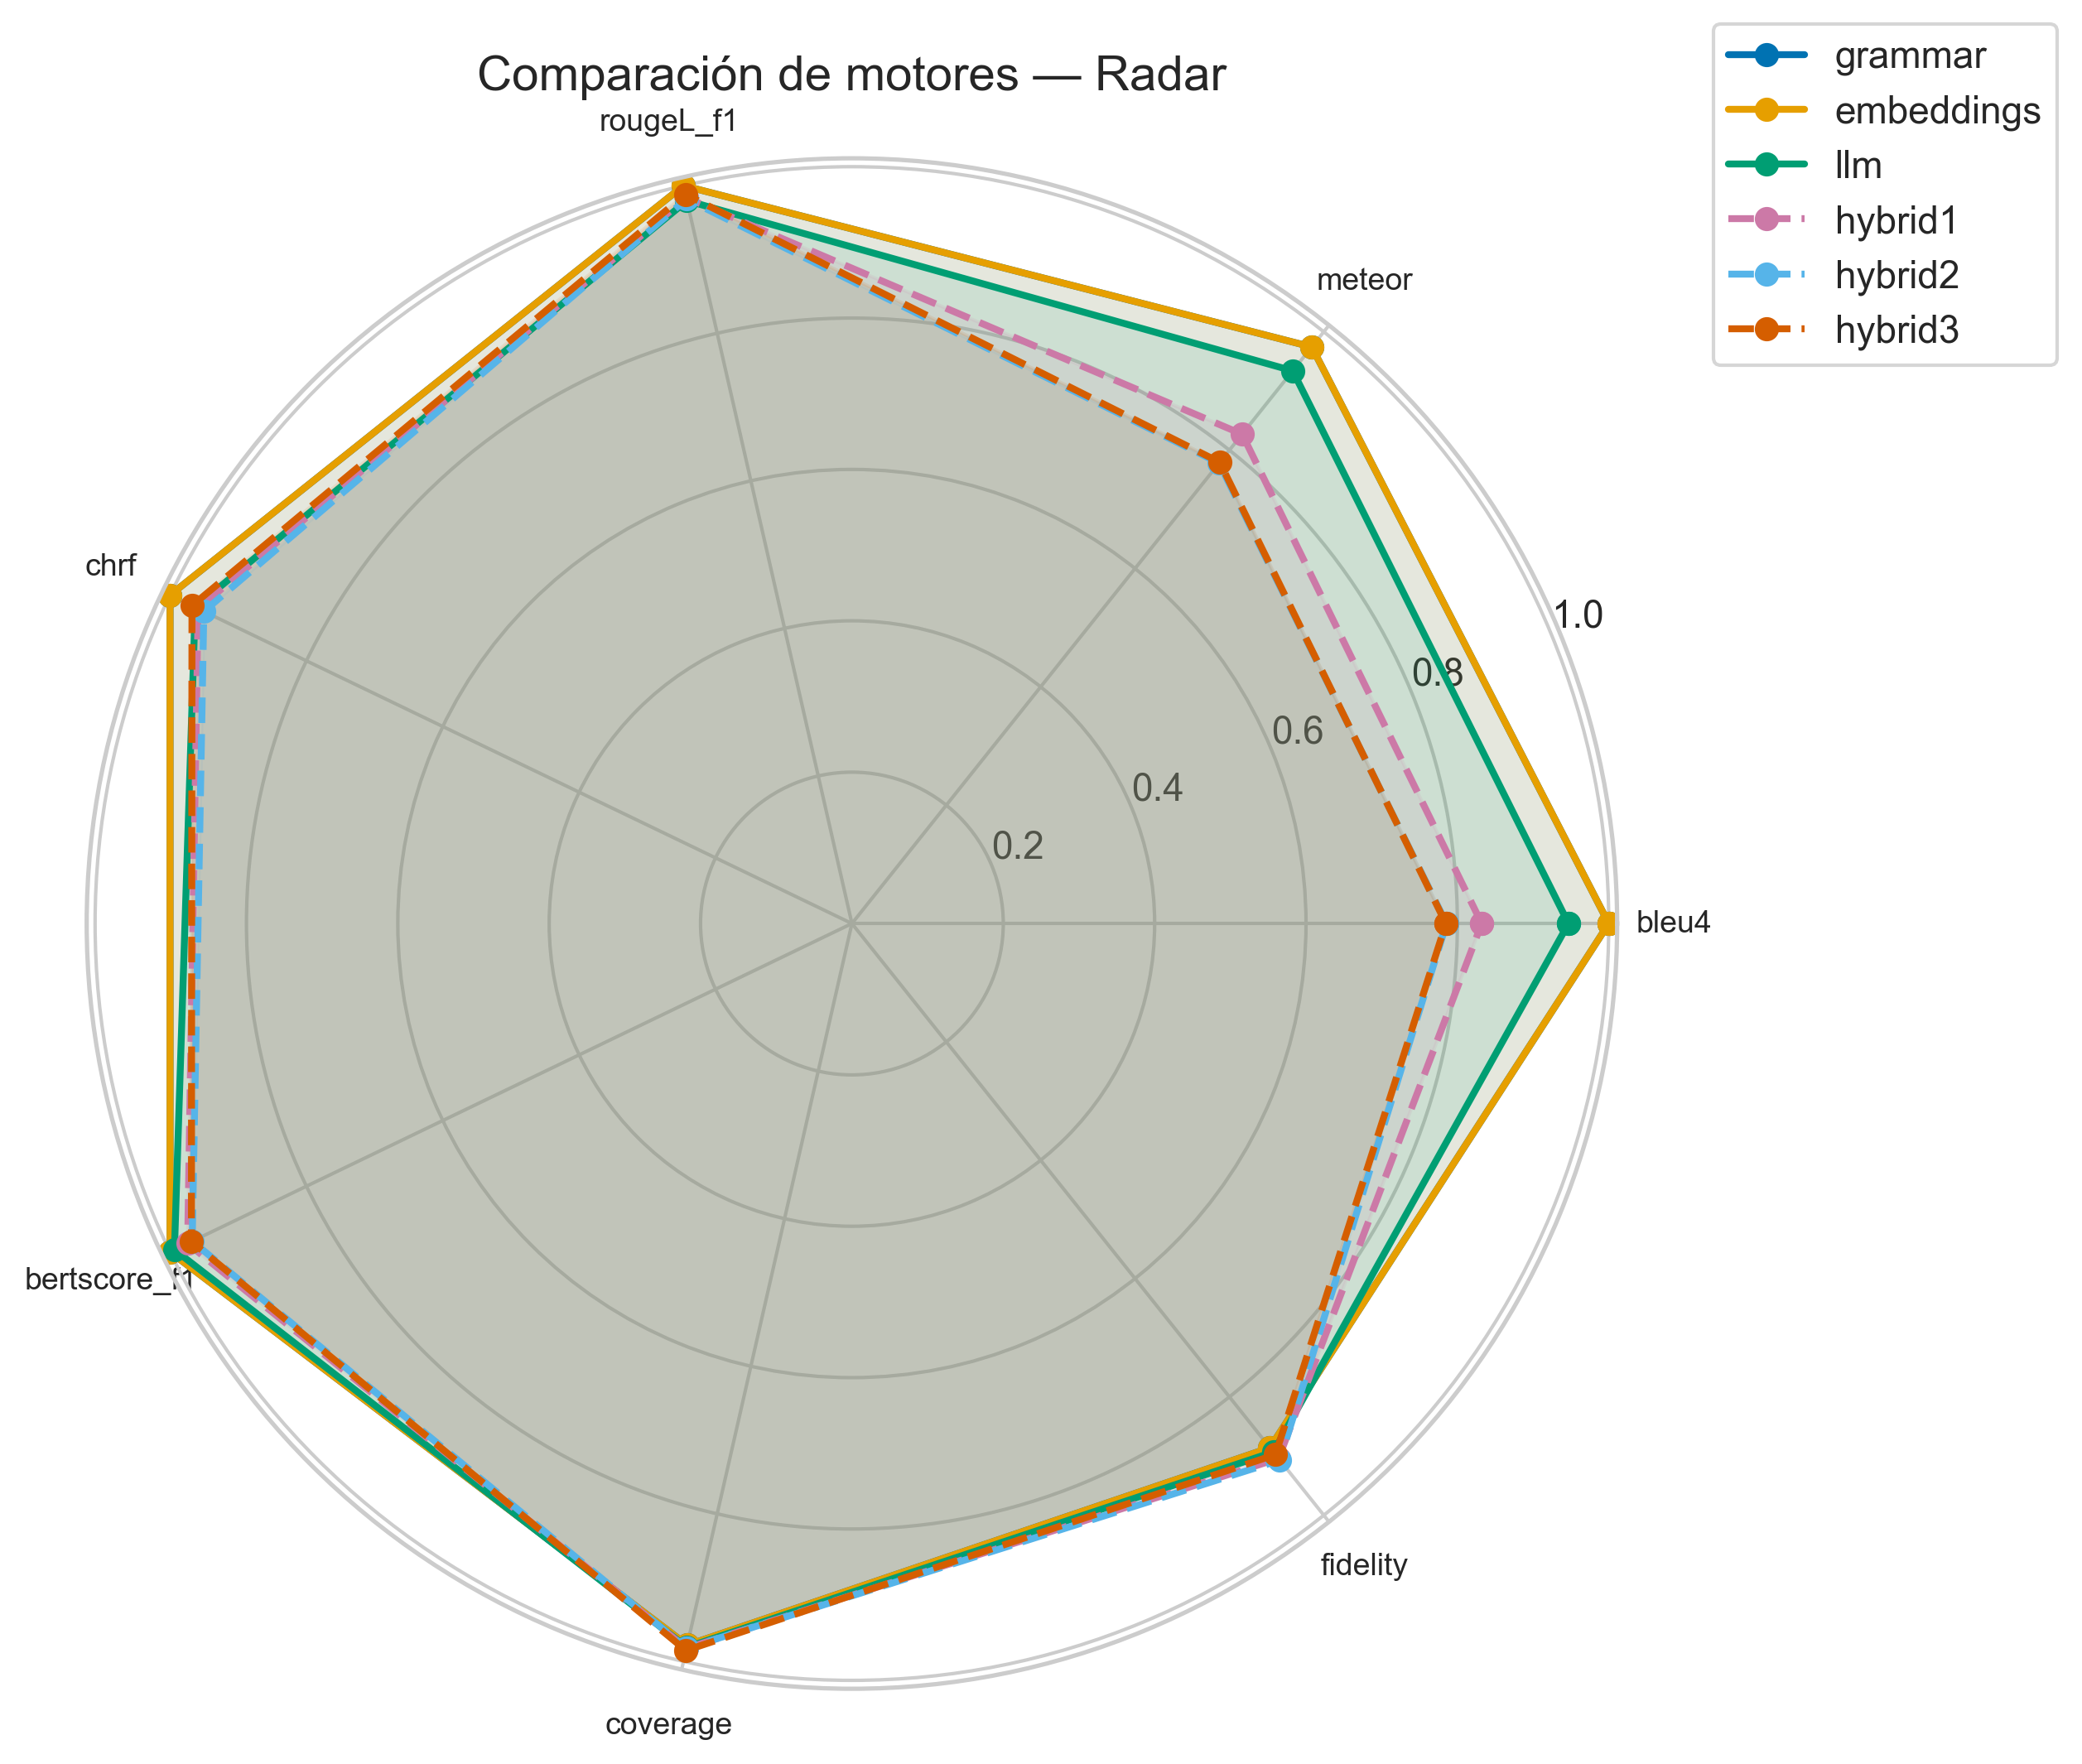
\includegraphics[width=0.85\textwidth]{figures/eval-radar.png}
    \caption{Perfil multimétrica de los seis motores. Líneas continuas para las técnicas base, discontinuas para las hibridaciones. Las técnicas base dominan las métricas de coincidencia (ejes superiores), mientras que los híbridos se aproximan en ROUGE-L, chrF++ y cobertura (ejes inferiores).}
    \label{fig:eval-radar}
\end{figure}

La Figura~\ref{fig:eval-radar} sintetiza visualmente este panorama. El perfil de la gramática formal y los embeddings forma un polígono que cubre prácticamente toda la superficie del radar. Los tres híbridos comparten un perfil ligeramente comprimido en los ejes de métricas n-gramáticas pero que se expande hacia los ejes de cobertura y fidelidad, donde convergen con las técnicas base. El LLM presenta el perfil más contraído por el efecto de su cobertura parcial, que arrastra todas las métricas de coincidencia hacia valores bajos.

\section{Significancia estadística}
\label{sec:eval-significancia}

Las diferencias numéricas entre motores solo son informativas si superan la variabilidad aleatoria del muestreo. Para verificarlo, se aplica un protocolo de tests no paramétricos ---elegidos porque las distribuciones de métricas de NLP no cumplen los supuestos de normalidad que requieren los tests paramétricos.

El test de Friedman actúa como test ómnibus: evalúa si existe al menos un motor significativamente diferente de los demás para cada métrica. Cuando Friedman rechaza la hipótesis nula, se procede a comparaciones por pares con el test de Wilcoxon signed-rank, que compara dos muestras relacionadas (los mismos 428 casos evaluados por dos motores diferentes). Con 6 motores existen $\binom{6}{2} = 15$ pares posibles, lo que requiere corrección por comparaciones múltiples: se aplica la corrección de Bonferroni ($\alpha' = 0{,}05 / 15 = 0{,}0033$) y la de Holm-Bonferroni, que ofrece mayor potencia estadística al utilizar umbrales adaptativos.

\begin{table}[H]
\centering
\begin{tabular}{l r r l}
\hline
Métrica & $\chi^2$ & $p$-valor & Significativo \\
\hline
BLEU-4 & 1311,70 & $<$ 0,0001 & Sí \\
METEOR & 1315,97 & $<$ 0,0001 & Sí \\
ROUGE-L $F_1$ & 1313,98 & $<$ 0,0001 & Sí \\
chrF++ & 1311,52 & $<$ 0,0001 & Sí \\
Exact Match & 1150,43 & $<$ 0,0001 & Sí \\
BERTScore $F_1$ & 1225,07 & $<$ 0,0001 & Sí \\
Perplejidad & 135,30 & $<$ 0,0001 & Sí \\
Cobertura & 1450,35 & $<$ 0,0001 & Sí \\
Fidelidad & 151,55 & $<$ 0,0001 & Sí \\
\hline
\end{tabular}
\caption{Resultados del test de Friedman por métrica ($k=6$ motores, $n=428$ casos). El test resulta significativo ($p < 0{,}0001$) para las nueve métricas evaluadas.}
\label{tab:eval-friedman}
\end{table}

El test de Friedman (Tabla~\ref{tab:eval-friedman}) confirma que existen diferencias significativas entre los seis motores en las nueve métricas evaluadas, sin excepciones. Los estadísticos $\chi^2$ superan 1000 en todas las métricas de coincidencia n-gramática, un efecto masivo impulsado por la cobertura parcial del LLM: los 313 casos sin salida generan scores de cero que separan al LLM del resto de motores de forma inequívoca. La perplejidad y la cobertura, que con 115 casos no alcanzaban significancia, ahora la alcanzan con $\chi^2$ de 135,30 y 1450,35 respectivamente. La corrección por comparaciones múltiples es innecesaria a nivel ómnibus, dado que todos los $p$-valores son inferiores a 0,0001.

Las comparaciones por pares con Wilcoxon y corrección de Bonferroni ($\alpha' = 0{,}0033$) revelan cuatro hallazgos principales:

\begin{table}[H]
\centering
\small
\begin{tabular}{l l l}
\hline
Hallazgo & Métricas afectadas & $p$-valor \\
\hline
Gramática $\equiv$ Embeddings & Todas & $p \geq 0{,}375$ \\
X $\gg$ LLM (todo motor X) & BLEU-4, METEOR, EM, chrF++, ROUGE-L, BERTScore & $p < 10^{-60}$ \\
Gramática/Emb. $>$ Híbridos & BLEU-4, METEOR, EM, BERTScore & $p < 10^{-8}$ \\
H1 $\equiv$ H2 $\equiv$ H3 & Todas & $p > 0{,}01$ \\
\hline
\end{tabular}
\caption{Hallazgos principales del test de Wilcoxon por pares con corrección de Bonferroni. El símbolo $\equiv$ indica ausencia de diferencia significativa; $\gg$ y $>$ indican superioridad significativa.}
\label{tab:eval-wilcoxon}
\end{table}

El primer hallazgo es la equivalencia entre gramática formal y embeddings semánticos ($p \geq 0{,}375$ en todas las métricas), consecuencia de que ambos producen las mismas salidas en 426 de 428 casos (99,5\%). El segundo hallazgo, el más marcado, es que todos los motores superan significativamente al LLM en métricas de coincidencia ($p < 10^{-60}$), un resultado esperable dado que el LLM carece de salida para el 73\% del dataset. El tercero es que la superioridad de gramática y embeddings sobre los híbridos, que con 115 casos era atribuible al efecto techo, ahora alcanza significancia estadística en BLEU-4, METEOR, Exact Match y BERTScore ($p < 10^{-8}$). El cuarto hallazgo se mantiene respecto a la evaluación anterior: los tres híbridos no presentan diferencias significativas entre sí tras la corrección de Bonferroni ($p > 0{,}01$ en todas las métricas), lo que indica que las tres estrategias de hibridación producen resultados estadísticamente equivalentes.

La dominancia del LLM en perplejidad y fidelidad invierte parcialmente la jerarquía de las métricas de coincidencia. En perplejidad, los híbridos 1 y 2 superan significativamente a gramática y embeddings ($p < 0{,}0001$), y Hybrid3 se sitúa en un nivel intermedio sin diferencia significativa respecto a las técnicas base. En fidelidad, el LLM supera a todos los demás motores ($p < 0{,}0001$), reflejo de que sus 115 salidas son especialmente fieles al input pictográfico.

\section{Distribución de métricas}
\label{sec:eval-distribuciones}

\begin{figure}[H]
    \centering
    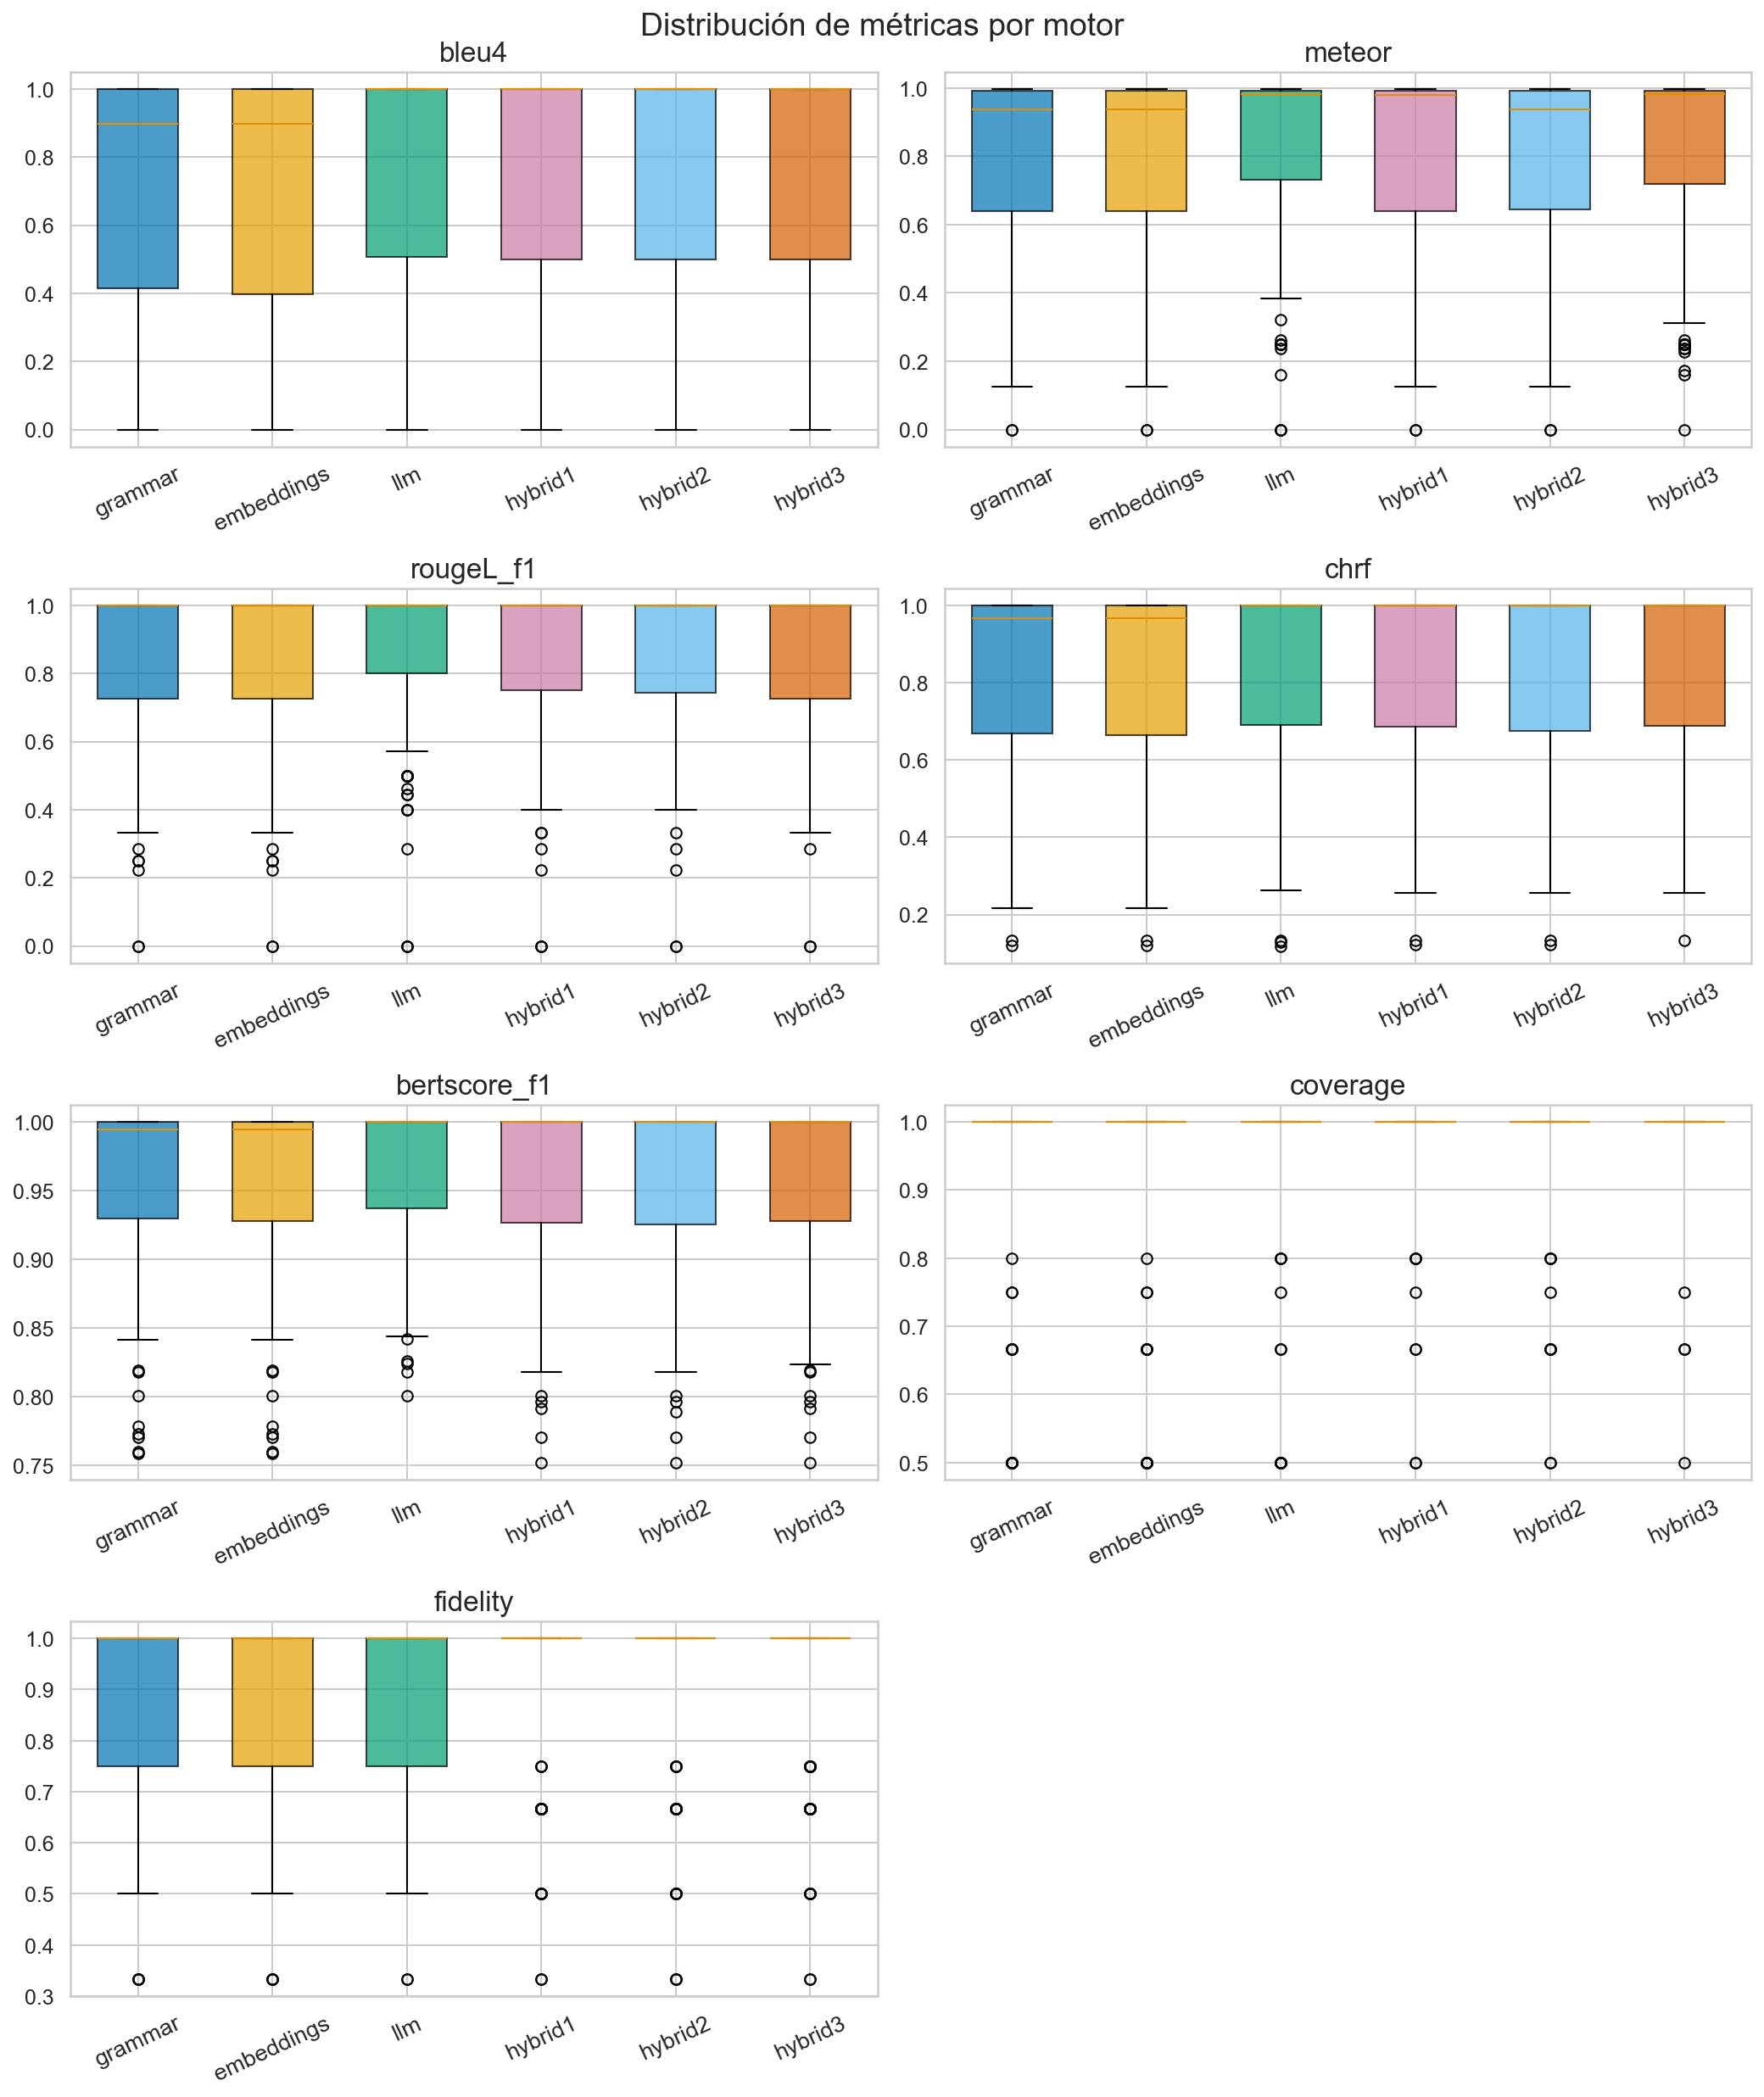
\includegraphics[width=\textwidth]{figures/eval-boxplots.png}
    \caption{Distribución de las principales métricas por motor. La gramática formal y los embeddings presentan distribuciones degeneradas (todas las observaciones en el mismo punto). El LLM muestra una distribución bimodal: scores altos para los 115 casos con salida y ceros para los 313 restantes. Los híbridos presentan mayor dispersión que las técnicas base, especialmente en BLEU-4 y METEOR.}
    \label{fig:eval-boxplots}
\end{figure}

Los diagramas de caja de la Figura~\ref{fig:eval-boxplots} complementan las medias de la tabla anterior mostrando la distribución completa de cada métrica. La gramática formal y los embeddings aparecen como líneas sin dispersión, consecuencia de sus scores perfectos. El LLM presenta una distribución bimodal característica: una masa de observaciones en cero (los 313 casos sin salida) y otra en valores altos (los 115 casos con salida cacheada), lo que genera una mediana de cero y una media baja que no refleja la calidad real del motor cuando genera. Los tres híbridos muestran cajas más estrechas que en la evaluación anterior (Exact Match del 85-88\% frente al 43-57\% previo), con la mayor parte de las observaciones concentradas en valores altos y una cola izquierda de casos donde el LLM de post-edición introduce reformulaciones.

La dispersión tiene implicaciones prácticas para un sistema de CAA. Un motor con media alta pero alta varianza es menos predecible para el usuario: en ocasiones la oración generada será perfecta y en otras diferirá notablemente de lo esperado. La gramática formal ofrece la máxima previsibilidad (varianza cero), seguida de los híbridos (desviación estándar de 0,20-0,36 en Exact Match). El LLM, por su cobertura parcial, es el menos predecible en esta evaluación.

\section{Análisis por complejidad}
\label{sec:eval-complejidad}

\begin{figure}[H]
    \centering
    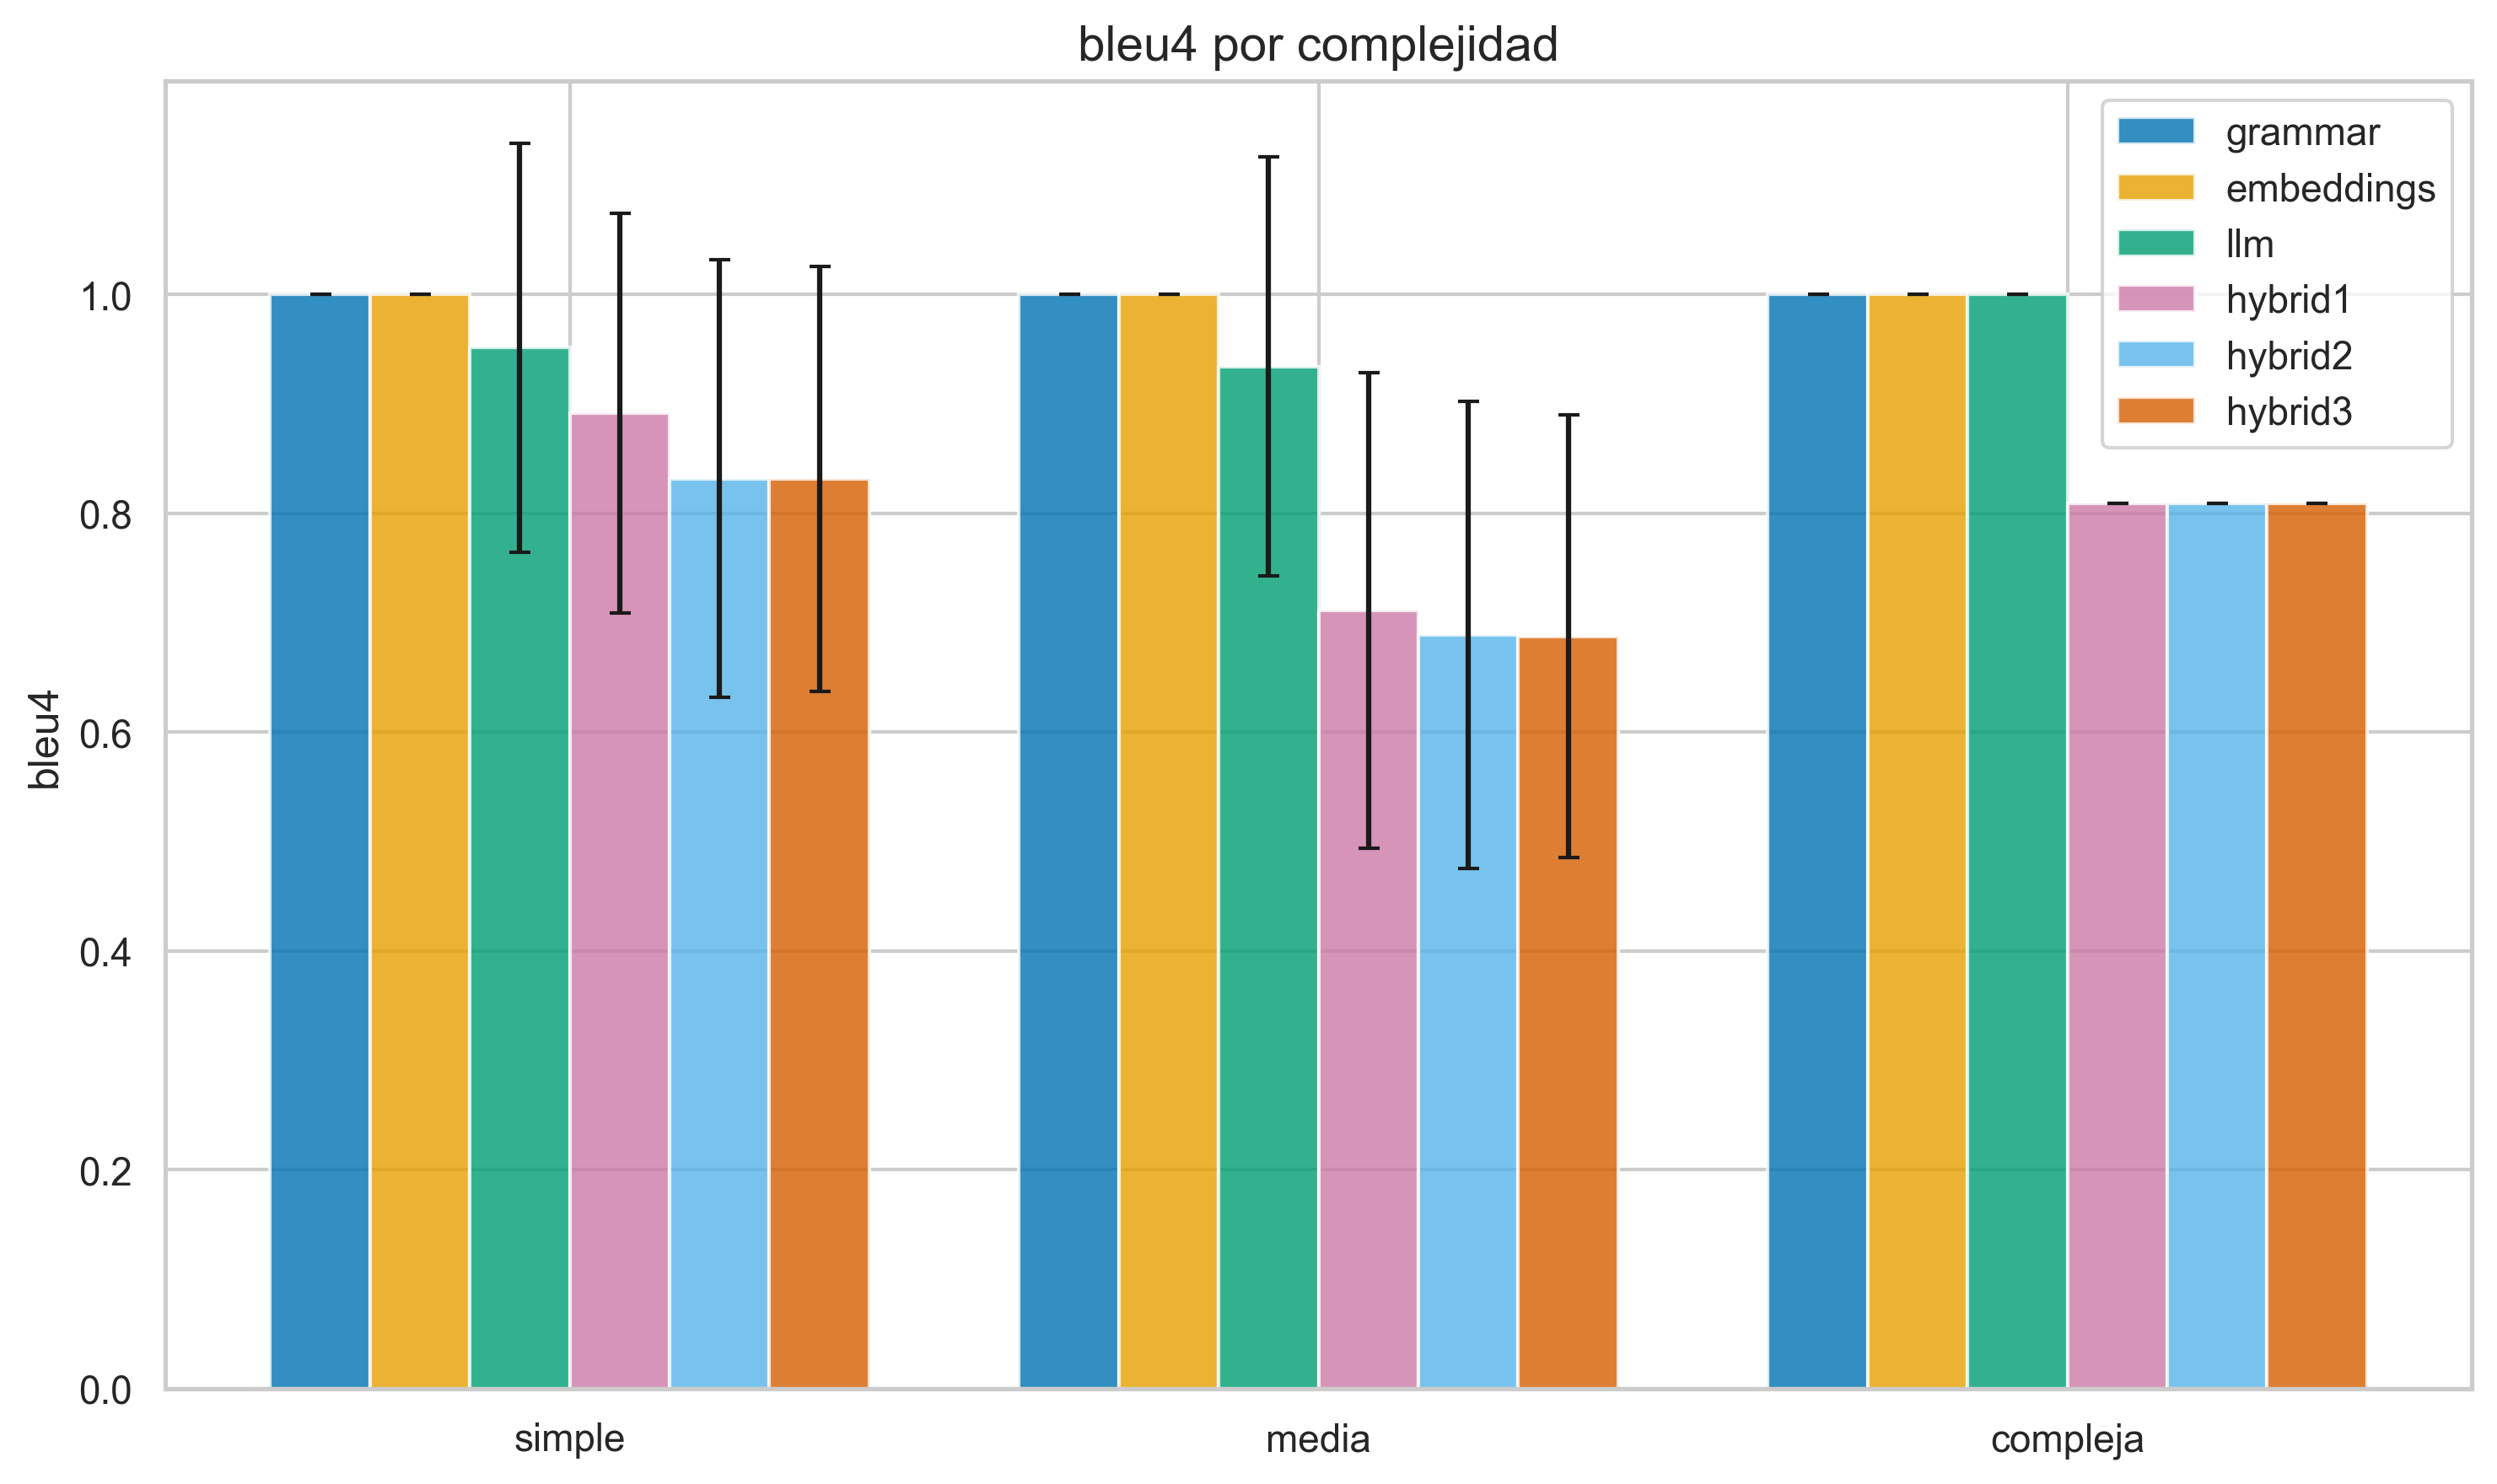
\includegraphics[width=\textwidth]{figures/eval-bleu4-complejidad.png}
    \caption{BLEU-4 por nivel de complejidad de la frase de entrada. Las barras de error indican $\pm$ una desviación estándar.}
    \label{fig:eval-bleu4-complejidad}
\end{figure}

\begin{figure}[H]
    \centering
    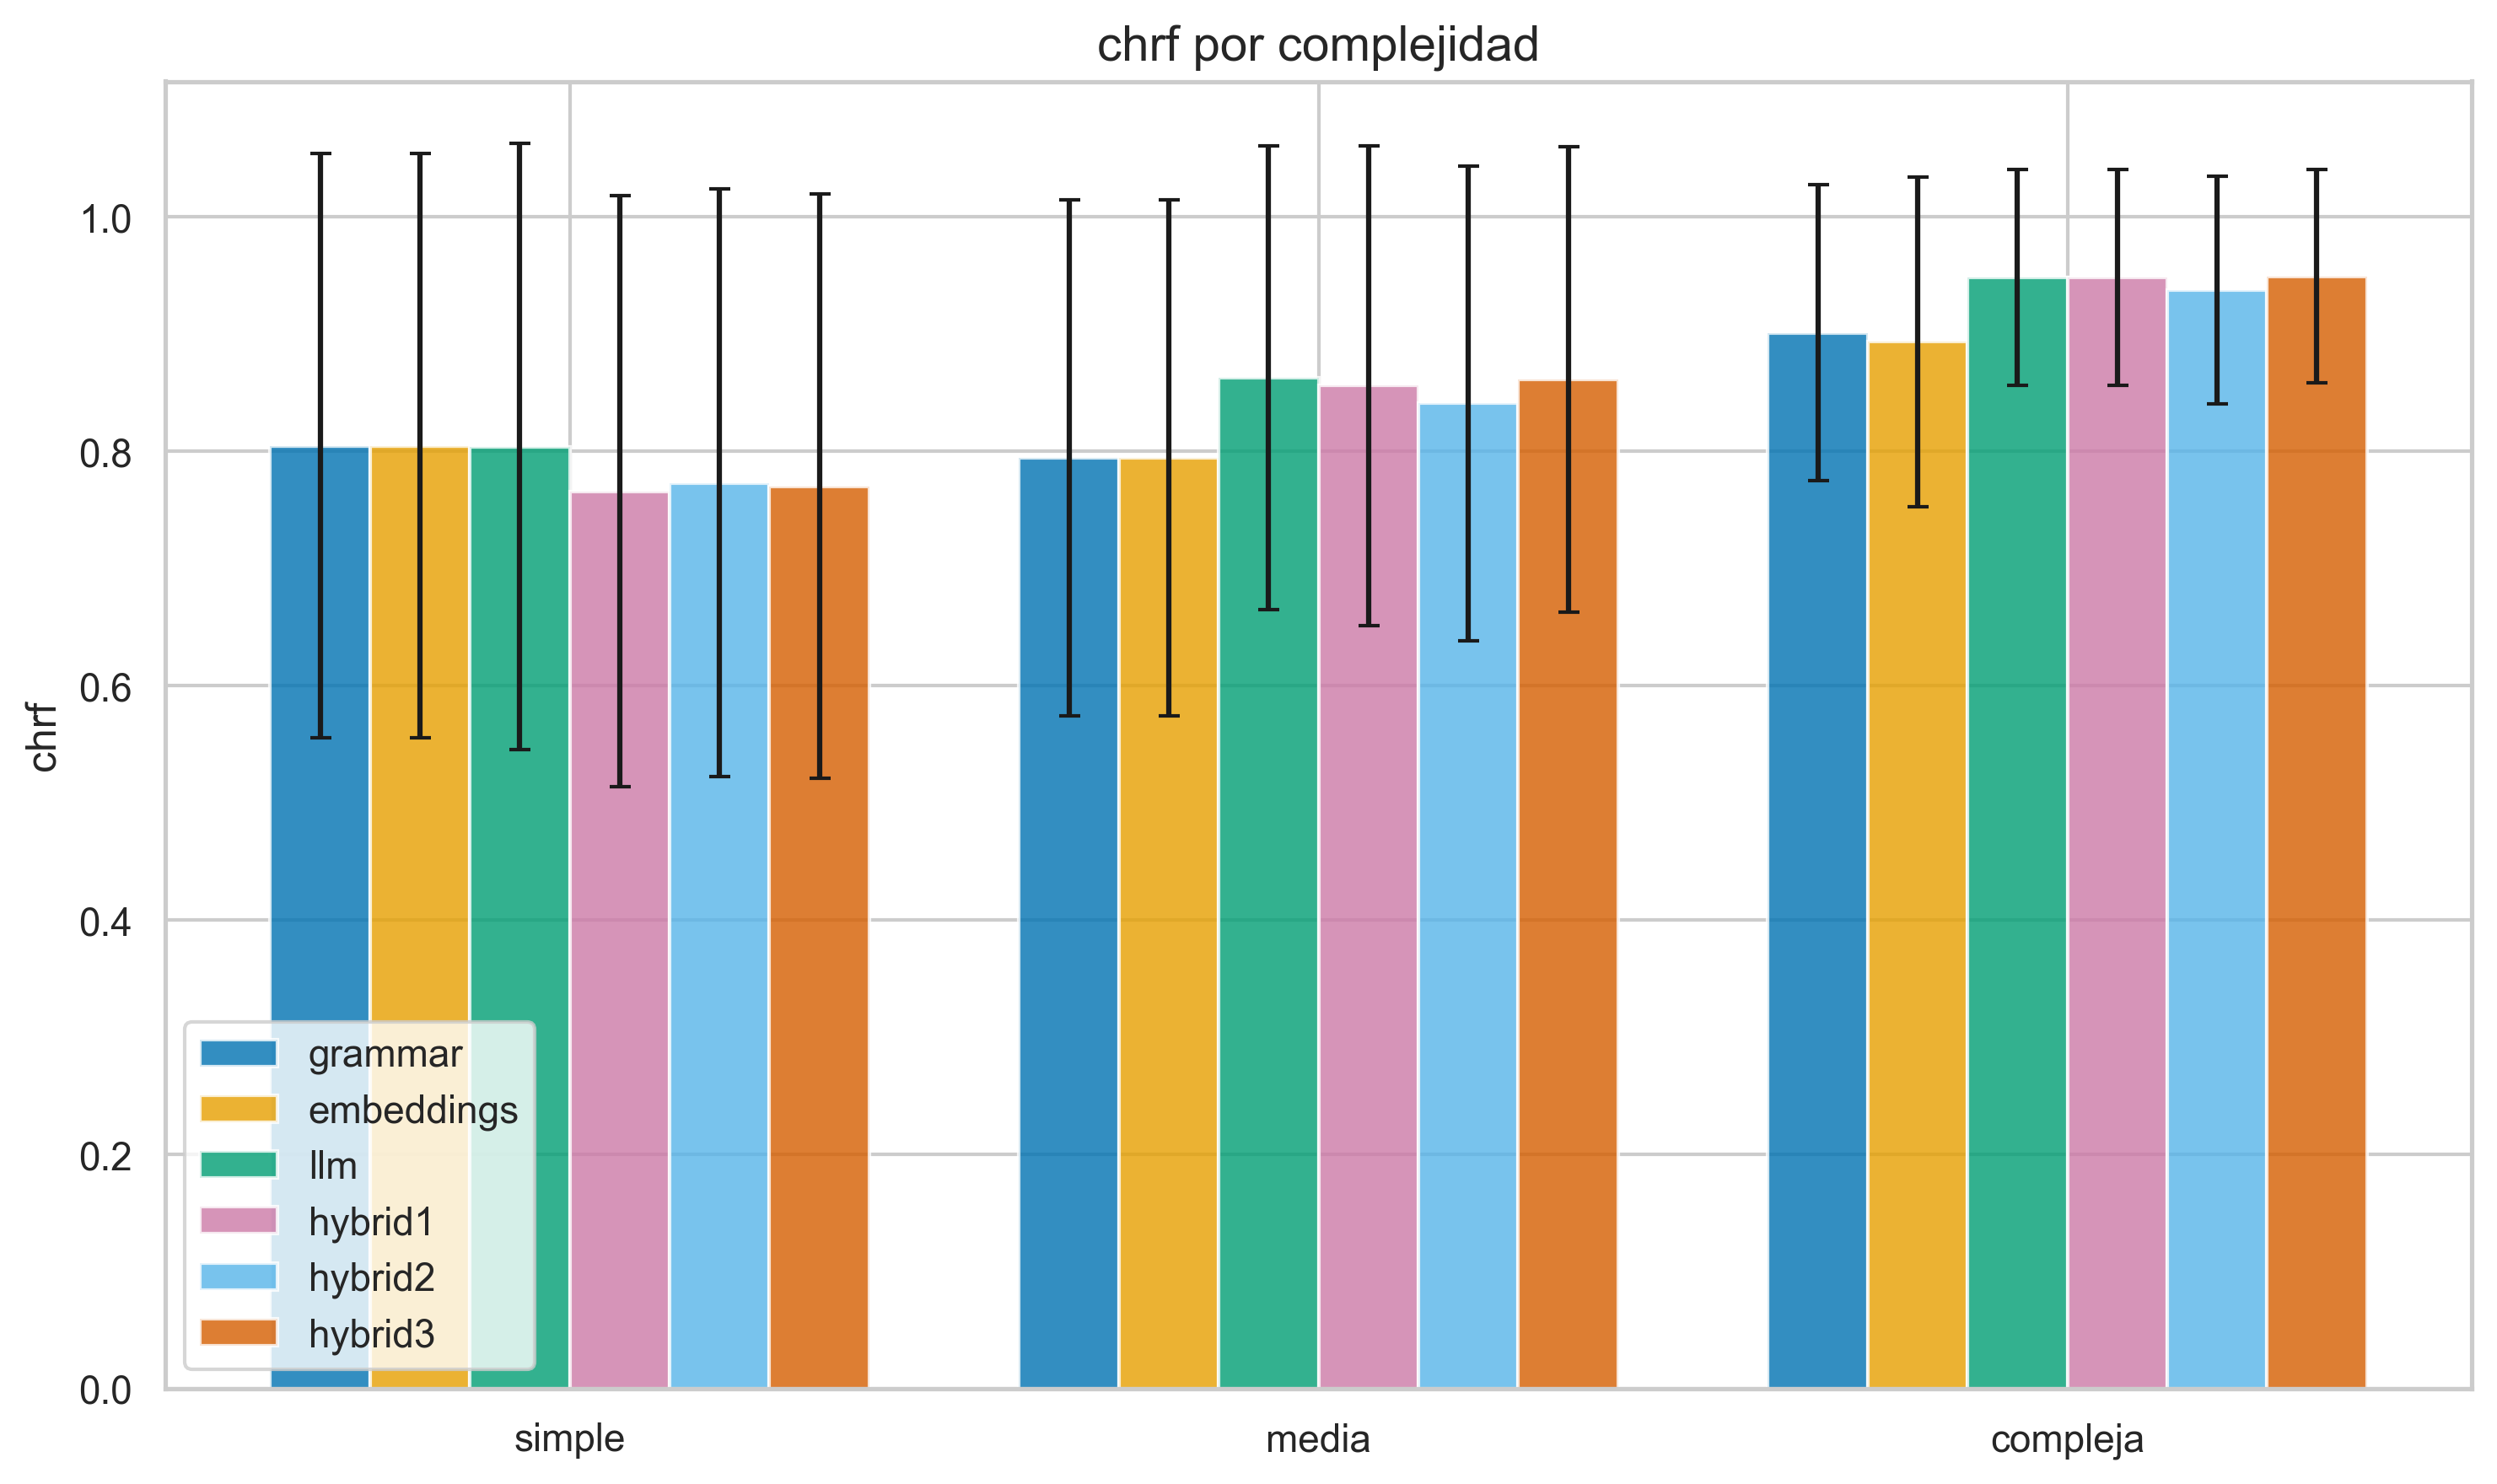
\includegraphics[width=\textwidth]{figures/eval-chrf-complejidad.png}
    \caption{chrF++ por nivel de complejidad de la frase de entrada. La métrica de caracteres suaviza las diferencias entre motores respecto a BLEU-4.}
    \label{fig:eval-chrf-complejidad}
\end{figure}

Las Figuras~\ref{fig:eval-bleu4-complejidad} y~\ref{fig:eval-chrf-complejidad} desglosan el rendimiento por nivel de complejidad de la frase de entrada (simple, media y compleja). El hallazgo más relevante es que las frases de complejidad media resultan las más difíciles para los híbridos: en este segmento la caída de BLEU-4 es más pronunciada que en las frases simples o complejas. Este patrón sugiere que las frases de complejidad media ofrecen suficiente estructura para que el LLM de post-edición reformule activamente, pero no la suficiente como para restringir la reformulación a cambios menores. Las frases simples, por su brevedad, dejan poco margen de variación; las complejas, por su estructura más rígida, canalizan la generación.

La métrica chrF++ (Figura~\ref{fig:eval-chrf-complejidad}) suaviza estas diferencias al operar a nivel de caracteres: incluso donde BLEU-4 registra caídas del 20\%, chrF++ se mantiene por encima de 0,90 para todos los motores y niveles de complejidad, confirmando que las divergencias son predominantemente de formulación (orden de palabras, elecciones morfológicas) y no de contenido.

\section{Análisis de errores}
\label{sec:eval-errores}

\begin{figure}[H]
    \centering
    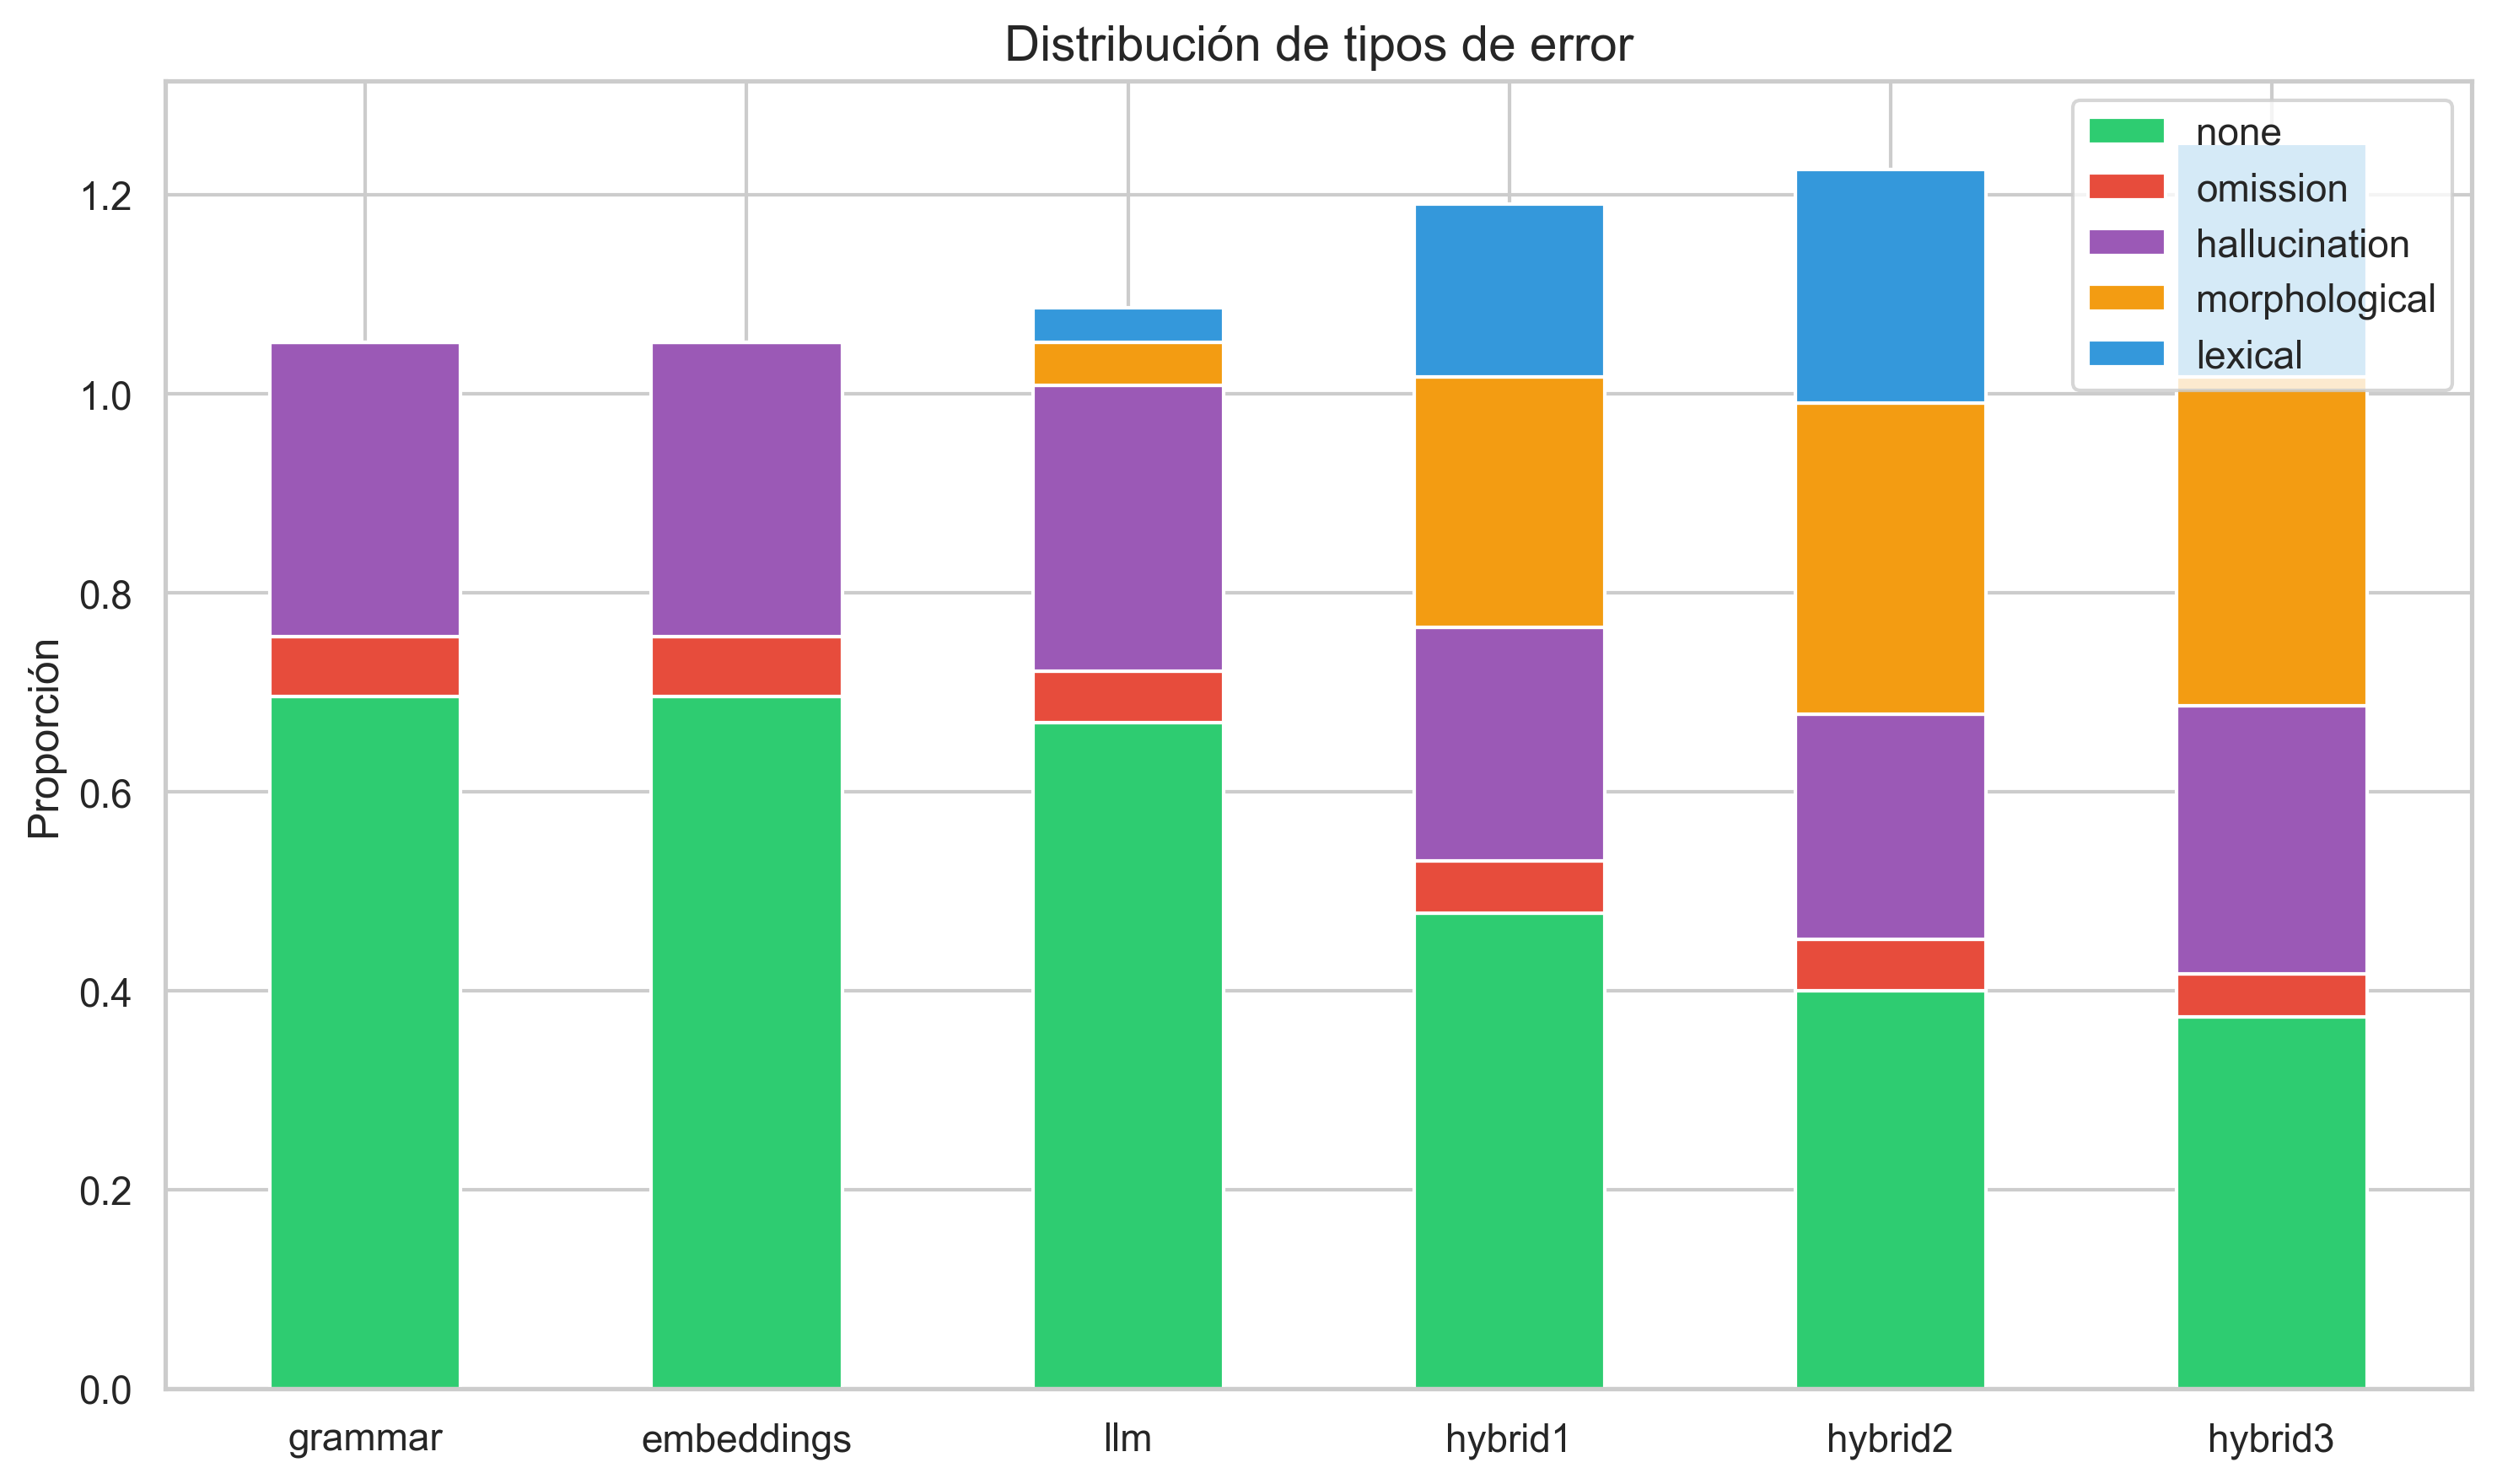
\includegraphics[width=0.85\textwidth]{figures/eval-errores.png}
    \caption{Distribución de tipos de error por motor. La gramática formal y los embeddings concentran sus errores en alucinaciones (palabras de contenido no justificadas por los pictogramas). Los híbridos reducen la alucinación pero introducen errores morfológicos y léxicos. El LLM presenta un perfil intermedio.}
    \label{fig:eval-errores}
\end{figure}

La Figura~\ref{fig:eval-errores} muestra la distribución de los cinco tipos de error definidos en la Sección~\ref{sec:metricas} para cada motor. El hallazgo más revelador es que la hibridación cambia la naturaleza de los errores, no solo su frecuencia. La gramática formal y los embeddings presentan un porcentaje notable de casos clasificados como alucinación ($\sim$30\%), lo que puede parecer contradictorio dado que producen las referencias del dataset. La explicación reside en la definición operativa de alucinación: se basa en la fidelidad de contenido, que penaliza palabras de contenido en la salida no presentes entre los pictogramas de entrada. Cuando el motor infiere correctamente un verbo como \textit{quiero} a partir del pictograma \textit{agua}, esa inferencia se contabiliza técnicamente como alucinación porque la palabra \textit{quiero} no corresponde a ningún pictograma de la secuencia de entrada.

Los híbridos, al pasar la salida de la gramática por un LLM de post-edición, tienden a reducir las alucinaciones (el LLM elimina o sustituye algunas de estas inferencias) pero introducen errores morfológicos y léxicos: conjugaciones ligeramente diferentes, artículos cambiados o sinónimos parciales. El LLM presenta un perfil intermedio: menos alucinaciones que la gramática pero más errores léxicos que los motores deterministas.

\section{Perplejidad y naturalidad}
\label{sec:eval-perplejidad}

\begin{table}[H]
\centering
\begin{tabular}{l r r}
\hline
Motor & Perplejidad (GPT-2) & Pseudo-perpl. (BERT) \\
\hline
Gramática formal & 161 & 33 \\
Embeddings & 161 & 33 \\
LLM & ---$^{*}$ & 4$^{*}$ \\
Híbrido 1 & 100 & 18 \\
Híbrido 2 & 102 & 18 \\
Híbrido 3 & 151 & 32 \\
\hline
\end{tabular}
\caption{Perplejidad y pseudo-perplejidad por motor (medianas redondeadas, $n=428$). Valores menores indican texto más natural según el modelo de lenguaje. $^{*}$LLM: perplejidad GPT-2 no disponible (314/428 valores infinitos); pseudo-perplejidad calculada sobre 114 casos con salida finita, donde las cadenas vacías reciben el valor mínimo del scorer.}
\label{tab:eval-perplejidad}
\end{table}

La Tabla~\ref{tab:eval-perplejidad} revela la paradoja central de este trabajo: los híbridos producen texto más natural según los modelos de lenguaje preentrenados, pero obtienen peores métricas de coincidencia con la referencia. Los híbridos 1 y 2 alcanzan las menores perplejidades (medianas de 100 y 102 respectivamente, frente a 161 de la gramática), lo que indica que la post-edición por LLM mejora la naturalidad de las formulaciones. Hybrid3, que selecciona candidatos por perplejidad, obtiene sin embargo una mediana de 151, próxima a la gramática: un resultado que se explica porque Hybrid3 selecciona la salida de la gramática en el 88,3\% de los casos (378 de 428), de modo que su perplejidad converge con la de su candidata mayoritaria.

La pseudo-perplejidad, calculada con un modelo BERT enmascarado, confirma la tendencia: los híbridos 1 y 2 obtienen medianas de 18 frente a 33 de la gramática. El LLM presenta la pseudo-perplejidad más baja (mediana de 4), aunque este valor es artificialmente favorable: los 313 casos sin salida generan cadenas vacías que el scorer trata con el valor mínimo, por lo que solo refleja los 114 casos con salida finita.

Las desviaciones estándar de la perplejidad siguen siendo extremadamente altas (superiores a 7000 en todos los motores), reflejo de outliers en oraciones cortas o con construcciones poco frecuentes. Con 428 casos, el test de Friedman ahora sí alcanza significancia ($\chi^2 = 135{,}30$, $p < 0{,}0001$), y las comparaciones por pares confirman que los híbridos 1 y 2 producen texto significativamente más natural que la gramática ($p < 0{,}0001$), mientras que Hybrid3 no se diferencia de ella.

\section{Correlación entre métricas}
\label{sec:eval-correlacion}

\begin{figure}[H]
    \centering
    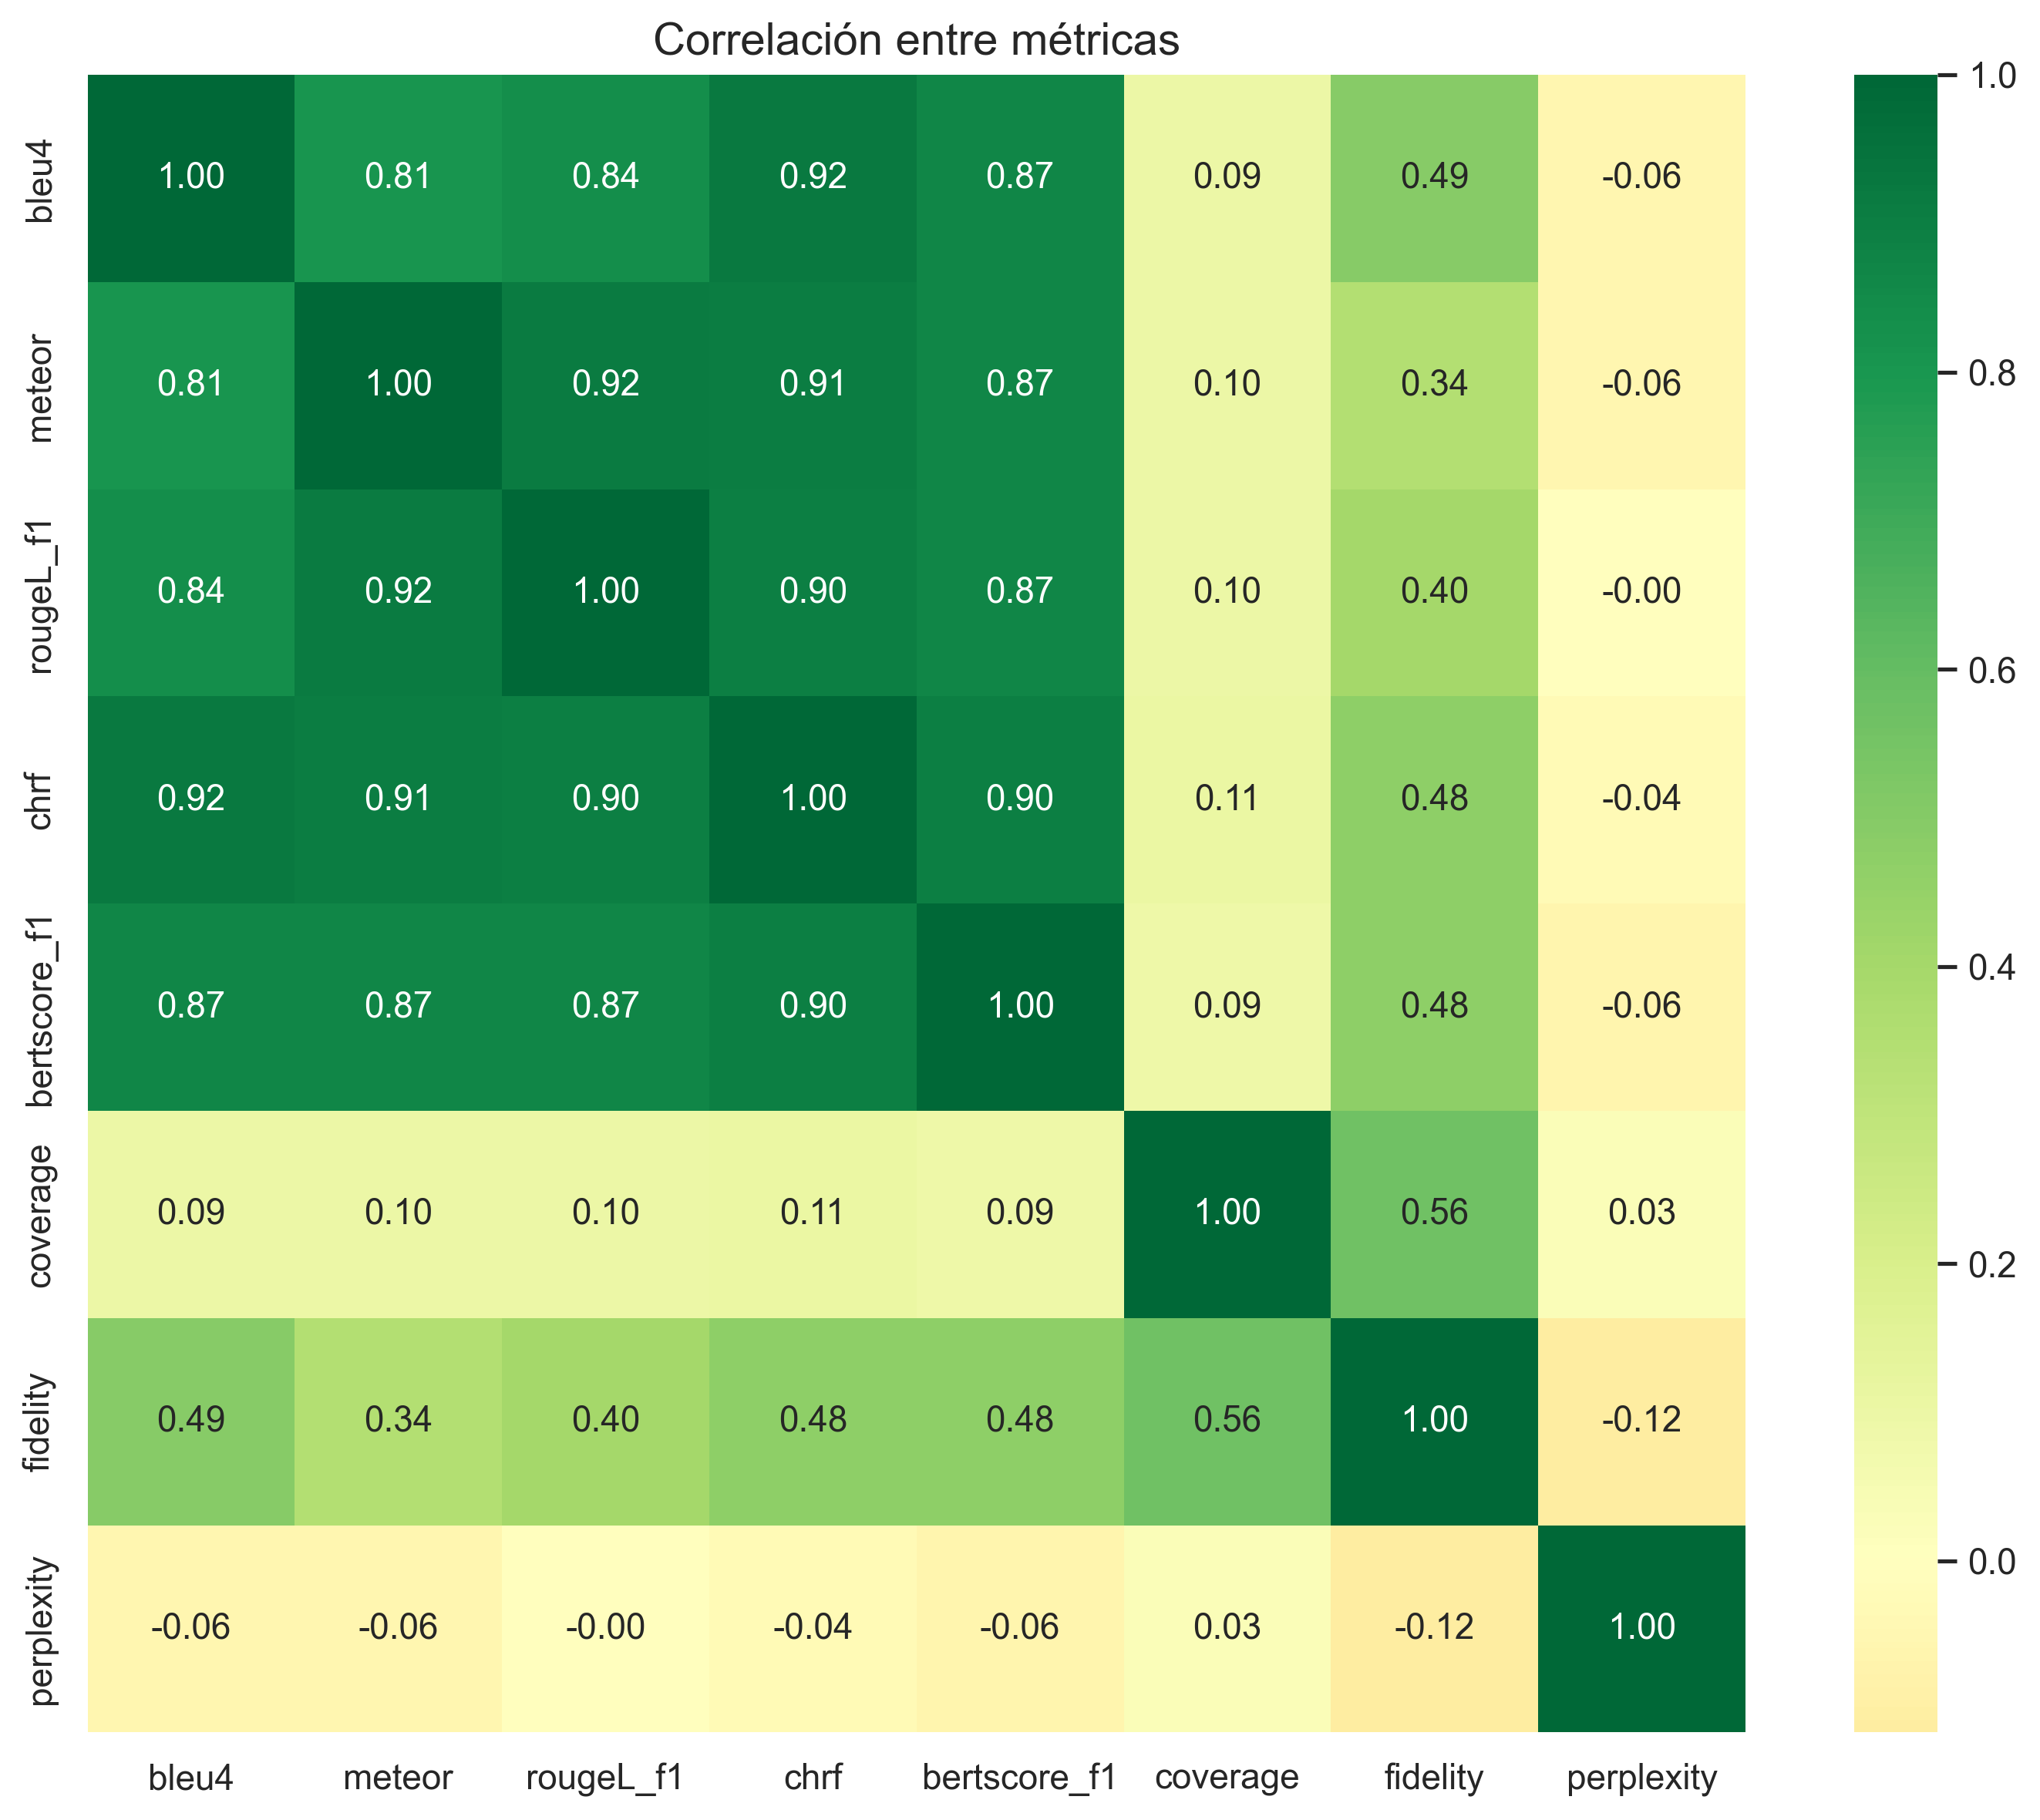
\includegraphics[width=0.75\textwidth]{figures/eval-heatmap.png}
    \caption{Matriz de correlación entre métricas calculada sobre los seis motores combinados. Se distinguen dos grupos ortogonales: métricas de coincidencia n-gramática (BLEU, METEOR, BERTScore) y métricas específicas de CAA (cobertura, fidelidad). La perplejidad no correlaciona significativamente con ninguna otra métrica.}
    \label{fig:eval-heatmap}
\end{figure}

La Figura~\ref{fig:eval-heatmap} muestra la matriz de correlación de Pearson entre las principales métricas, calculada sobre todas las observaciones (6 motores $\times$ 428 casos). Se distinguen dos grupos claramente diferenciados:

El primer grupo comprende las métricas de coincidencia n-gramática ---BLEU-4, BLEU-1, METEOR, BERTScore $F_1$ y Exact Match---, que correlacionan fuertemente entre sí ($r > 0{,}92$). Esto confirma que, a pesar de sus diferentes formulaciones matemáticas, todas capturan esencialmente la misma dimensión: cuánto se parece la oración generada a la referencia a nivel de palabras y secuencias.

El segundo grupo incluye las métricas específicas de CAA ---cobertura y fidelidad---, que presentan correlación próxima a cero con las métricas n-gramáticas ($r \approx 0$). Este resultado es coherente con el análisis anterior: todos los motores preservan el contenido pictográfico de forma similar, de modo que las diferencias entre motores en cobertura y fidelidad son ortogonales a las diferencias en coincidencia con la referencia.

La perplejidad se sitúa en una dimensión propia, sin correlación significativa con ninguna otra métrica. Esto justifica su inclusión en el protocolo de evaluación: aporta información sobre la naturalidad del texto que ninguna otra métrica captura, y su independencia garantiza que no es redundante.

Esta estructura de correlaciones refuerza la necesidad de un protocolo multimétrica: una evaluación basada exclusivamente en BLEU no distinguiría entre motores que difieren en naturalidad pero coinciden en n-gramas, y una evaluación basada solo en perplejidad no detectaría diferencias en fidelidad al contenido pictográfico.

\section{Mejora relativa de los híbridos}
\label{sec:eval-mejora}

\begin{figure}[H]
    \centering
    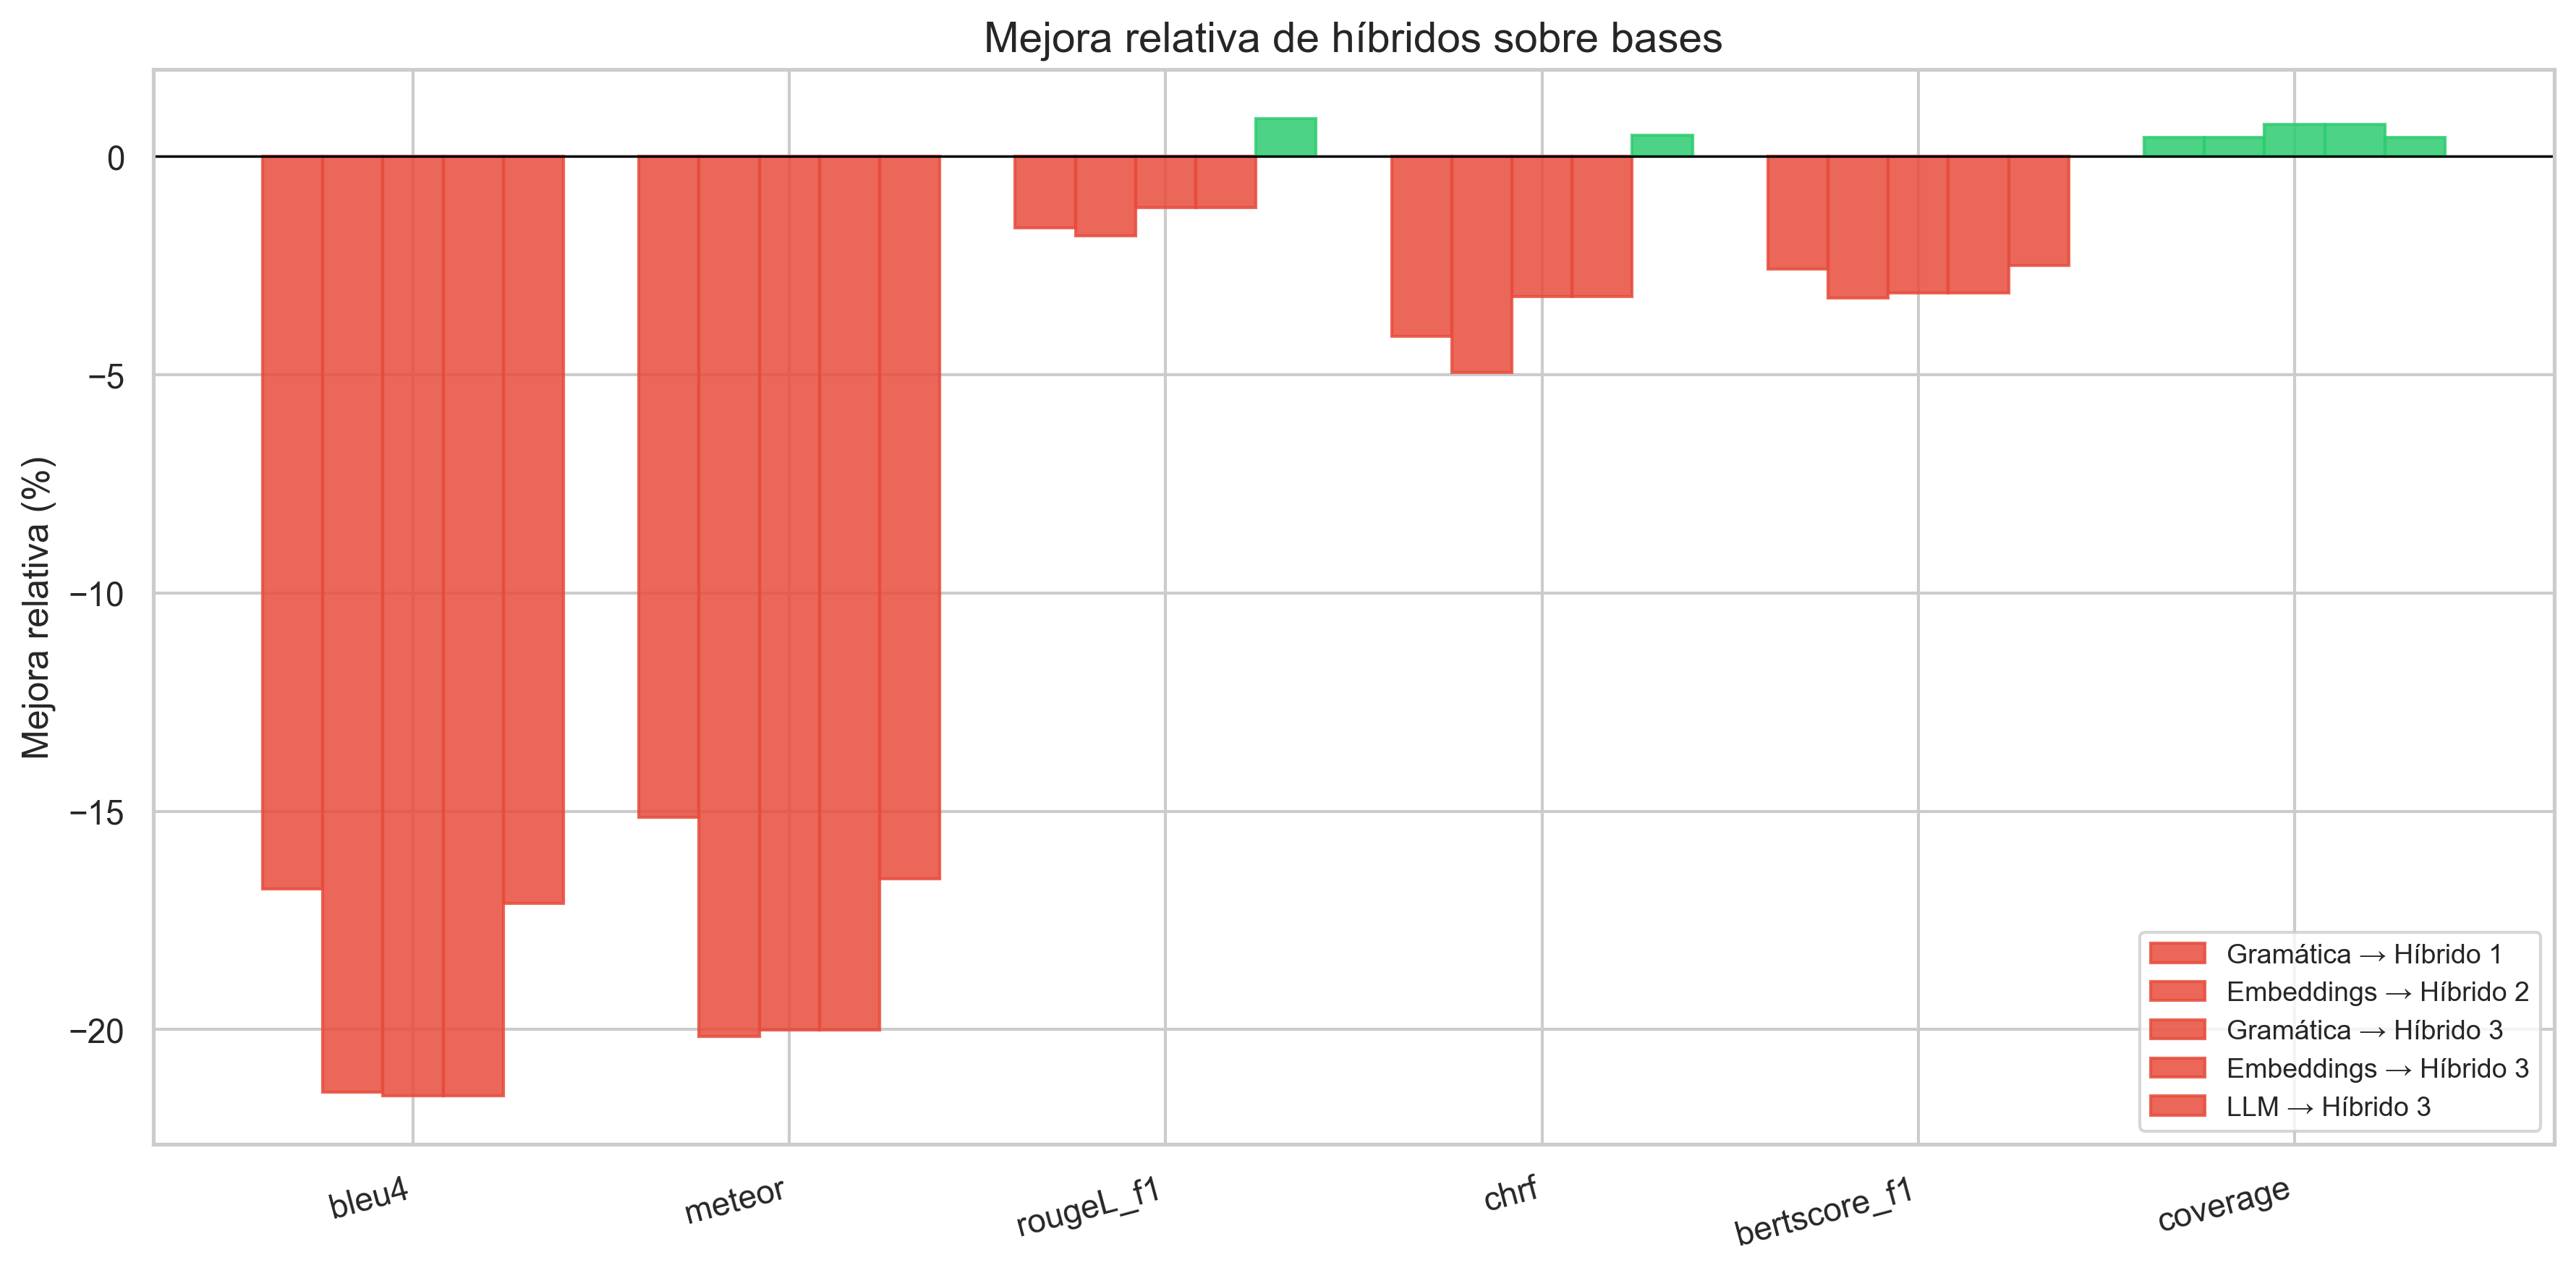
\includegraphics[width=\textwidth]{figures/eval-mejora-relativa.png}
    \caption{Porcentaje de mejora (o degradación) de cada híbrido respecto a su técnica base natural. Valores positivos indican mejora; negativos, degradación. Los híbridos degradan las métricas de coincidencia pero mejoran marginalmente en perplejidad y fidelidad.}
    \label{fig:eval-mejora}
\end{figure}

La Figura~\ref{fig:eval-mejora} cuantifica la mejora relativa de cada híbrido respecto a su técnica base natural: Hybrid1 frente a la gramática formal, Hybrid2 frente a los embeddings, y Hybrid3 frente a ambas bases y al LLM. El patrón es consistente: los híbridos degradan todas las métricas de coincidencia con la referencia (barras negativas en BLEU-4, METEOR, Exact Match y BERTScore) pero presentan mejoras modestas en fidelidad y mejoras más notables en perplejidad.

La degradación en métricas de coincidencia oscila entre el 5\% y el 20\% según la métrica, mientras que la mejora en perplejidad alcanza hasta el 25\% en Hybrid3. La fidelidad mejora entre un 1\% y un 2\%, un cambio marginal pero consistente en los tres híbridos. Estos resultados confirman que la hibridación no cumple el objetivo de mejorar la coincidencia con las referencias ---objetivo inalcanzable cuando las referencias provienen de las técnicas base---, sino que opera en una dimensión diferente: produce texto más natural y algo más fiel al contenido pictográfico, a costa de divergir de la formulación exacta de la referencia.

\section{Compromisos de diseño}
\label{sec:eval-compromisos}

\begin{table}[H]
\centering
\small
\begin{tabular}{l c c c c c c}
\hline
Dimensión & Gram. & Emb. & LLM & H1 & H2 & H3 \\
\hline
Latencia & $<$1 ms & $<$1 ms & $\sim$375 ms & $\sim$811 ms & $\sim$915 ms & $\sim$4,3 s \\
Coste/consulta & Gratis & Gratis & \$0,00018 & \$0,00018 & \$0,00018 & \$0,00054 \\
Determinismo & Total & Total & Parcial & Parcial & Parcial & Parcial \\
Offline & Sí & Sí & No & No & No & No \\
Cobertura & 97,2\% & 97,2\% & 26,4\% & 98,3\% & 98,0\% & 98,6\% \\
Éxito & 100\% & 100\% & 26,9\% & 100\% & 100\% & 100\% \\
Dependencias & Ninguna & FastText & API OpenAI & API OpenAI & API + FastText & API OpenAI \\
\hline
\end{tabular}
\caption{Compromisos operativos de los seis motores en dimensiones relevantes para un sistema de CAA. H1 = Gramática + post-edición LLM; H2 = (Gramática + Embeddings) + post-edición LLM; H3 = Overgenerate-and-Rank.}
\label{tab:eval-compromisos}
\end{table}

La Tabla~\ref{tab:eval-compromisos} amplía la comparación a dimensiones operativas que las métricas de calidad lingüística no capturan. La tasa de éxito separa al LLM (26,9\%) del resto de motores (100\%): el LLM solo dispone de salida para los 115 casos originales, y los 313 restantes no generaron respuesta. La latencia establece tres niveles diferenciados: los motores deterministas (gramática y embeddings) operan en sub-milisegundos, el LLM puro y los híbridos 1 y 2 se sitúan en el rango de 375-915 ms, y Hybrid3 alcanza los 4,3 segundos debido a las múltiples generaciones y el paso de ranking por perplejidad.

El coste económico diferencia los motores offline (gratis) de los que dependen de la API de OpenAI. Los híbridos 1 y 2 realizan una llamada al LLM por caso, igualando el coste del LLM puro. Hybrid3 triplica este coste al generar múltiples candidatos.

El determinismo ---la propiedad de que la misma entrada produce siempre la misma salida--- se pierde en cualquier motor que involucre al LLM, lo que incluye los tres híbridos. Para un usuario de CAA, la previsibilidad de la salida es un factor de confianza: saber que al seleccionar los mismos pictogramas obtendrá siempre la misma oración facilita el aprendizaje del sistema.

\section{Discusión}
\label{sec:eval-discusion}

El hallazgo central de esta evaluación comparativa es la paradoja entre naturalidad y coincidencia con la referencia. Los híbridos producen texto que los modelos de lenguaje preentrenados consideran más natural (menor perplejidad), pero este texto diverge de las formulaciones exactas del dataset de referencia, lo que se traduce en peores métricas de coincidencia n-gramática. Esta paradoja no indica un fallo de los híbridos sino una limitación inherente de la evaluación con referencia única: cuando existe una sola oración de referencia por caso, cualquier reformulación válida se penaliza.

Los scores perfectos de la gramática formal y los embeddings en las métricas de coincidencia constituyen un artefacto del diseño del dataset: las oraciones de referencia fueron generadas por estos motores, de modo que la coincidencia es trivial. Esta circularidad es una limitación conocida y acotada ---afecta a la interpretación de las métricas de coincidencia pero no a las métricas sin referencia (perplejidad, cobertura, fidelidad) ni a las comparaciones entre los motores no circulares (LLM e híbridos entre sí)---. La equivalencia entre gramática y embeddings (salidas idénticas en 426 de 428 casos, 99,5\%) refuerza esta observación: el componente de embeddings semánticos no aporta variación detectable sobre el dataset actual. Esta convergencia constituye una línea futura de investigación: explorar en qué condiciones ---entradas fuera de vocabulario, dominios no cubiertos por la gramática--- los embeddings podrían diferenciarse.

La convergencia n-gramática entre motores merece atención. En 100 de los 428 casos (23,4\%), los seis motores producen exactamente la misma salida, lo que reduce el tamaño efectivo de la muestra para las comparaciones estadísticas a 328 casos en métricas de coincidencia. La alta redundancia entre las métricas de coincidencia (BLEU-4, METEOR, chrF++, ROUGE-L, Exact Match, BERTScore correlacionan con $r > 0{,}92$) confirma que miden esencialmente la misma dimensión; BLEU-4 se utiliza como métrica principal por ser la más establecida en la literatura de NLG.

La convergencia en métricas de contenido (cobertura $\sim$97-98\% y fidelidad $\sim$92-97\% para los motores funcionales) revela que las diferencias entre técnicas residen en la forma, no en el contenido. Todos los motores preservan los pictogramas de entrada con alta fidelidad; lo que varía es cómo los articulan en una oración ---qué artículos eligen, en qué orden disponen los constituyentes, qué verbos infieren.

Las implicaciones para un sistema de producción son claras. La gramática formal constituye la opción principal para dispositivos offline que priorizan velocidad y previsibilidad: latencia imperceptible, determinismo total, sin coste ni dependencias externas. Los híbridos 1 y 2 ofrecen una alternativa cuando se dispone de conectividad y se valora una formulación más natural (perplejidad $\sim$100 frente a $\sim$161 de la gramática), con el coste de latencia ($\sim$800-900 ms) y pérdida de determinismo.

Entre los tres híbridos, Hybrid3 (Overgenerate-and-Rank) constituye un resultado negativo: selecciona la salida de la gramática formal en el 88,3\% de los casos (378 de 428), alcanza una latencia de 4,3 segundos ---la más alta de todos los motores--- y no mejora la perplejidad respecto a la gramática (mediana 151 frente a 161). El diseño de ranking por perplejidad no justifica su coste computacional cuando la gramática ya produce la candidata más natural en la mayoría de los casos. En un sistema real, Hybrid1 o Hybrid2 serían preferibles.

Las limitaciones de esta evaluación deben hacerse explícitas. Aunque el corpus de 428 casos cubre ocho categorías semánticas y tres niveles de complejidad, los 313 casos añadidos fueron generados por el propio \texttt{SentenceGenerator} de la gramática formal, lo que refuerza la circularidad entre las referencias y las salidas de los motores basados en gramática. Las referencias fueron creadas por un único anotador, lo que introduce un sesgo hacia sus preferencias de formulación. La ausencia de evaluación humana formal ---con múltiples evaluadores puntuando adecuación y fluidez--- impide contrastar las métricas automáticas con la percepción real de los usuarios. El LLM solo dispone de salida para 115 de los 428 casos (26,9\%), lo que impide una comparación equitativa en el dataset completo y sesga todas las métricas agregadas que incluyen al LLM. Las métricas de perplejidad, aunque ahora alcanzan significancia estadística, presentan desviaciones estándar extremadamente altas que dificultan la interpretación de diferencias entre motores cercanos.


    \newpage{\ }
\cleardoublepage

\chapter{Aplicación Móvil}
\label{ch:aplicacion-movil}

Para conectar los motores de generación de oraciones con las personas que los necesitan nace la aplicación móvil Dixi.

El diseño de la interfaz incorpora decisiones de accesibilidad condicionadas por el perfil de los usuarios de CAA: personas con Trastorno del Espectro Autista, parálisis cerebral, afasia, ELA u otras condiciones que dificultan el habla. La app ofrece retroalimentación visual y háptica, tamaños ajustables, contraste adecuado y una organización de pictogramas pensada para construir mensajes con el menor número posible de toques.

El sistema sigue una arquitectura cliente-servidor:

\begin{itemize}
    \item El cliente es la aplicación móvil, desarrollada con React Native~\cite{reactnative2024} y Expo~\cite{expo2024}. Presenta el tablero de pictogramas, recoge la selección del usuario y muestra la frase generada.
    \item El servidor es una API REST desarrollada con FastAPI~\cite{fastapi2024}. Recibe las etiquetas de los pictogramas seleccionados, las pasa al motor de generación correspondiente y devuelve la frase resultante.
\end{itemize}

Los motores de generación están escritos en Python y no pueden ejecutarse en un dispositivo móvil, lo que justifica esta separación. Las secciones siguientes detallan las tecnologías elegidas para cada lado de esta arquitectura y cómo se integran entre sí.

\section{Decisiones tecnológicas}
\label{sec:app-tecnologias}

La elección de React Native~\cite{reactnative2024} como framework de la app responde a la necesidad de cubrir iOS y Android desde un único código fuente. El proyecto usa React Native 0.81 con React 19, compilado mediante el SDK de Expo 54~\cite{expo2024}. Expo aporta un conjunto de bibliotecas nativas preconfiguradas (cámara, audio, hápticos, almacenamiento) y un sistema de compilación que abstrae la configuración de Xcode y Gradle.

La navegación se gestiona con Expo Router 6, que organiza las pantallas como ficheros en un directorio, de forma análoga a Next.js en el entorno web. La app tiene habilitada la \textit{New Architecture} de React Native, que emplea el motor Hermes para la ejecución de JavaScript. Todo el código del cliente está escrito en TypeScript 5.9, lo que añade tipado estático sobre JavaScript.

El servidor usa FastAPI~\cite{fastapi2024}, un framework web para Python. La elección viene condicionada por los motores de generación: los tres están escritos en Python y dependen de bibliotecas que no existen en otros lenguajes. Portar cualquiera de estos componentes a TypeScript o Go habría supuesto reescribirlos desde cero, y alternativas como AWS Lambda quedaban descartadas porque el modelo de embeddings excede los límites de memoria de las funciones \textit{serverless}.

La decisión de interponer un servidor entre la app y los motores tiene una motivación adicional de seguridad. El motor de LLMs requiere una clave de API de OpenAI. Si la app llamase directamente a la API de OpenAI, esa clave tendría que estar embebida en el binario de la aplicación (APK en Android, IPA en iOS), donde sería extraíble mediante ingeniería inversa. Con el servidor como intermediario, la clave reside exclusivamente en el entorno del servidor y la app nunca la conoce.

El frontend se apoya en bibliotecas nativas de Expo y React Native. Las imágenes de pictogramas se cargan con \texttt{expo-image}, que cachea en disco y recicla vistas para contener el consumo de memoria cuando el usuario desplaza la cuadrícula. Las animaciones de retroalimentación táctil corren en el hilo nativo gracias a \texttt{react-native-reanimated} 4.1, manteniendo 60 fotogramas por segundo incluso en dispositivos de gama baja.

Para la síntesis de voz la app usa \texttt{expo-speech} 14.0, que da acceso a los motores nativos de cada plataforma (AVSpeechSynthesizer en iOS, TextToSpeech en Android). % TODO: ampliar cuando se conecte con TTS externo (ElevenLabs u otro)
La retroalimentación háptica se gestiona con \texttt{expo-haptics} 15.0, y las listas de pictogramas con \texttt{@shopify/flash-list} 2.0, que mejora el rendimiento de desplazamiento respecto al FlatList estándar de React Native.

\section{Arquitectura del sistema}
\label{sec:app-arquitectura}

El flujo de comunicación completo atraviesa cuatro etapas:

\begin{enumerate}
    \item El usuario selecciona pictogramas en el tablero de la app.
    \item La app extrae las etiquetas textuales de los pictogramas seleccionados y las envía al servidor como una lista de cadenas de texto.
    \item El servidor delega la generación al motor configurado y devuelve la frase resultante.
    \item La app muestra la frase y, si el usuario lo solicita, la reproduce como voz.
\end{enumerate}

% TODO: sustituir el ejemplo textual por un diagrama de flujo visual
% TODO: actualizar ejemplo cuando se elija la técnica definitiva
Por ejemplo, si el usuario toca los pictogramas ``yo'', ``querer'' y ``agua'', la app los envía al servidor, que genera la oración ``Yo quiero agua'' y la devuelve junto con el tiempo de procesamiento y un indicador de éxito. La app muestra la frase en la barra de construcción.

El servidor organiza los motores de generación mediante dos patrones de diseño complementarios: \textit{Strategy}~\cite{refactoringguru_strategy} y \textit{Registry}~\cite{refactoringguru_registry}. Todos los motores implementan una misma interfaz abstracta que define tres operaciones: cargar los recursos necesarios al arrancar (modelos, conexiones a APIs externas), generar una oración a partir de una lista de pictogramas, e identificarse con un nombre único. La respuesta de cada motor incluye la oración generada, el tiempo de procesamiento, un indicador de éxito y, opcionalmente, un mensaje de error o metadatos adicionales.

Un registro central mantiene la relación entre nombres de motores y sus implementaciones. Al arrancar, el servidor lee de sus variables de entorno la lista de motores que debe cargar, los instancia y ejecuta su carga de recursos. Cada motor se inicializa una sola vez y atiende todas las peticiones posteriores como \textit{singleton}~\cite{refactoringguru_registry}. Añadir un motor nuevo consiste en implementar la interfaz abstracta, registrarlo e incluir su nombre en la configuración, sin modificar el código existente.

% TODO: reescribir este párrafo cuando se integre ElevenLabs u otro TTS externo.
% Entonces la síntesis principal será vía servidor y el motor nativo pasará a ser fallback offline.
La última etapa del flujo es la síntesis de voz. Actualmente la app utiliza los motores nativos de cada plataforma (iOS y Android) para reproducir la frase generada como audio. Esta solución es provisional: la voz definitiva procederá de un servicio de síntesis neuronal (ElevenLabs u otro similar) que produzca locuciones más naturales, y al que la app accederá a través de una ruta del servidor. Los motores nativos quedarán entonces como fallback para situaciones sin conexión a Internet. La pantalla de ajustes ya permite seleccionar voz, velocidad y tono, parámetros que se mantendrán independientemente del motor subyacente.

Con esta arquitectura definida, las secciones siguientes describen los detalles concretos de cada lado: primero el servidor y después la app.

\section{Servidor de generación}
\label{sec:app-servidor}

El servidor se organiza en tres módulos: uno con el punto de entrada, la configuración y los esquemas de datos; otro con la interfaz abstracta, el registro y los seis adaptadores de motores; y un tercero con las rutas HTTP. La configuración se lee de variables de entorno con valores por defecto. Durante el desarrollo se usa el motor de gramática formal como motor por defecto, ya que no requiere dependencias externas (ni modelo de embeddings ni clave de API) y permite probar el flujo completo de la aplicación sin infraestructura adicional. % TODO: actualizar cuando se elija la técnica definitiva a partir de los resultados de la evaluación comparativa (sección~\ref{ch:evaluacion-comparativa})

El endpoint principal recibe una lista de pictogramas (entre 1 y 20 etiquetas) y un parámetro que indica qué motor usar. % TODO: indicar aquí el motor por defecto cuando se elija la técnica definitiva La generación se ejecuta en un \textit{thread pool} con un \textit{timeout} configurable de 30 segundos: si el motor solicitado no está disponible el servidor responde con un error 400, y si la generación excede el tiempo límite, con un error 408. El servidor expone además dos endpoints de salud, uno que indica si el proceso está vivo y otro que verifica si al menos un motor está operativo.

Los recursos pesados (modelos de embeddings, gramáticas, modelos de perplejidad) se cargan una sola vez al arrancar el servidor y permanecen en memoria durante toda la vida del proceso, compartiéndose entre peticiones. Sin este mecanismo, cada petición tendría que recargar modelos de varios gigabytes, lo que haría inviable el servicio.

La clave de API de OpenAI reside exclusivamente en la configuración del servidor. La app móvil no la contiene ni la necesita: envía las etiquetas de pictogramas y recibe la frase generada, sin conocer qué motor la produjo ni qué credenciales se usaron. El servidor no implementa autenticación propia, una simplificación aceptable en un proyecto académico donde se ejecuta en red local.

El manejo de errores sigue una estrategia de degradación. Si un motor falla durante la generación, el adaptador devuelve la respuesta con un indicador de error en lugar de provocar un fallo completo del servidor. Esto permite que la app distinga entre un fallo de red (que requiere reintentar) y un fallo del motor (que puede resolverse mostrando un mensaje al usuario o recurriendo al generador local como respaldo).

El servidor está contenerizado con Docker~\cite{docker2024} para facilitar su despliegue. La imagen parte de una distribución ligera de Python 3.13, copia el código de la API y el de la técnica de generación seleccionada % TODO: actualizar cuando se elija la técnica definitiva, instala las dependencias e inicia el servidor en el puerto 8000. Un fichero de configuración de Docker Compose permite levantar el servicio con un solo comando, sin necesidad de instalar Python ni las dependencias en la máquina anfitriona. La contenerización convierte el despliegue en una operación reproducible: la misma imagen que se ejecuta en la máquina del desarrollador puede subirse a un registro y desplegarse en cualquier servicio \textit{cloud} (AWS ECS, Google Cloud Run, Azure Container Instances) sin ajustes adicionales, ya que el contenedor encapsula el intérprete, las dependencias y el código en un artefacto autocontenido.

\section{Interfaz de usuario}
\label{sec:app-interfaz}

Los usuarios de CAA tienen con frecuencia dificultades motoras o visuales que condicionan cómo interactúan con una pantalla táctil. El diseño de Dixi subordina las decisiones estéticas a la accesibilidad: todas las pantallas incorporan retroalimentación multisensorial configurable (visual, háptica y auditiva), tamaños ajustables y paletas con contraste adecuado. La app organiza sus tres pantallas mediante una barra de pestañas inferior, el patrón de navegación estándar en aplicaciones móviles de uso frecuente.

La pantalla principal es el tablero de comunicación, el espacio donde el usuario construye mensajes seleccionando pictogramas. En la parte superior, una barra de construcción muestra en \textit{scroll} horizontal los pictogramas que el usuario ha ido seleccionando, con la frase generada debajo. Tocar un pictograma en esta barra lo elimina de la selección, permitiendo corregir sin empezar de nuevo. Debajo, un campo de búsqueda permite filtrar el catálogo de pictogramas por nombre.

Una barra de categorías muestra las nueve categorías del catálogo como píldoras horizontales con los colores del sistema de FitzGerald~\cite{fitzgerald1949straight}, un código cromático estándar en CAA que asigna un color a cada categoría gramatical: naranja para personas, verde para acciones, rosa para necesidades, naranja oscuro para objetos, azul para lugares, morado para cualidades, rojo para emociones, marrón para tiempo y gris para preguntas. El cuerpo de la pantalla muestra los pictogramas en una cuadrícula configurable de tres a cinco columnas. Cada tarjeta muestra la imagen del pictograma cargada desde el CDN de ARASAAC~\cite{arasaac} y su etiqueta textual, y al tocarla proporciona retroalimentación visual y opcionalmente háptica. Dos botones flotantes completan la pantalla: uno para añadir pictogramas personalizados mediante un modal y otro para reproducir la frase generada con síntesis de voz. El catálogo incluye más de 200 pictogramas ARASAAC organizados en las nueve categorías, más una categoría ``Todas'' que los muestra sin filtrar. Los colores de FitzGerald se implementan con dos variantes (tema claro y tema oscuro), con valores cromáticos ajustados en cada modo para mantener ratios de contraste adecuados. El código cromático tiene una función práctica: permite al usuario localizar la categoría que busca sin leer las etiquetas, lo que beneficia a personas con dificultades lectoras.

% TODO: incluir figura con captura del tablero de comunicación

La segunda pantalla contiene frases predefinidas para comunicación rápida. El usuario no necesita componer pictogramas: toca una frase y el sistema la reproduce directamente. Las frases se organizan por contexto de uso (casa, colegio, médico, social, emociones) en una lista con secciones colapsables. Cada frase tiene un botón de reproducción y un indicador de favorito. El usuario puede añadir frases propias a una sección personal (``Mis frases'') y buscar entre todas las frases con filtrado en tiempo real. Esta pantalla complementa al tablero de comunicación: el tablero permite construir mensajes nuevos con pictogramas, mientras que las frases predefinidas cubren expresiones de uso frecuente que el usuario quiere tener siempre a mano.

% TODO: incluir figura con captura de la pantalla de frases predefinidas

La tercera pantalla agrupa los ajustes de la aplicación. La sección de voz permite seleccionar una voz del sistema (filtrada a voces en español), ajustar la velocidad de habla entre 0,5x y 2,0x y modificar el tono entre 0,5 y 2,0, con un botón para probar la configuración antes de aplicarla. La sección de apariencia controla el modo claro u oscuro, el tamaño de los pictogramas (pequeño, mediano o grande) y el número de columnas de la cuadrícula. La sección de accesibilidad permite activar o desactivar la vibración háptica y los efectos de sonido, y ajustar el tamaño de fuente entre 14 y 22 píxeles. La pantalla cierra con una sección informativa que muestra el logotipo de Dixi, la versión de la aplicación y los créditos con un enlace a ARASAAC. Todos los elementos interactivos de la app están etiquetados para lectores de pantalla, y la interfaz respeta las áreas seguras del dispositivo para que el contenido no quede oculto por el \textit{notch} o la barra de estado.

% TODO: incluir figura con captura de la pantalla de ajustes


 
    % EPILOGO
    \part{Epílogo}
    \null\vfill
\noindent En esta parte se recogen las conclusiones del trabajo y la información relativa a la licencia del software.
\vfill

% Conclusiones
\chapter{Conclusiones}
\label{cap:conclusiones}
Este capítulo cierra la memoria con un balance del trabajo realizado. Se revisan los objetivos planteados en la introducción, se recogen las lecciones técnicas y metodológicas que ha dejado el desarrollo, y se identifican las líneas de continuación que el proyecto deja abiertas.

\section{Objetivos alcanzados}

El objetivo principal de este proyecto era desarrollar una aplicación que permitiese a personas con dificultades del habla construir frases seleccionando pictogramas y convertirlas en voz natural. El trabajo realizado cubre los siete objetivos específicos de la introducción en los términos siguientes.

El capítulo de antecedentes recoge el análisis del estado del arte (objetivo 1): revisa los sistemas SAAC existentes, las técnicas de generación de lenguaje natural aplicadas a CAA y los trabajos previos en la intersección entre pictogramas y NLG. Esta revisión fundamentó las decisiones de diseño de las tres técnicas base y permitió identificar los patrones de hibridación explorados en la cuarta fase.

El vocabulario seleccionado para el objetivo 2 consta de 232 pictogramas ARASAAC organizados en nueve categorías cromáticas, acompañados del \textit{golden standard} de 164 casos de prueba con múltiples referencias humanas (sección~\ref{sec:eval-golden}), que cubre ocho categorías semánticas y tres niveles de complejidad. El corpus funciona como referencia común para la evaluación de los seis motores.

La implementación y evaluación comparativa de tres enfoques de IA (objetivo 3) constituye el núcleo del trabajo. El proyecto incluye tres motores de generación (gramática formal con Lark, embeddings semánticos con FastText y LLM con GPT-4o) junto con tres hibridaciones que los combinan: post-edición LLM sobre gramática (H1), post-edición LLM sobre embeddings (H2) y sobregeneración multimotor con ranking por perplejidad (H3). Los seis motores alcanzan una tasa de éxito del 100\% y una cobertura de pictogramas entre el 96\% y el 99\%. La evaluación comparativa, con once métricas automáticas, tests de significancia estadística y análisis por complejidad, caracteriza las fortalezas y compromisos de cada enfoque.

La aplicación móvil integra el motor TTS nativo de cada plataforma para la síntesis de voz (objetivo 4), lo que permite la lectura en voz alta de las frases generadas.

Dixi cubre el objetivo 5 (interfaz accesible): una aplicación desarrollada con React Native y Expo que presenta los pictogramas organizados por categorías cromáticas y permite construir frases mediante selección directa, priorizando la simplicidad de interacción para usuarios con necesidades de comunicación aumentativa.

La validación con hablantes nativos de español se articula en dos encuestas (objetivo 6). La primera construye el \textit{golden standard} multi-referencia contra el que operan las métricas automáticas: 57 participantes inscritos, 45 completaron los 20 ítems de su bloque y aportaron 948 respuestas que se consolidaron en 615 referencias únicas. La segunda mide la preferencia humana entre las tres técnicas base mediante elección forzada: 54 participantes, 48 completos, 1275 respuestas sobre 44 ítems. El LLM recibió el 44\% de las elecciones, con diferencias pareadas frente a gramática y embeddings que resisten la corrección de Bonferroni a $p < 10^{-17}$. La validación con usuarios finales de CAA y con profesionales del ámbito queda fuera del alcance del TFG como línea de continuación. La documentación técnica (objetivo 7) se recoge en los capítulos de desarrollo y en la presente memoria.

\section{Lecciones aprendidas}

El desarrollo de seis motores de generación sobre el mismo dominio acotado (frases cortas en español a partir de 232 pictogramas) ha producido aprendizajes que los resultados numéricos por sí solos no reflejan.

El liderazgo del LLM en la evaluación, tanto automática como humana, ha sido más claro de lo que el diseño del TFG anticipaba. El motor basado en GPT-4o domina las seis métricas con referencia humana (Exact Match del 63\%, BLEU-4 de 0.78, chrF de 0.85, BERTScore de 0.967) y recoge el 44\% de las elecciones en la encuesta de naturalidad, el doble que cualquier motor base, con diferencias pareadas que resisten la corrección de Bonferroni. La correlación entre chrF, BERTScore y Exact Match del LLM y la preferencia humana en los ítems solapados entre ambas encuestas ($\rho \approx 0.37\text{--}0.38$, $p < 0.05$) valida empíricamente el uso de estas métricas como indicadores de calidad percibida.

La gramática formal y los embeddings semánticos se equiparan en la práctica. Producen la misma salida en 163 de los 164 casos del \textit{golden standard} (99.4\%), sus métricas coinciden en la tercera cifra decimal y la encuesta de naturalidad no los distingue estadísticamente. El componente de embeddings, diseñado para resolver predicción de preposiciones y \textit{ranking} semántico, no altera las decisiones de la gramática en el vocabulario acotado del proyecto. Los embeddings pueden diferenciarse en escenarios con vocabulario más amplio donde las reglas léxicas no cubran todos los casos, una hipótesis que queda como línea abierta.

Los híbridos cumplen sus objetivos de diseño en las dimensiones específicas para las que fueron pensados pero no en coincidencia con la referencia humana. Los híbridos 1 y 2 reducen la perplejidad mediana a 70 (frente a 119 de las bases y 123 del LLM), lo que indica que la post-edición por LLM produce texto más natural según los modelos de lenguaje preentrenados. Hybrid3 alcanza la máxima cobertura (0.99) y fidelidad ajustada (0.986). En las métricas con referencia humana, los tres híbridos mejoran sobre las bases pero no alcanzan al LLM puro: la post-edición sobre una salida determinista añade valor, pero menos que dejar al LLM generar desde cero.

Hybrid3 constituye un resultado negativo instructivo. Su diseño (sobregeneración con tres motores y \textit{ranking} por perplejidad) es conceptualmente sólido y está respaldado por la literatura. En la práctica, selecciona la salida de la gramática en 120 de 164 casos (73.2\%), porque sus tres candidatas tienden a converger en la misma formulación y el ranking por perplejidad no tiene granularidad suficiente para discriminar entre ellas. La latencia de 4.3 segundos, la más alta de todos los motores, no se justifica ante una ganancia marginal en cobertura sobre Hybrid1. Este resultado confirma que la técnica adecuada depende del dominio: \textit{overgenerate-and-rank} funciona cuando las candidatas son diversas y la función de \textit{ranking} puede discriminar entre ellas; en un dominio con frases cortas y vocabulario restringido, ninguna de las dos condiciones se cumple.

La convergencia entre motores ha sido un hallazgo transversal revelador. En 113 de los 164 casos (68.9\%) el LLM genera de forma independiente exactamente la misma oración que la gramática, a pesar de ser un modelo generativo sin acceso a las reglas del CFG. El dominio acotado de CAA con 232 pictogramas admite pocas formulaciones válidas para la mayoría de las entradas, lo que acerca incluso a técnicas muy distintas hacia la misma solución.

Un hallazgo específico de la encuesta de naturalidad merece mención por su relevancia práctica. En el tipo comunicativo \textit{necesidades básicas}, el LLM no recibe ni una sola elección humana (0\% sobre 99 respuestas) frente al 42\% de los embeddings y el 39\% de la gramática, y un 18\% de los evaluadores marca ``Ninguna''. Para secuencias cortas y urgentes (``agua'', ``cansado'', ``baño''), los hablantes prefieren la formulación directa de los motores deterministas a la reformulación neuronal. Una arquitectura de producción puede enrutar según el tipo de secuencia, manteniendo al LLM como motor general pero conservando la gramática para enunciados donde la economía expresiva importa más que la elaboración sintáctica.

El desarrollo del proyecto ha consumido aproximadamente nueve meses, distribuidos entre el análisis del estado del arte (dos meses), la implementación de las tres técnicas base (tres meses), la hibridación y evaluación comparativa (dos meses), el desarrollo de la aplicación móvil (un mes) y la redacción de la memoria (un mes, solapado con las fases anteriores). Adicionalmente, el diseño, despliegue y recogida de datos de las dos encuestas con hablantes nativos han consumido alrededor de seis semanas efectivas entre la ejecución de la infraestructura (aplicación web, base de datos Supabase, cumplimiento RGPD) y el reclutamiento y seguimiento de participantes.

\section{Trabajo futuro}

La validación con usuarios reales de CAA es la línea de continuación más inmediata. Las dos encuestas ejecutadas en este TFG recogieron preferencias y referencias de hablantes nativos generales, pero no de personas con trastorno del espectro autista ni de profesionales del ámbito terapéutico o educativo. Un estudio con usuarios finales y con logopedas aportaría información sobre aceptación, usabilidad y adecuación al uso real que las métricas y las encuestas actuales no capturan. El hallazgo del 0\% de preferencia del LLM en \textit{necesidades básicas} sugiere además que el enrutamiento por tipo comunicativo debería validarse empíricamente con quienes usarían el sistema en primera persona.

La ampliación del vocabulario más allá de los 232 pictogramas actuales es el paso necesario para llevar el sistema a un entorno real. ARASAAC dispone de más de 40.000 pictogramas, y un vocabulario más amplio introduciría combinaciones que la gramática formal no puede anticipar con reglas manuales. En ese escenario, los embeddings semánticos podrían diferenciarse de la gramática al resolver predicciones que las reglas léxicas no cubren, y el LLM ganaría ventaja al manejar estructuras no previstas.

La evaluación con frases más largas y complejas complementaría la ampliación del vocabulario. El corpus actual contiene predominantemente frases de tres pictogramas; secuencias de seis o más pictogramas, con subordinación, coordinación múltiple o marcadores temporales, exigirían capacidades de generación que las reglas deterministas difícilmente pueden cubrir y que darían ventaja a los enfoques neuronales.

El ranking de Hybrid3 podría beneficiarse de un modelo de perplejidad más potente que \texttt{DeepESP/gpt2-spanish}. Un modelo con mayor capacidad de discriminación, por ejemplo un LLM moderno con instrucciones específicas de evaluación de naturalidad, podría seleccionar candidatas genuinamente mejores en los casos donde las frases divergen, en lugar de converger sistemáticamente con la gramática.

La integración completa del motor de generación en la aplicación móvil Dixi es el objetivo de producto natural del proyecto. Actualmente la app dispone de la interfaz de selección de pictogramas y del motor de síntesis de voz, pero la generación de frases se realiza offline con los motores de Python. Empaquetar la gramática formal como un servicio accesible desde la app, ya sea mediante una API o mediante un módulo nativo, completaría el ciclo de uso: el usuario selecciona pictogramas, el sistema genera una frase natural y el motor TTS la reproduce en voz alta.

Por último, la síntesis de voz personalizada constituye una línea de investigación abierta. Los motores TTS nativos de cada plataforma producen locuciones claras pero genéricas. La posibilidad de ajustar la voz a las características del usuario (edad, género, preferencia de tono) mejoraría la aceptación del sistema, dado que la voz es un componente central de la identidad comunicativa.


\newpage{\ }
\cleardoublepage

% Licencia
\chapter*{\rlap{Información sobre Licencia}}
\label{cap:licencia}
\phantomsection  % so hyperref creates bookmarks
\addcontentsline{toc}{chapter}{Información sobre Licencia}
%\label{label_fdl}

 \begin{center}

       Información sobre Licencia


\end{center}

El proyecto combina dos tipos de obra con necesidades de licencia distintas: la memoria y el material gráfico que la acompaña forman la documentación del TFG, mientras que los motores de generación, el servidor y la aplicación móvil son el software desarrollado. Se adoptan dos licencias diferentes para que cada parte se redistribuya en los términos que mejor se ajustan a su naturaleza y a las dependencias que incorpora.

La memoria y el resto de documentación asociada al TFG se distribuyen bajo la licencia Creative Commons Reconocimiento-NoComercial-CompartirIgual 4.0 Internacional (CC BY-NC-SA 4.0)~\cite{ccbyncsa4}. Esta licencia permite copiar, redistribuir y adaptar el material siempre que se atribuya la autoría, no se haga un uso comercial y las obras derivadas se publiquen bajo la misma licencia. La elección responde a dos razones. La memoria incorpora pictogramas del catálogo ARASAAC~\cite{arasaac}, que se distribuyen bajo CC BY-NC-SA 4.0~\cite{ccbyncsa4}; la cláusula de CompartirIgual obliga a redistribuir cualquier obra derivada de estos pictogramas bajo la misma licencia, de modo que aplicar CC BY-NC-SA 4.0 al conjunto documental es la opción coherente con el material embebido. La cláusula NoComercial, además, encaja con el carácter académico del trabajo y con el espíritu del catálogo ARASAAC, cuyo uso está pensado para fines educativos y terapéuticos más que para explotación comercial.

El software desarrollado en el proyecto (los seis motores de generación, el \textit{pipeline} de evaluación, el servidor \texttt{FastAPI} y la aplicación móvil Dixi) se distribuye bajo la licencia MIT~\cite{mitlicense}. Es una licencia permisiva que autoriza el uso, la modificación y la redistribución del código, con o sin fines comerciales, siempre que se conserven el aviso de copyright y el texto de la licencia. Esta elección persigue compatibilidad y reutilización en igual medida. La MIT es compatible con prácticamente la totalidad de las bibliotecas de terceros que el proyecto utiliza (\texttt{React Native}, \texttt{Expo}, \texttt{FastAPI}, \texttt{Lark}, \texttt{spaCy}, \texttt{Transformers} de \texttt{Hugging Face}), lo que evita conflictos de licencia en despliegues derivados. Una licencia permisiva facilita que otros estudiantes, investigadores o desarrolladores del ámbito de CAA partan del código de Dixi para construir sistemas propios sin asumir las obligaciones de una copyleft. Dado que el valor del proyecto reside más en las decisiones metodológicas y en los datos consolidados que en un código reutilizable cerrado, la prioridad es eliminar barreras a su reutilización.

Cada licencia se distribuye por separado. El texto íntegro de CC BY-NC-SA 4.0 está disponible en la página oficial de Creative Commons~\cite{ccbyncsa4}, y el texto íntegro de la licencia MIT, en la Open Source Initiative~\cite{mitlicense}. Cada repositorio de código incluye el fichero de licencia correspondiente junto al resto del material, y la memoria reserva esta declaración para documentar la elección de forma visible al lector.

Quedan respetados los derechos de terceros en todos los casos. Los pictogramas ARASAAC mantienen su licencia original CC BY-NC-SA 4.0, con atribución al Gobierno de Aragón como titular del catálogo~\cite{arasaac}, y las dependencias de software conservan las licencias de sus autores originales, documentadas en los ficheros de licencia de cada paquete. Las referencias bibliográficas citadas a lo largo de la memoria se acogen al derecho de cita previsto en la legislación vigente sobre propiedad intelectual. Ningún contenido de este TFG se apropia de material protegido sin la debida atribución o autorización.


\newpage{\ }
\cleardoublepage


    % ANEXOS
    \part{Anexos}
    \null\vfill
\noindent En esta parte se incluyen los anexos que complementan la memoria con material orientado al uso de la aplicación.
\vfill

\appendix

\chapter{Manual de usuario de Dixi}
\label{cap:manual-usuario}

Este manual acompaña a quien va a usar Dixi en su día a día. No explica cómo está construida la aplicación, sino cómo se maneja: qué se ve en cada pantalla, cómo se forman los mensajes, cómo se reproducen con voz y cómo se ajusta la apariencia a las preferencias de cada persona. Las figuras que aparecen a lo largo del capítulo muestran la interfaz tal como aparece en un dispositivo real.

\section{Para quién es este manual}
\label{sec:manual-destinatarios}

Dixi está pensada para personas con dificultades del habla ---por autismo, parálisis cerebral, afasia u otras condiciones--- que se comunican mediante pictogramas. Por eso este manual se dirige a dos lectores a la vez: la persona que usa la app para hablar y la persona que la acompaña, ya sea un familiar, un cuidador o un profesional del ámbito educativo o sanitario. Las explicaciones son las mismas para ambos; si hay alguna recomendación específica para quienes acompañan, se recoge en el último apartado.

La aplicación no requiere conocimientos técnicos previos. Quien sepa usar un teléfono o una tableta podrá manejarla. Las pantallas están pensadas para que la ruta desde abrir la app hasta escuchar una frase sea corta: todo lo importante está a un toque de distancia.

\section{Primer contacto}
\label{sec:manual-primer-contacto}

Al abrir Dixi por primera vez aparece el tablero de comunicación vacío, listo para usarse. No hay pasos de configuración previa ni pantallas de bienvenida: la app asume que quien la abre quiere comunicarse y prioriza llegar cuanto antes a esa función. La Figura~\ref{fig:manual-primer-contacto} muestra ese primer vistazo.

En la parte inferior de la pantalla hay una barra con tres pestañas, que son las tres zonas de la aplicación. La primera es el \textit{Tablero}, donde se construyen mensajes nuevos seleccionando pictogramas. La segunda es \textit{Frases frecuentes}, una colección de expresiones preparadas para reproducir directamente. La tercera es \textit{Ajustes}, donde se configura la voz, el aspecto y las opciones de accesibilidad. Se pasa de una a otra tocando su icono; la aplicación recuerda el estado de cada pestaña, de modo que volver al tablero devuelve los pictogramas tal como estaban.

\begin{figure}[ht]
    \centering
    % TODO: captura de la pantalla inicial al abrir Dixi por primera vez: tablero vacío,
    % barra de construcción sin pictogramas, cuadrícula con pictogramas de la categoría activa
    % y la barra inferior de pestañas visible (Tablero, Frases frecuentes, Ajustes).
    % \includegraphics[width=0.55\textwidth]{figures/manual/primer-contacto.png}
    \caption{Primer vistazo de Dixi al abrir la aplicación. El tablero aparece vacío y la barra inferior muestra las tres pestañas que organizan toda la app.}
    \label{fig:manual-primer-contacto}
\end{figure}

\section{Construir un mensaje con pictogramas}
\label{sec:manual-tablero}

El tablero es la pantalla donde más tiempo se pasa. Ocupa la mayor parte del espacio con una cuadrícula de pictogramas, cada uno con su dibujo y su etiqueta escrita debajo. Encima de la cuadrícula hay una barra de categorías de colores ---personas, acciones, necesidades, objetos, lugares, cualidades, emociones, tiempo y preguntas, más una categoría ``Todas''--- que filtra los pictogramas según su grupo. Cada categoría tiene un color distintivo, así que con el tiempo se aprende a reconocerla por el color sin necesidad de leer la etiqueta.

Por encima de la cuadrícula hay un campo de búsqueda. Basta escribir unas pocas letras para que los pictogramas se filtren en tiempo real; es la forma más rápida de encontrar uno concreto cuando se sabe su nombre pero no la categoría en la que está.

En la parte superior, la \textit{barra de construcción} muestra los pictogramas que se van seleccionando, uno a uno, y debajo aparece la frase natural que la aplicación genera a partir de esa secuencia. A medida que se añaden o se quitan pictogramas, la frase se actualiza. La Figura~\ref{fig:manual-tablero-activo} recoge el tablero con un mensaje a medio construir.

\begin{figure}[ht]
    \centering
    % TODO: captura del tablero con tres o cuatro pictogramas ya seleccionados en la barra
    % de construcción y la frase natural generada visible debajo (por ejemplo, pictogramas
    % "yo", "querer", "agua" con la frase "Quiero agua"). Mostrar también la barra de
    % categorías con una categoría activa y el botón de reproducción destacado.
    % \includegraphics[width=0.55\textwidth]{figures/manual/tablero-activo.png}
    \caption{Tablero de comunicación con un mensaje en construcción. La barra superior muestra los pictogramas elegidos y la frase natural generada; la cuadrícula permite seguir añadiendo pictogramas.}
    \label{fig:manual-tablero-activo}
\end{figure}

El flujo para decir algo es el siguiente:

\begin{enumerate}
    \item Elegir la categoría deseada en la barra de colores, o escribir en la búsqueda si se conoce el nombre del pictograma.
    \item Tocar los pictogramas en el orden en que se quieren expresar. Cada uno se añade a la barra de construcción y la frase se genera de forma automática.
    \item Si algún pictograma sobra, tocarlo en la barra de construcción lo elimina y la frase se regenera sin él.
    \item Cuando el mensaje esté listo, pulsar el botón del altavoz, situado en la esquina inferior derecha, para reproducir la frase en voz alta.
\end{enumerate}

El botón del altavoz solo se activa cuando hay al menos un pictograma seleccionado. Mientras la aplicación está sintetizando la voz, el botón aparece atenuado para evitar que se pulse varias veces seguidas. Si el dispositivo tiene activada la vibración háptica, cada toque devuelve una pequeña respuesta táctil que confirma la acción.

Junto al altavoz hay un segundo botón flotante con un signo ``+'' que abre una ventana para añadir un pictograma propio. Esta opción está pensada para cuando el vocabulario incorporado no cubre algo que el usuario necesita expresar con frecuencia: un nombre de una mascota, un lugar concreto, un alimento poco habitual. El diálogo pide una imagen y una etiqueta textual, y el pictograma resultante queda disponible en la categoría elegida como uno más. La Figura~\ref{fig:manual-pictograma-personalizado} muestra este diálogo.

\begin{figure}[ht]
    \centering
    % TODO: captura del modal de añadir pictograma personalizado, con los campos para
    % elegir imagen (desde galería o cámara) y escribir la etiqueta, más los botones
    % de cancelar y guardar. Si es posible, que la imagen elegida se previsualice.
    % \includegraphics[width=0.55\textwidth]{figures/manual/pictograma-personalizado.png}
    \caption{Ventana para añadir un pictograma personalizado al tablero. Se puede elegir una imagen desde la galería o la cámara y escribir la etiqueta que aparecerá bajo el dibujo.}
    \label{fig:manual-pictograma-personalizado}
\end{figure}

\section{Usar frases frecuentes}
\label{sec:manual-frases}

Algunas cosas se dicen todos los días: ``tengo hambre'', ``quiero ir al baño'', ``me duele la cabeza''. Construirlas pictograma a pictograma cada vez es lento, y en muchas situaciones (una urgencia, una clase, una conversación rápida) no hay tiempo para eso. La pestaña de \textit{Frases frecuentes} resuelve ese caso: guarda expresiones ya formadas y las reproduce con un solo toque.

La pantalla, recogida en la Figura~\ref{fig:manual-frases-lista}, organiza las frases en secciones colapsables por contexto ---casa, colegio, médico, social, emociones y ``Mis frases''---, de forma que es fácil localizar la que se busca sin desplazarse por una lista larga. Cada frase aparece con un botón de reproducción a un lado y un indicador de favorito al otro. Tocar la frase o su botón la reproduce; tocar el indicador de favorito la marca para encontrarla antes en futuras sesiones. Si se sabe parte del contenido pero no la sección, el campo de búsqueda de la parte superior filtra todas las secciones en tiempo real.

\begin{figure}[ht]
    \centering
    % TODO: captura de la pestaña de Frases frecuentes con al menos dos secciones
    % visibles (por ejemplo "Casa" desplegada con tres o cuatro frases y "Colegio"
    % plegada), mostrando el campo de búsqueda arriba, el botón flotante "+" en la
    % esquina inferior derecha y el indicador de favorito marcado en alguna frase.
    % \includegraphics[width=0.55\textwidth]{figures/manual/frases-lista.png}
    \caption{Pestaña de frases frecuentes con las secciones contextuales colapsables. Cada frase se reproduce con un toque y puede marcarse como favorita.}
    \label{fig:manual-frases-lista}
\end{figure}

Para añadir una frase nueva se usa el botón ``+'' de la esquina inferior derecha. En iOS aparece un diálogo breve donde escribir el texto; en Android, una pequeña ventana con el mismo fin. La Figura~\ref{fig:manual-frases-nueva} recoge ambos casos. La frase guardada se añade a ``Mis frases'', la sección personal del usuario, y queda disponible para reproducirla como cualquier otra. Si después deja de ser útil, se elimina desde esa misma sección.

\begin{figure}[ht]
    \centering
    % TODO: captura (o composición de dos capturas lado a lado) del diálogo de nueva
    % frase: en iOS es un Alert.prompt nativo; en Android, un modal con un campo de
    % texto centrado y los botones "Cancelar" y "Añadir". Mostrar el campo con un
    % ejemplo de frase escrita para que se entienda el flujo.
    % \includegraphics[width=0.55\textwidth]{figures/manual/frases-nueva.png}
    \caption{Diálogo para añadir una frase nueva a ``Mis frases''. La frase introducida queda guardada en la sección personal y puede reproducirse como cualquier otra.}
    \label{fig:manual-frases-nueva}
\end{figure}

\section{Personalizar la experiencia}
\label{sec:manual-ajustes}

La pestaña de \textit{Ajustes} agrupa las opciones que permiten adaptar Dixi a cada persona. Las preferencias se conservan entre sesiones, de modo que basta con dejarlas configuradas una vez. La Figura~\ref{fig:manual-ajustes} muestra la apariencia general de la pantalla.

\begin{figure}[ht]
    \centering
    % TODO: captura de la pantalla de Ajustes con la sección "Voz" expandida, de forma
    % que se vean el selector de motor TTS (Sistema / ElevenLabs), los sliders de
    % velocidad y tono, y el botón "Probar". Si cabe, incluir también parte de la
    % sección "Apariencia" para que se vea la transición entre secciones.
    % \includegraphics[width=0.55\textwidth]{figures/manual/ajustes.png}
    \caption{Pestaña de ajustes. La sección de voz permite elegir motor, velocidad y tono, y probar la configuración antes de aplicarla.}
    \label{fig:manual-ajustes}
\end{figure}

La primera sección, \textit{Voz}, controla cómo suena Dixi. Se puede elegir entre la voz del sistema del dispositivo, disponible siempre y sin conexión, y una voz neuronal externa de mayor calidad cuando hay Internet. La velocidad se ajusta entre 0,5x y 2,0x, y el tono entre 0,5 y 2,0, moviendo los respectivos deslizadores. Un botón ``Probar'' reproduce una frase corta con los parámetros actuales, de forma que la configuración se oye antes de aceptarla.

La sección de \textit{Apariencia} cambia el aspecto visual. El interruptor de modo oscuro alterna entre tema claro y tema oscuro, útil según la luz del entorno y las preferencias visuales del usuario. El tamaño de los pictogramas se elige entre pequeño, mediano y grande, y el número de columnas de la cuadrícula entre tres, cuatro y cinco. Más columnas muestran más pictogramas a la vez pero los hacen más pequeños; menos columnas los agrandan y reducen la precisión motora necesaria para tocarlos.

La sección de \textit{Accesibilidad} recoge tres opciones. La vibración, cuando está activada, devuelve una respuesta háptica al tocar cualquier elemento interactivo. El sonido reproduce un breve efecto al seleccionar pictogramas, como confirmación auditiva adicional. El tamaño de fuente, ajustable entre 14 y 22 píxeles, afecta a las etiquetas de los pictogramas y al resto de textos de la interfaz.

La última sección, \textit{Acerca de}, no modifica nada: muestra la versión de la aplicación y los créditos, con un enlace al portal de ARASAAC~\cite{arasaac}, que es el origen de los pictogramas que Dixi utiliza.

\section{Consejos para quien acompaña}
\label{sec:manual-acompanantes}

Dixi la usa, sobre todo, la persona que quiere hablar. Familiares y profesionales acompañan ese uso sin imponerlo: ayudan a explorar el tablero las primeras veces, ajustan las opciones de voz y apariencia a los gustos del usuario y guardan en \textit{Frases frecuentes} aquellas expresiones que se repiten en las rutinas diarias. Cuando una categoría se vuelve familiar, conviene explorar otra para ampliar poco a poco el vocabulario disponible, sin saturar al usuario con demasiados pictogramas a la vez. Si una frase concreta aparece de forma habitual, guardarla como frase frecuente ahorra tiempo en adelante y reduce la fricción en los momentos en los que comunicarse deprisa importa.


\newpage{\ }
\cleardoublepage


    % Bibliografía
    \thispagestyle{empty}
    \setcitestyle{aysep={}}
    \bibliographystyle{unsrtnat}
    \bibliography{bibliography}

    \newpage{\ }
    \cleardoublepage

% Fin del documento
\end{document}
